\documentclass[a4paper,11pt,spanish, twoside, leqno]{tfg-uam}

\usepackage[utf8]{inputenc}
\usepackage{amsfonts, amssymb, amsmath, amsthm}
\usepackage{graphicx}
\usepackage{color}

\newcommand*{\reales}{\mathbb{R}}
\newtheorem{teor}{Teorema}[chapter]
\newtheorem{lema}[teor]{Lema}
\newtheorem{corolario}[teor]{Corolario}
\newtheorem*{teorsin}{Teorema}
\newtheorem*{corolariosin}{Corolario}
\DeclareMathOperator{\interior}{int}
\DeclareMathOperator{\frontera}{fr}

\theoremstyle{definition}
\newtheorem{defin}[teor]{Definici\'on}

\title{Teorema de clasificación de superficies}
\author{Rodrigo De Pool}
\tutor{Javier Aramayona}
\curso{2019-2020}


%%%%%METADATOS: rellenar la info solicitada entre llaves
\usepackage{hyperref}
\hypersetup{
	pdfinfo={
            Title={Teorema de clasificaci\'on de superficies }, %Titulo del trabajo; ejemplo: Matematicas y desarrollo
            Author={ Rodrigo De Pool}, %Autor del trabajo; ejemplo: Juan Sanchez
            Director1={javier.aramayona }, %Tutor1: en formato nombre.apellido, tal como aparece en la primera parte, antes de la arroba,  de su direcci�n de correo electr�nico de la UAM; ejemplo: fernando.soria
            Director2={ }, %Tutor2: en formato nombre.apellido, tal como aparece en la primera parte, antes de la arroba,  de su direcci�n de correo electr�nico de la UAM
            Ndirectores={1 }, %Numero total de directores: 1 � 2
            Tipo={TFG}, %no tocar
            Curso={2018-19}, %no tocar
            Palabrasclave={ },% Palabras clave del trabajo, separadas por comas y sin acentos ni espacios; ejemplo: morfismos, formas modulares, ecuaciones elipticas
				}
}
%%%%%%%%%%%%%%%%%%%%%%%%%%%%%%%

\begin{document}





\begin{abstract}[spanish]

El trabajo comprende un estudio riguroso de las superficies topológicas y su clasificación:

El primer bloque inicia introduciendo las nociones elementales de superficies compactas y procede a demostrar que, bajo hipótesis de compacidad, toda superficie es topológicamente equivalente: o a una esfera, o a una suma conexa finita de toros, o a una suma conexa finita de planos proyectivos. 

Posteriormente, estudiaremos el resultado Keréjártó, que generaliza la clasificación retirando la exigencia de compacidad. En esta nueva incursión hará falta definir el concepto de `borde ideal', un invariante topológico que describe cómo una superficie se extiende hacia infinito. Con ello, demostraremos que una superficie segundo numerable está topológicamente determinada por su `género', su `clase de orientabilidad' y su borde ideal. 

Por último, daremos representantes explícitos para las clases de equivalencia de la clasificación no compacta. Veremos en este trabajo que todo borde ideal es homeomorfo a un subconjunto cerrado del conjunto de Cantor. Más aún, estudiaremos una especie de recíproco descrito por Richards: Dado cualquier subconjunto cerrado del conjunto de Cantor, existe una superficie que lo tiene por borde ideal. Usando este teorema, una sencilla observación nos permitirá construir los representantes de la clasificación. Para finalizar, discutiremos brevemente la cardinalidad de los conjuntos de superficies salvo homeomorfismo.
\end{abstract}

\begin{abstract}[english]
This essay contains a mathematical approach to topological surfaces and their classification:

Firstly, basic notions of compact surfaces will be introduced, from which a proof of their classification up to homeomorphism will be given. As a result, we will find that any compact surface is homeomorphic either to: a sphere, or a  finite \textit{connected sum} of tori, or a finite \textit{connected sum} of projective planes.

Subsequently, we will proceed to study  Kerékjártó's theorem, which provides a classification without the hypothesis of compactness. To continue, we will require to introduce the concept of ideal boundary, a topological invariant that describes how  a surface may scape to infinity. The theorem will assert that any second countable surface is topologically determined by its `genus', `orientability class' and ideal boundary.

Furthermore, we will provide a representative surface for each equivalence class of the classification. As it will be shown, the ideal boundary of an arbitrary surface is homeomorphic to a closed subset of the Cantor set. As a sort of reciprocate, we will study a theorem proved by Richards: given a closed subset of the Cantor set, one ca construct a surface which has this set as ideal boundary. From this construction a simple observation will suffice to provide representatives for the classification. Lastly, we will briefly discuss the cardinality of non-homeomorphic surfaces.
\end{abstract}





\mainmatter
\chapter{Introducción}
En este capítulo introduciremos la noción de superficie topológica de manera rigurosa. Además, nos familiarizaremos con los conceptos de suma conexa y triangulación, ambas herramientas esenciales para probar la clasificación de superficies compactas.
\section{Introducci\'on a las superficies topológicas}
El concepto de superficie topológica busca generalizar la idea de \textit{superficie} en el sentido usual. Más concretamente, buscamos abarcar todo conjunto que comparta localmente las propiedades topológicas de una superficie en $\mathbb{R}^n$. 

\begin{defin}
\label{defin:superficie}
Diremos que un espacio topológico, $S$, es una \textit{superficie topológica} si para todos sus puntos existe un entorno homeomorfo a $U^2 = \{x\in \mathbb{R}^2: ||x||<1 \}$. Además, a $S$ se le exige ser Hausdorff, segundo numerable y conexo. \footnote{Si retiramos la hipótesis de conexión y sustituimos $U^2$ por $U^n$, obtenemos una \textit{n-variedad} topológica. Sin embargo, en este trabajo nos limitamos al estudio de las 2-variedades conexas (superficies).}
\end{defin}
Consideremos los siguientes ejemplos de superficies topológicas:
\begin{enumerate}
\item El conjunto $ U^2 = \{ x\in\mathbb{R}^2: ||x||<1 \} $, dotado de la topología de subespacio, es una superficie. 

\item El cuadrado sin bordes
\[ C = \{(x,y)\in \mathbb{R}^2: -1 <  x < 1,\, -1 < y < 1 \} \]
al ser dotado de la topología de subespacio, también es un ejemplo de superficie.

\item Dado un homeomorfismo cualquiera:
\[ f:S \rightarrow X \]
tendremos que si $S$ es una superficie topológica, entonces $f(S)$ también lo es.
\end{enumerate}

Por otro lado, si consideramos el cuadrado con sus bordes ($\overline{C}$), el conjunto no compone un ejemplo de superficie tal y como lo definimos. En este conjunto los puntos que pertenecen a las aristas no tienen entornos homeomorfos a $U^2$. Veremos que $\overline{C}$ es una \textquoteleft superficie con borde \textquoteright, concepto que estudiaremos más adelante (véase la sección \ref{sec:superfborde}).
\subsection{Orientación de superficies}
\label{sec:orientabilidad}
Las superficies se dividen en dos clases: Las orientables y las no orientables. No ahondaremos con formalidad matemática este concepto. Por su parte, asumiremos que las superficies tratadas pueden dotarse de una estructura diferencial y con ello podemos recurrir a la noción de orientabilidad estudiada en el grado. Sin embargo, bastaría con extender el concepto de orientabilidad de modo que los resultados aquí propuestos valieran para cualquier superficie topológica.

El principal resultado que usaremos al respecto es que la orientabilidad es una propiedad topológica (se conserva por homeomorfismos). En el contexto del teorema de clasificación de superficies, observaremos como la orientabilidad de la superficie nos delimita las clases de equivalencia a las que una superficie puede pertenecer.

\section{Superficies compactas}

En nuestro objetivo de acercarnos a una clasificación  completa de superficies, empezaremos por estudiar el caso de las superficies compactas. Para ello necesitaremos primero hacernos con un bagaje de ejemplos de superficies compactas elementales. Sin más preámbulo, alimentemos la curiosidad del lector con estos suculentos ejemplos:

\subsection*{La esfera}
El conjunto $ \mathbb{S}^2 = \{x\in \mathbb{R}^3: ||x||=1 \} $ conforma un ejemplo de superficie compacta. Alternativamente, se puede expresar la esfera como el disco $ D = \{(x,y)\in\mathbb{R}^2: ||(x,y)||\leq1 \} $, realizando la identificación  \ref{esferaid} y dotando al conjunto resultante de la topología cociente.
\begin{align}\label{esferaid}
	(x,y)\equiv(x,-y),\quad\forall(x,y)\in \frontera(D)
\end{align}
Se puede comprobar que ambas formas de definir la esfera son homeomorfas. 

\begin{figure}[h!]
	\centering
	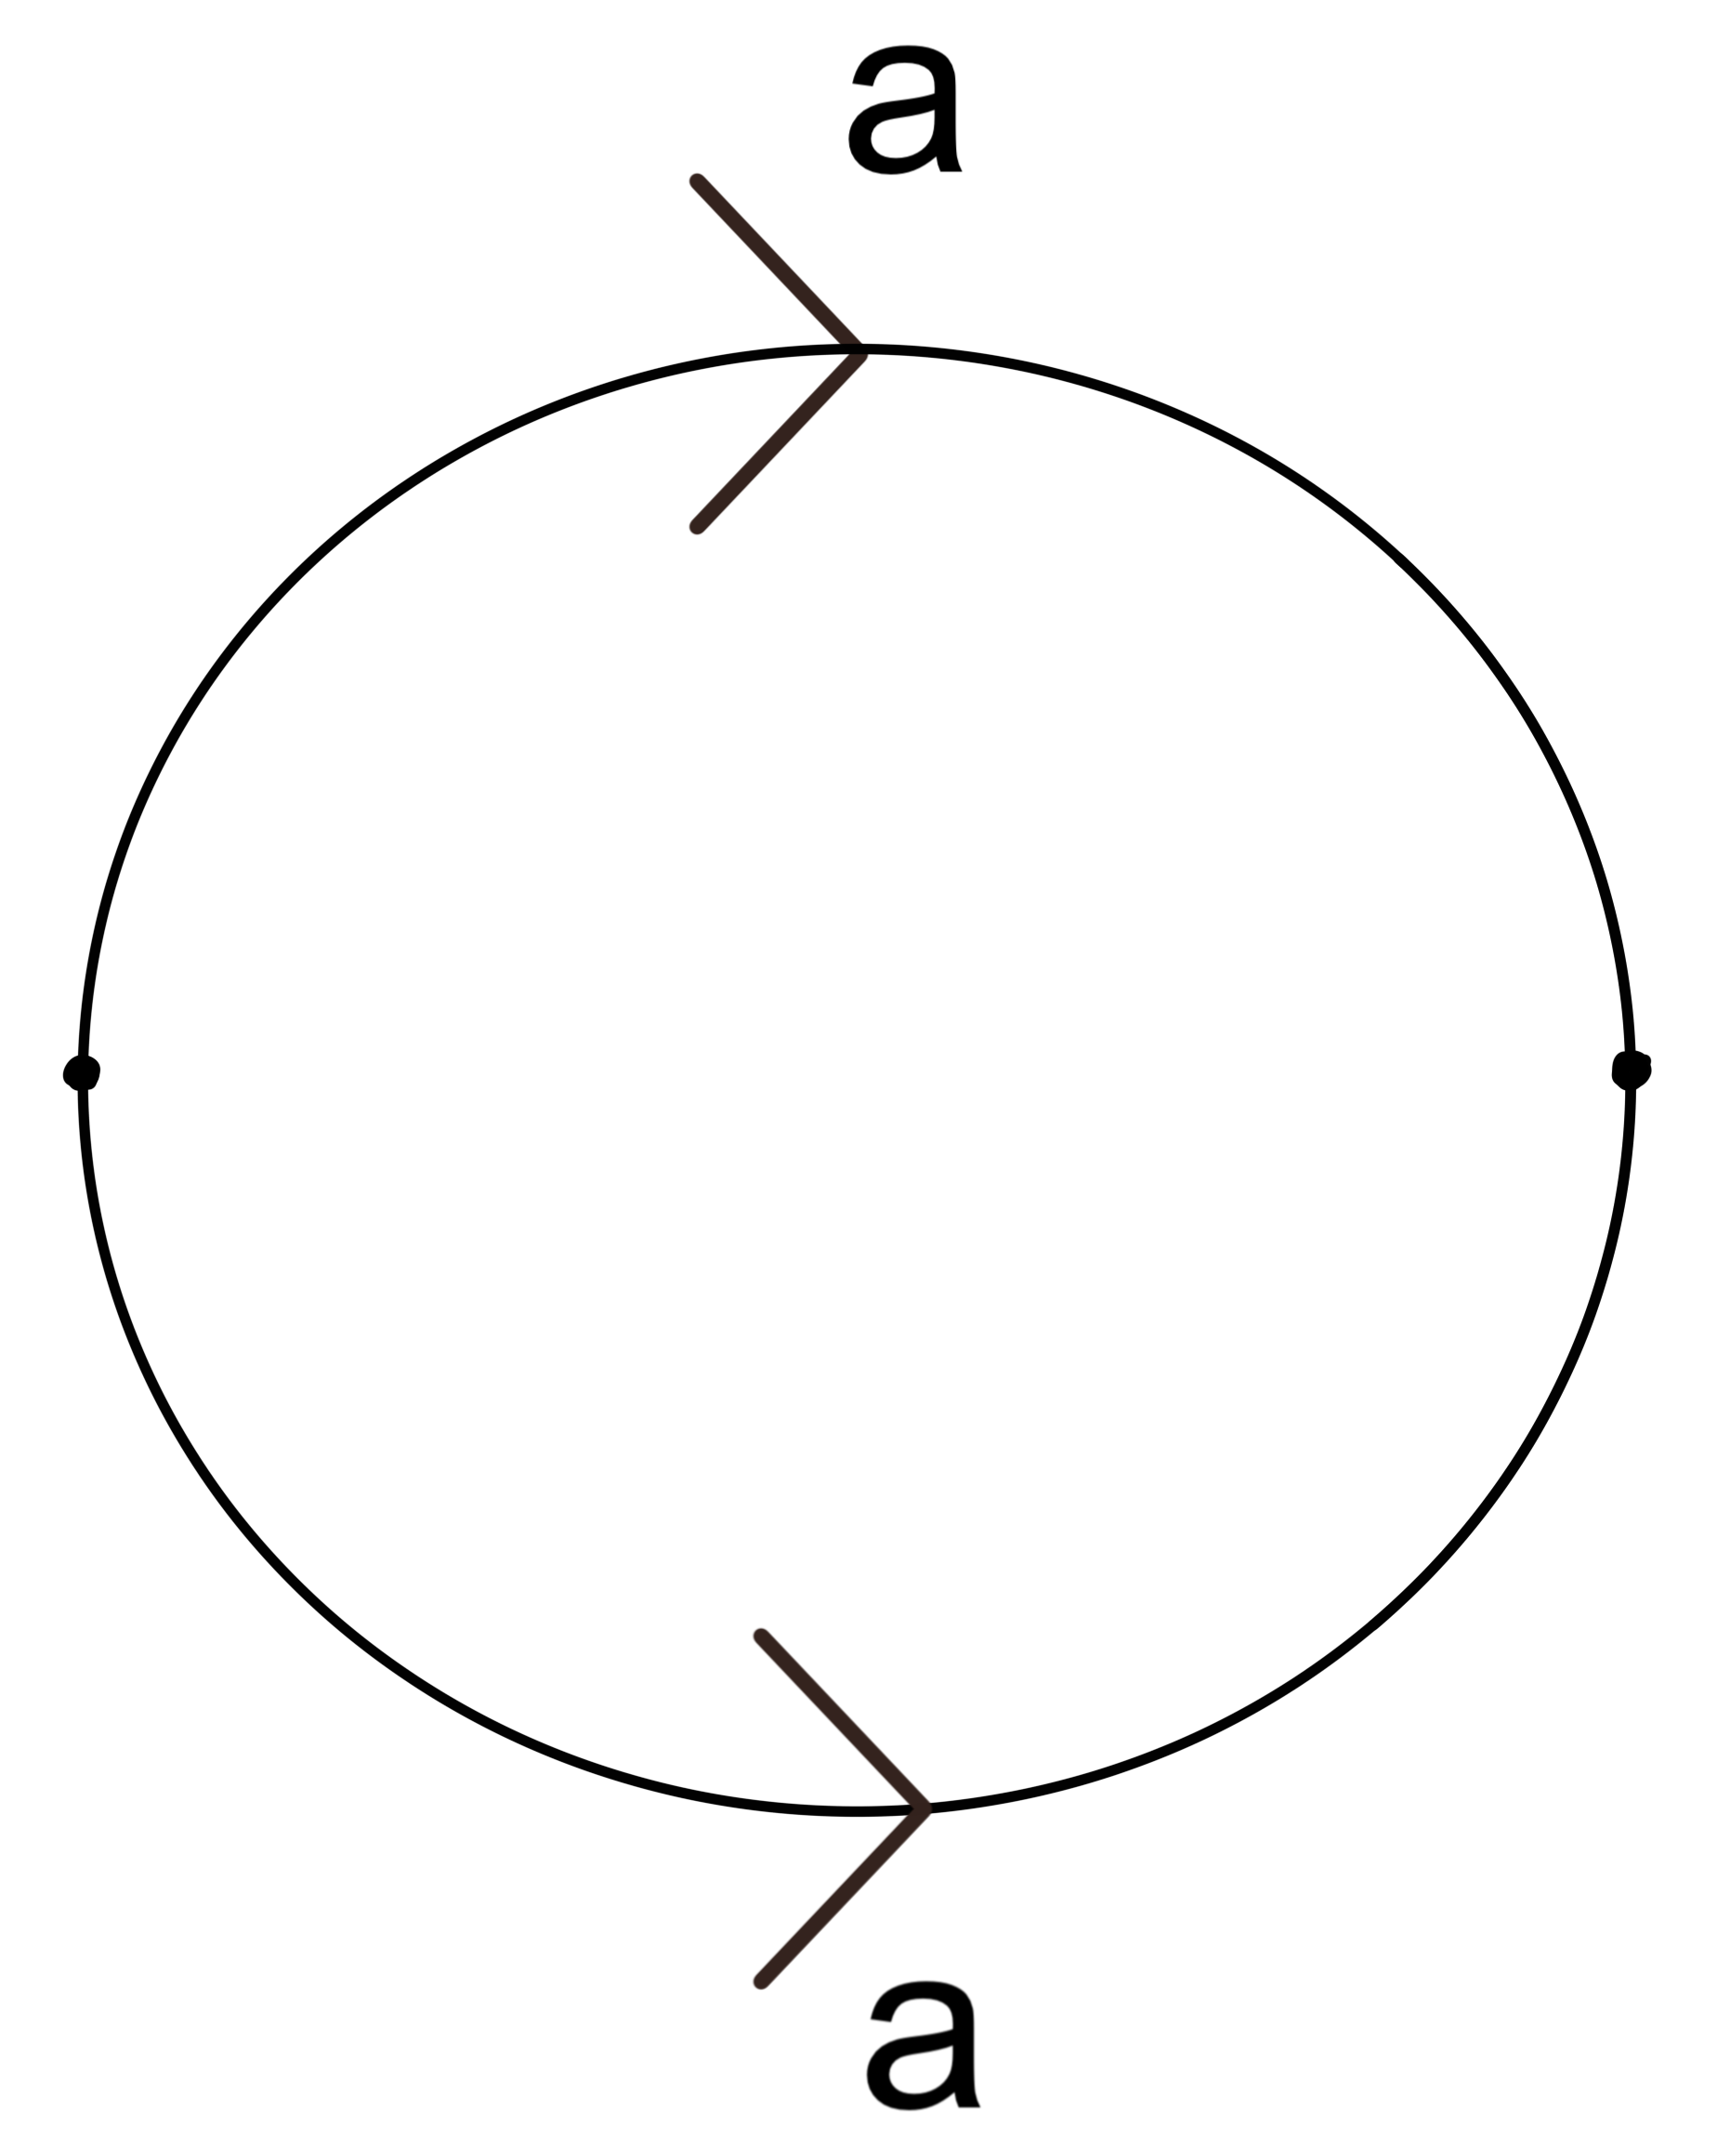
\includegraphics[width=0.15\linewidth]{imagenes/esfera_plana.png}
	\caption{Esfera como espacio cociente}
	\label{fig:esfera expresion canonica}
\end{figure} 


\subsection*{El toro}
Si se toma el cuadrado cerrado $ \overline{C} = \{ (x,y) \in R^2: -1\leq x\leq 1,\quad -1\leq y \leq 1  \} $ con la topología de subespacio, el \textit{toro}  se construye al identificar los puntos de  $ X $ según  \ref{toroid} y dotar al conjunto resultante de la topología cociente.
\begin{align}\label{toroid}
	(x,-1)\equiv(x,1) \quad x\in [-1,1]  \\
	(-1,y)\equiv(1,y) \quad y\in [-1,1] \nonumber
\end{align}
En la figura \ref{fig:toro expresion canonica} se representa gráficamente el toro. Las aristas con el mismo símbolo indican aquellas a identificar en el sentido fijado por las flechas.
\begin{figure}[h!]
	\centering
	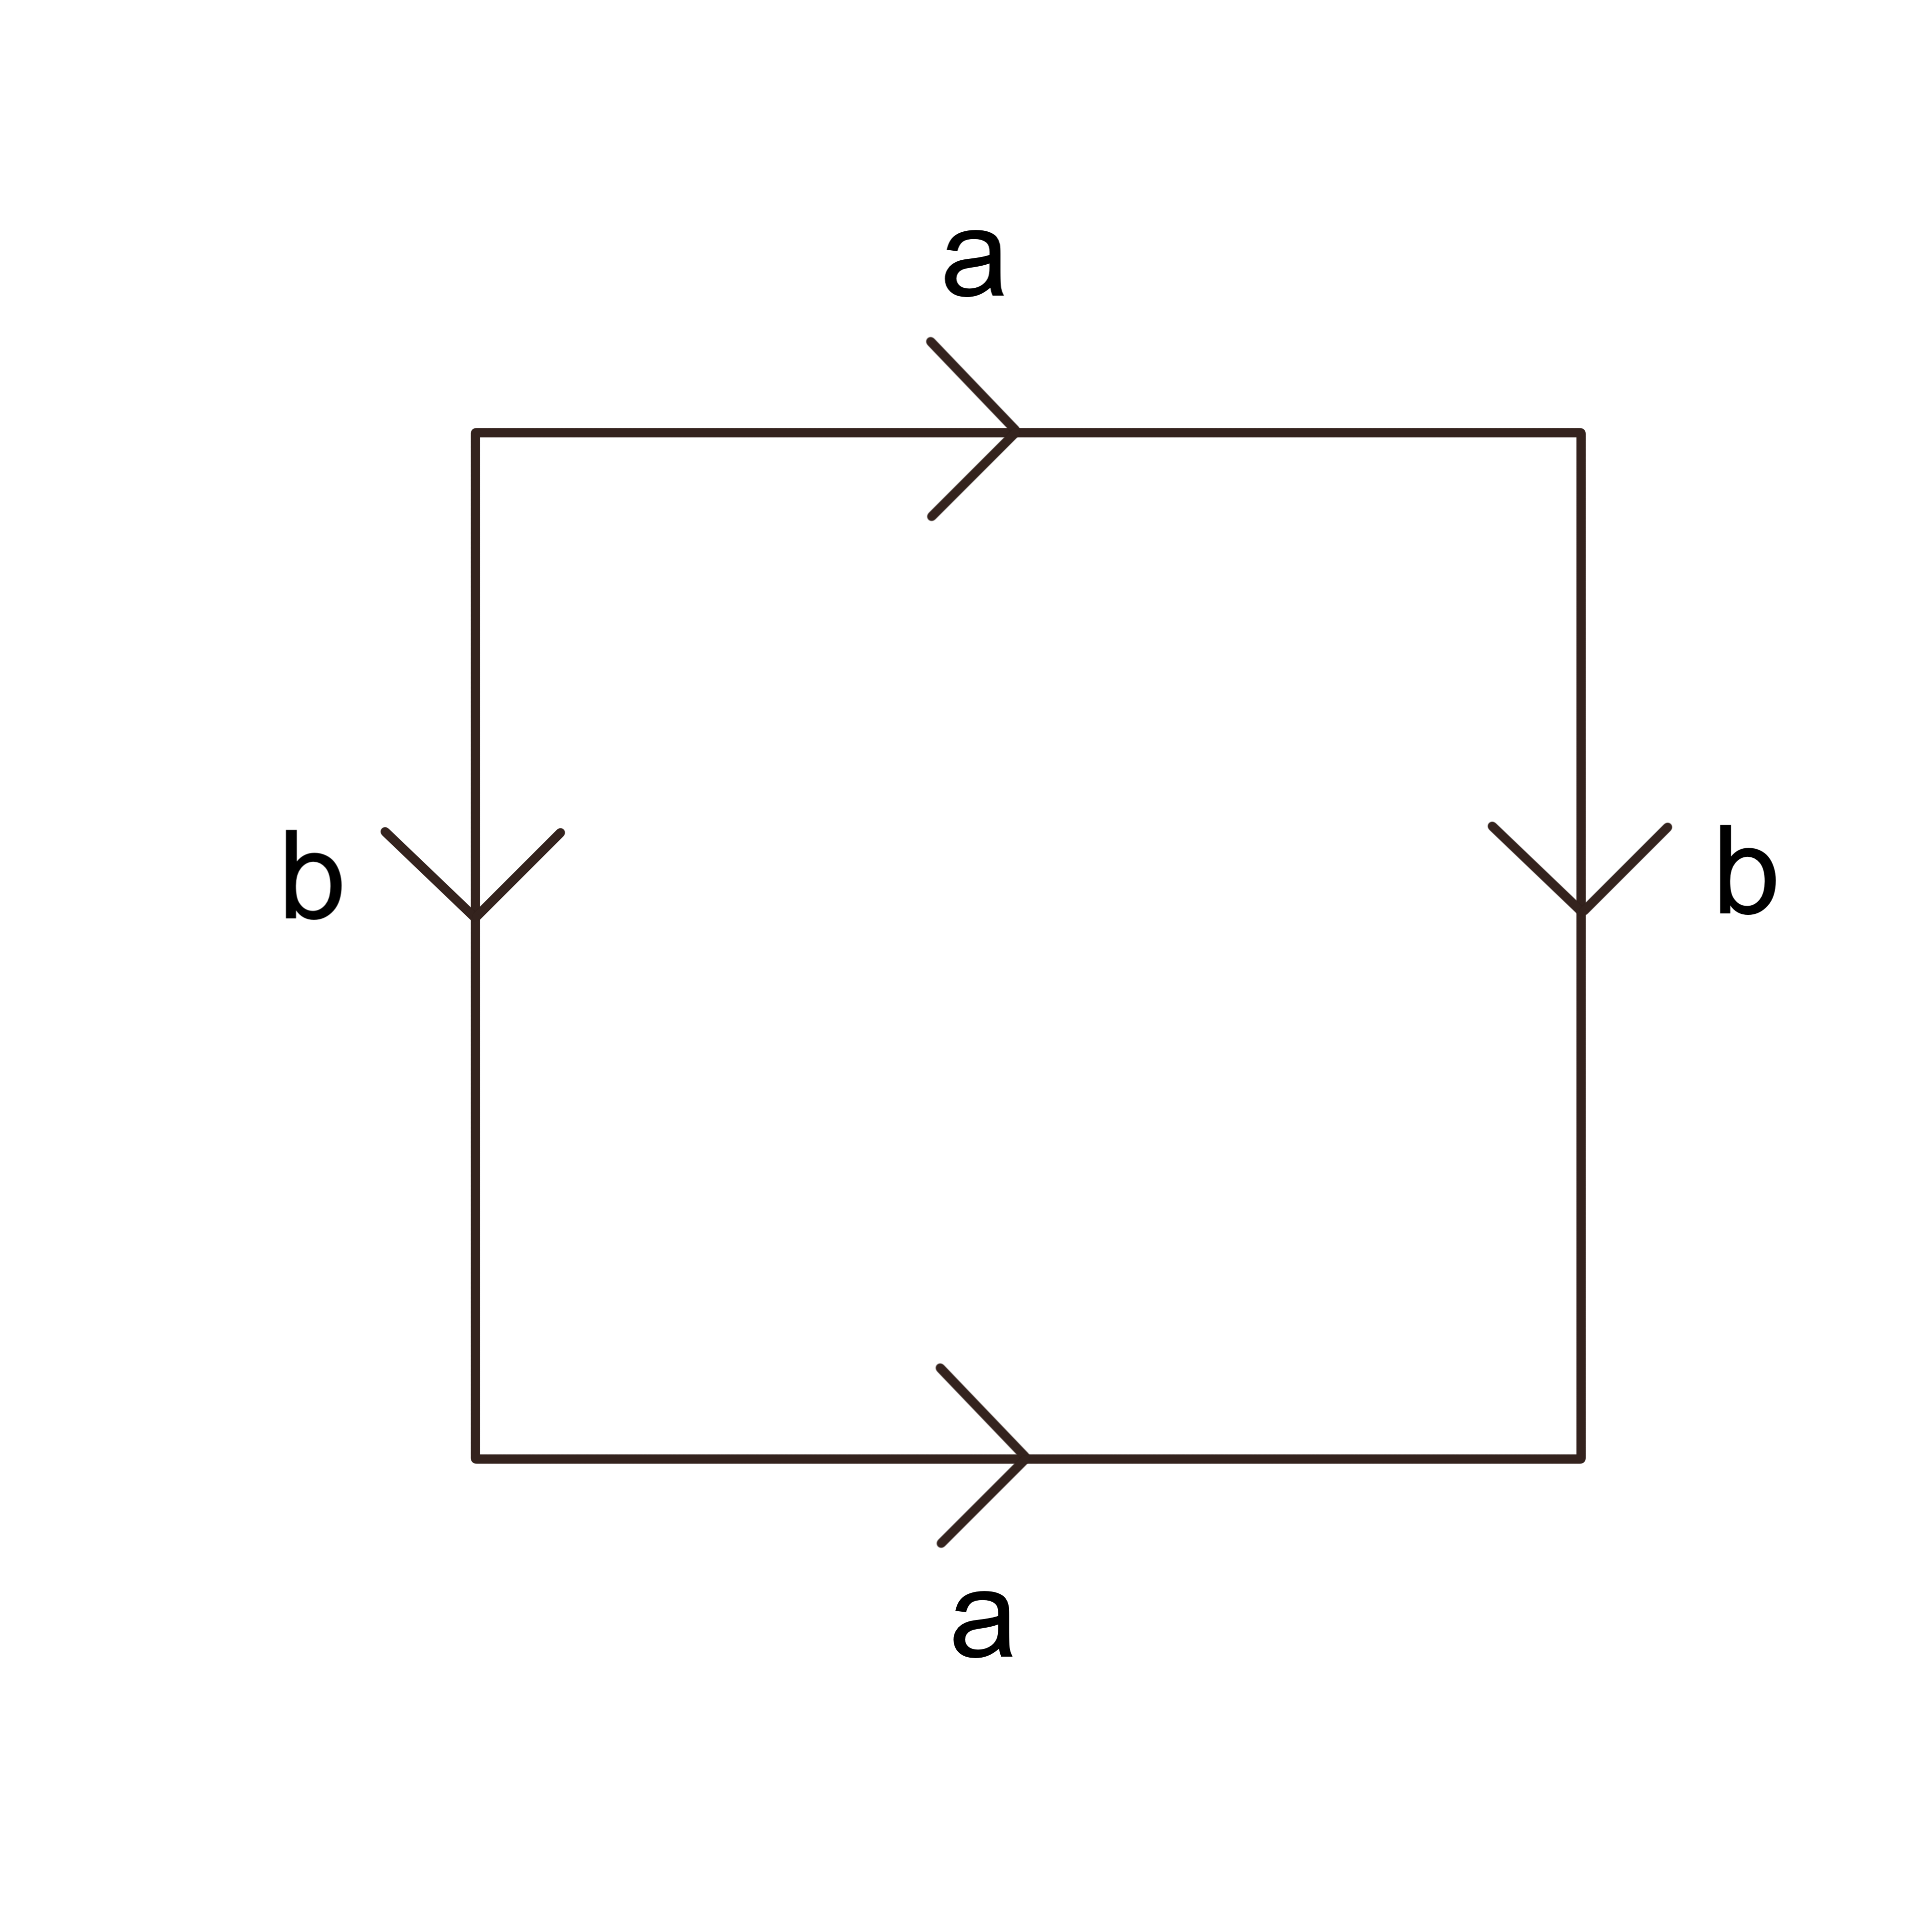
\includegraphics[width=0.2\linewidth]{imagenes/toroplano.png}
	\caption{Toro como espacio cociente}
	\label{fig:toro expresion canonica}
\end{figure} 

La definición de toro aquí expuesta es homeomorfa a la superficie de revolución en $\reales^3$ estudiada en el grado. Esta definición será conveniente más adelante en el teorema de clasificación de superficies compactas.

\subsection*{El plano proyectivo}
Por su parte, el \textit{plano proyectivo} corresponde al disco $ D = \{x\in\mathbb{R}^2: ||x||\leq1 \} $ en el cual se identifican los puntos antipodales de la frontera. Se ilustra esta identificación en la figura \ref{fig:planoproyectivo expresión canónica}.

\begin{figure}[h!]
	\centering
	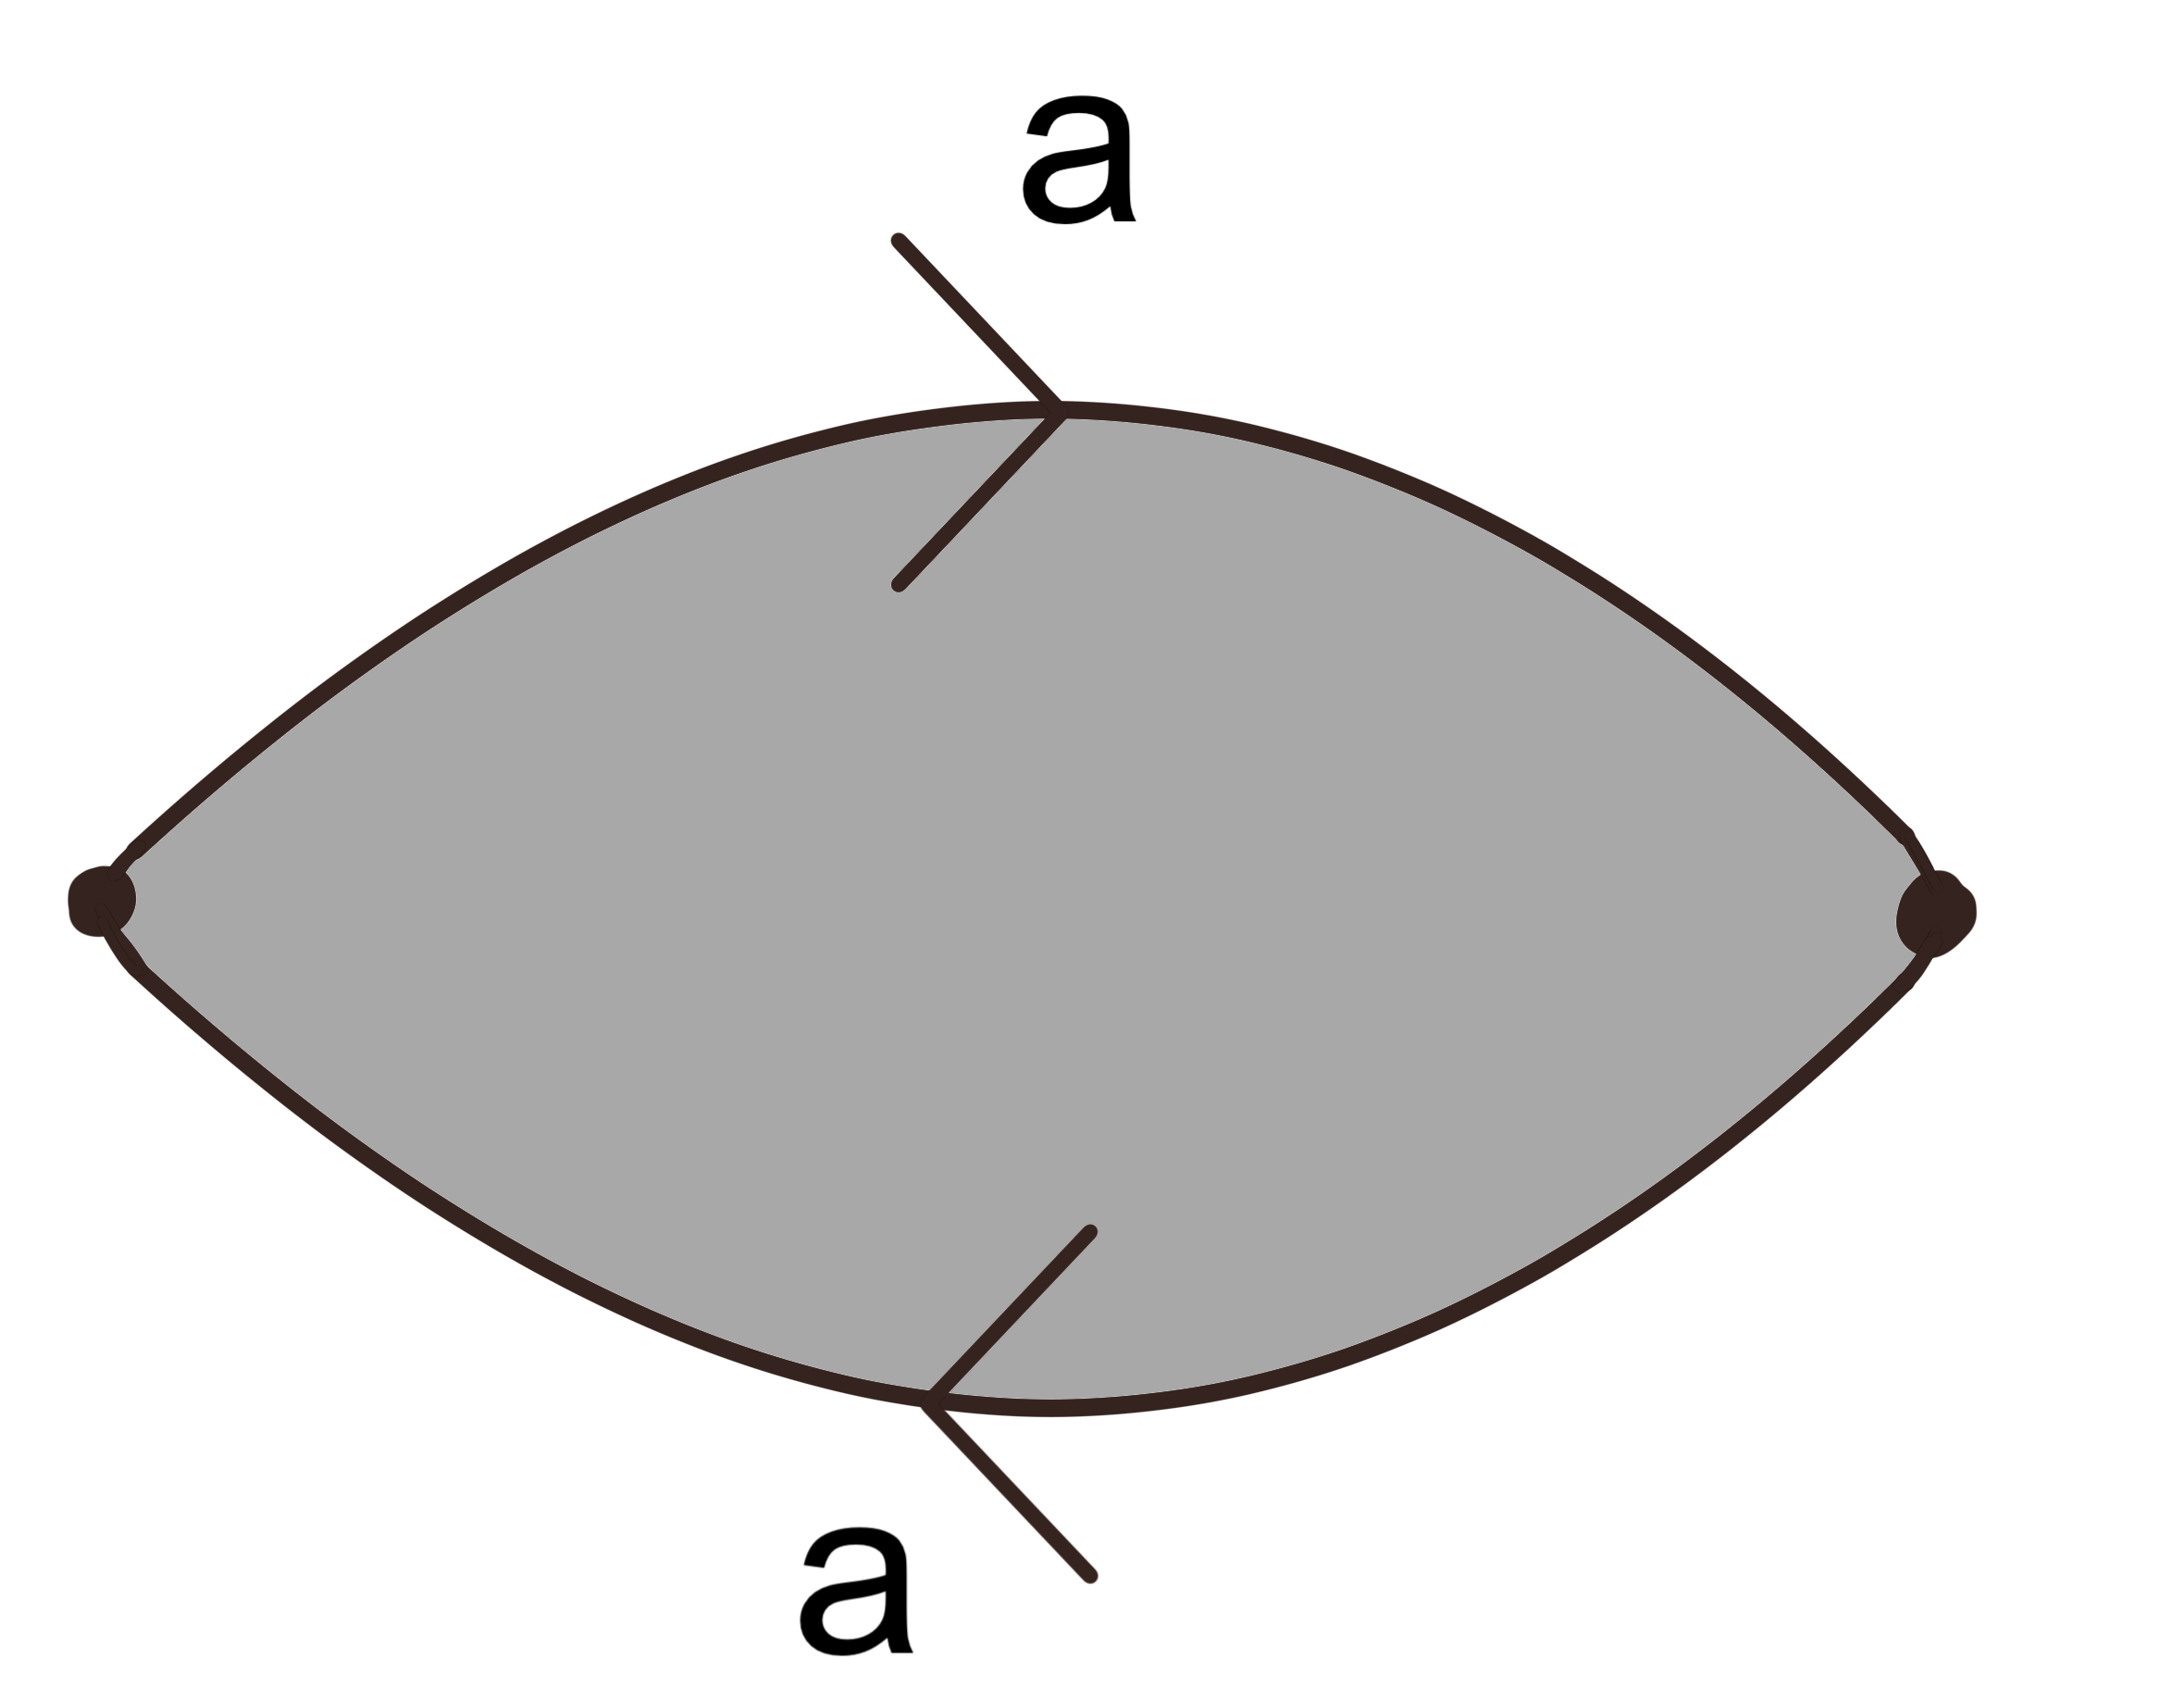
\includegraphics[width=0.3\linewidth]{imagenes/planop_plano.png}
	\caption{Plano proyectivo como espacio cociente}
	\label{fig:planoproyectivo expresión canónica}
\end{figure} 

De los tres ejemplos de superficies compactas dadas hasta ahora, este es el único de una superficie no orientable. 

Después de haber visto los ejemplos, es razonable cuestionarse si los espacios cocientes que tratamos son realmente conjuntos compactos. El siguiente lema nos demuestra que, en efecto, las superficies obtenidas son compactas.

\begin{lema}\label{lema:compacidadDePoligonos}
Sea $X$ un espacio topológico e $Y$  un espacio cociente que resulta de identificar puntos en $X$. Entonces:
\begin{align*}
	\text{$X$ compacto}\Rightarrow\text{$Y$ compacto}
\end{align*}
\end{lema}

\begin{proof}
Sea $f:X\longrightarrow Y$ la función cociente que asocia a cada punto su clase de equivalencia; $f$ es sobreyectiva y, por ser cociente, es continua.\\
Siendo $X$ compacto tenemos entonces que $f(X)=Y$ también lo es.
\end{proof}

En nuestros ejemplos todas las superficies vienen de identificar puntos en conjuntos compactos. Se sigue entonces del lema que las superficies son a su vez compactas.


\subsection{Expresión canónica}
\label{subsec:expcanonica}

Las figuras \ref{fig:esfera expresion canonica}, \ref{fig:toro expresion canonica} y \ref{fig:planoproyectivo expresión canónica}, de cada ejemplo respectivamente, sugieren una forma visual de definir superficies compactas: formamos un polígono con un número par de lados e identificamos sus aristas por parejas. 

Más aún, se puede definir una notación con la que referirnos a estos polígonos: \\
Partiendo de cualquier vértice recorremos la figura en el sentido de las agujas del reloj, se anotan los símbolos según se recorre la respectiva arista y se agrega el exponente 1 o -1, según si la flecha va en el mismo sentido del recorrido o en sentido contrario.

Con esta notación: nos referimos  a la esfera (figura \ref{fig:esfera expresion canonica}) como $ aa^{-1} $; al toro (figura \ref{fig:toro expresion canonica})  como $ aba^{-1}b^{-1} $; y al plano proyectivo (figura \ref{fig:planoproyectivo expresión canónica}) como $ aa $. Llamaremos \textit{expresión canónica} a estas formas de referirnos a la esfera, al toro y al plano proyectivo, respectivamente.

La notación sugerida facilita enormemente la definición de nuevas superficies. Utilicemos esta herramienta para introducir un último ejemplo de superficie compacta:


\subsection*{Botella de Klein}
La \textit{botella de Klein} es la superficie que corresponde con la expresión $ aba^{-1}b $.
\begin{figure}[h!]
	\centering
	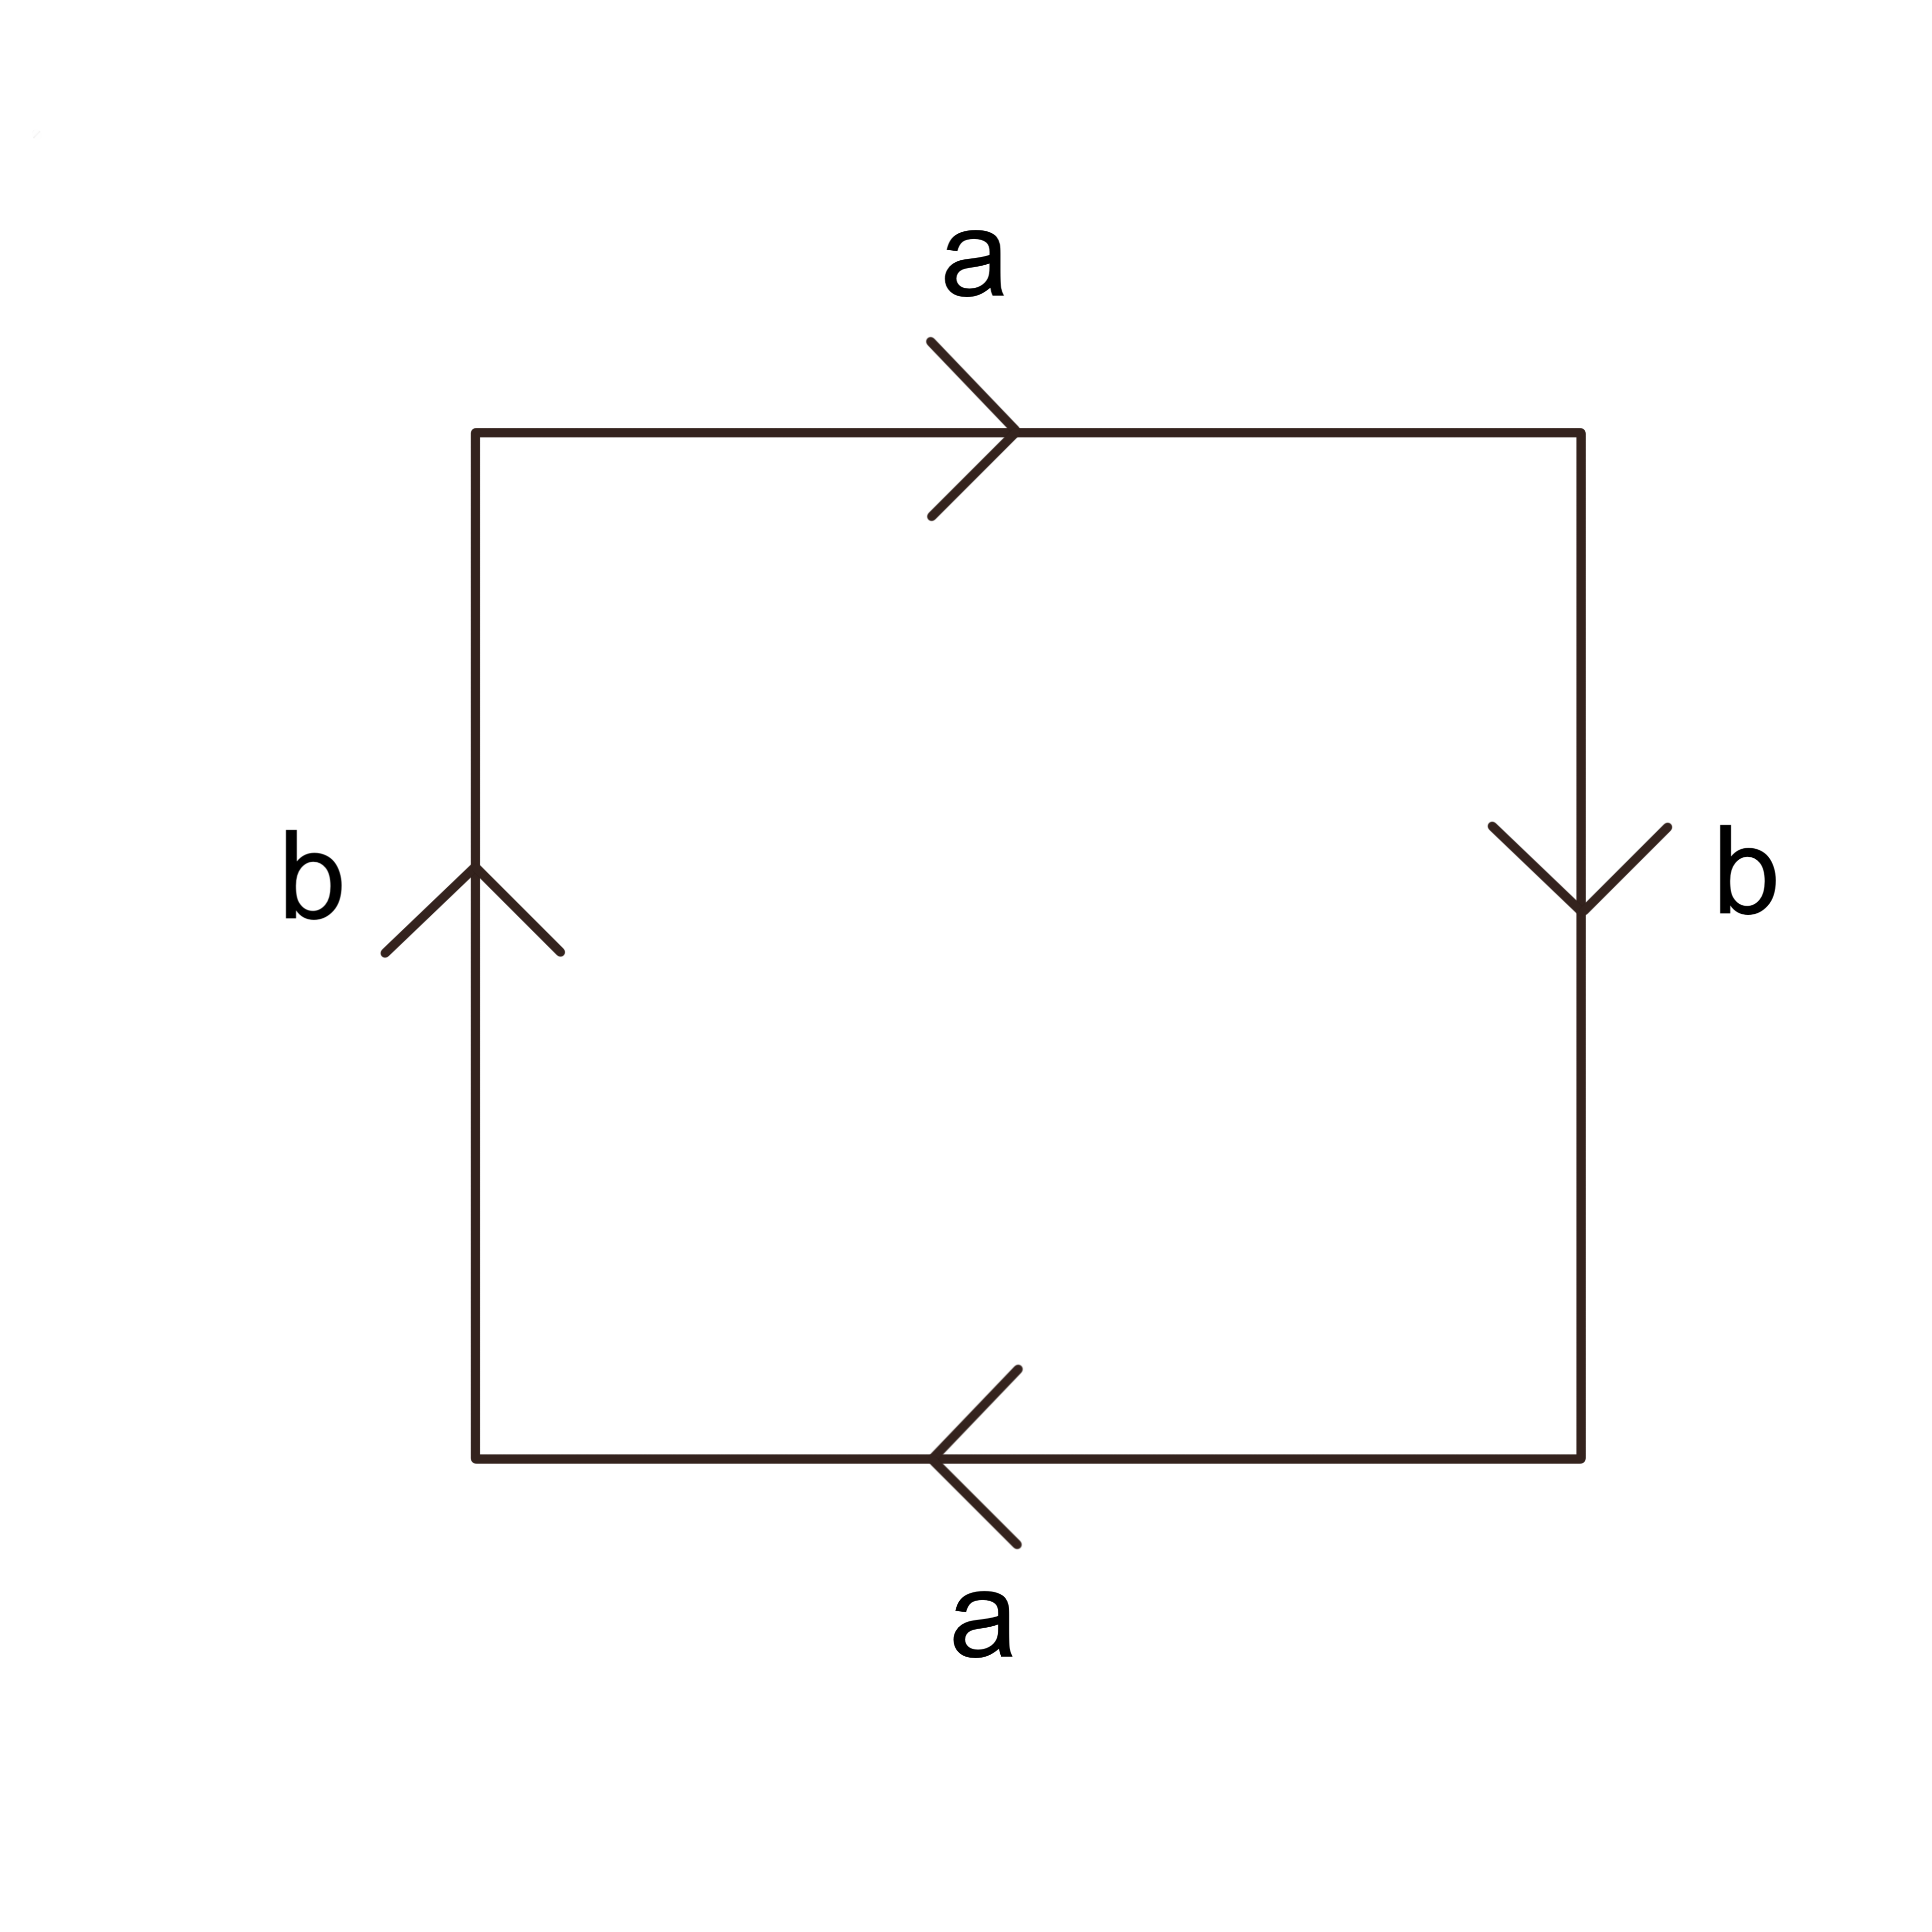
\includegraphics[width=0.2\linewidth]{imagenes/klein.png}
	\caption{Botella de Klein}
	\label{fig:botelladeklein expresion canónica}
\end{figure} 

La botella de Klein compone un ejemplo de superficie no orientable que, además, no es representable en $\reales^3$ como una superficie regular.

\section{Suma conexa}
\label{sec:sumaconexa}
La suma conexa es un operador entre superficies. La idea será ir `sumando' superficies compactas para generar nuevas. De hecho, si se me permite el \textit{spoiler}, utilizaremos este operador en toros y planos proyectivos para construir superficies homeomorfas a cualquier otra superficie compacta.\\
Procedamos a definir matemáticamente el operador:

\begin{defin}\label{defin:sumaconexa}
Dadas dos superfices $S_1$ y $S_2$, se define la \textit{suma conexa} de ambas ($S_1\#S_2$) como la superficie generada al recortar un disco de cada superficie y pegarlas a través del borde de los discos retirados. Más formalmente:
\begin{enumerate}
\item  Para cada $S_i$, tomamos un subconjunto $D_i\subset S_i$ homeomorfo al disco cerrado $E^2=\{x\in\mathbb{R}^2: ||x||\leq 1\}$. Llamamos $S'_i$ al complementario del interior de $D_i$.

\item Tomamos un homeomorfismo $\psi:D_1\longrightarrow D_2$

\item Definimos entonces $S_1\#S_2$ como $S'_1\cup S'_2$ dotado de la topología cociente que resulta de la identificación:
\[ x \equiv  \psi(x), \quad \forall x \in D_1 \] 
\end{enumerate}
Se puede comprobar que el resultado de la suma conexa es otra superficie y que no depende ni de los discos elegidos, ni del homeomorfismo $\psi$.
\end{defin}


\subsection*{Ejemplos}
Utilizando la notación introducida hasta el momento presentamos algunos ejemplos de sumas conexas:

\noindent \textbf{Suma conexa de toros}
\\
Sean $ T_1 $ y $ T_2 $ dos toros disjuntos, estudiemos $ S=T_1\, \# \, T_2 $. Nos ayudamos de la figura \ref{fig:suma conexa de toros planos} para ilustrar el proceso:\\
Primero, retiramos de cada toro el disco con frontera $c_i$, como vemos en la primera imagen. Nótese que podemos expresarlo como la segunda imagen porque todos los vértices del polígono están identificados. Finalmente, identificamos los bordes $ c_1 $ y $ c_2 $, obteniendo el octágono que representa  $ S $, donde, de nuevo, todos los vértices representan el mismo punto.

\begin{figure}[h!]
	\centering
	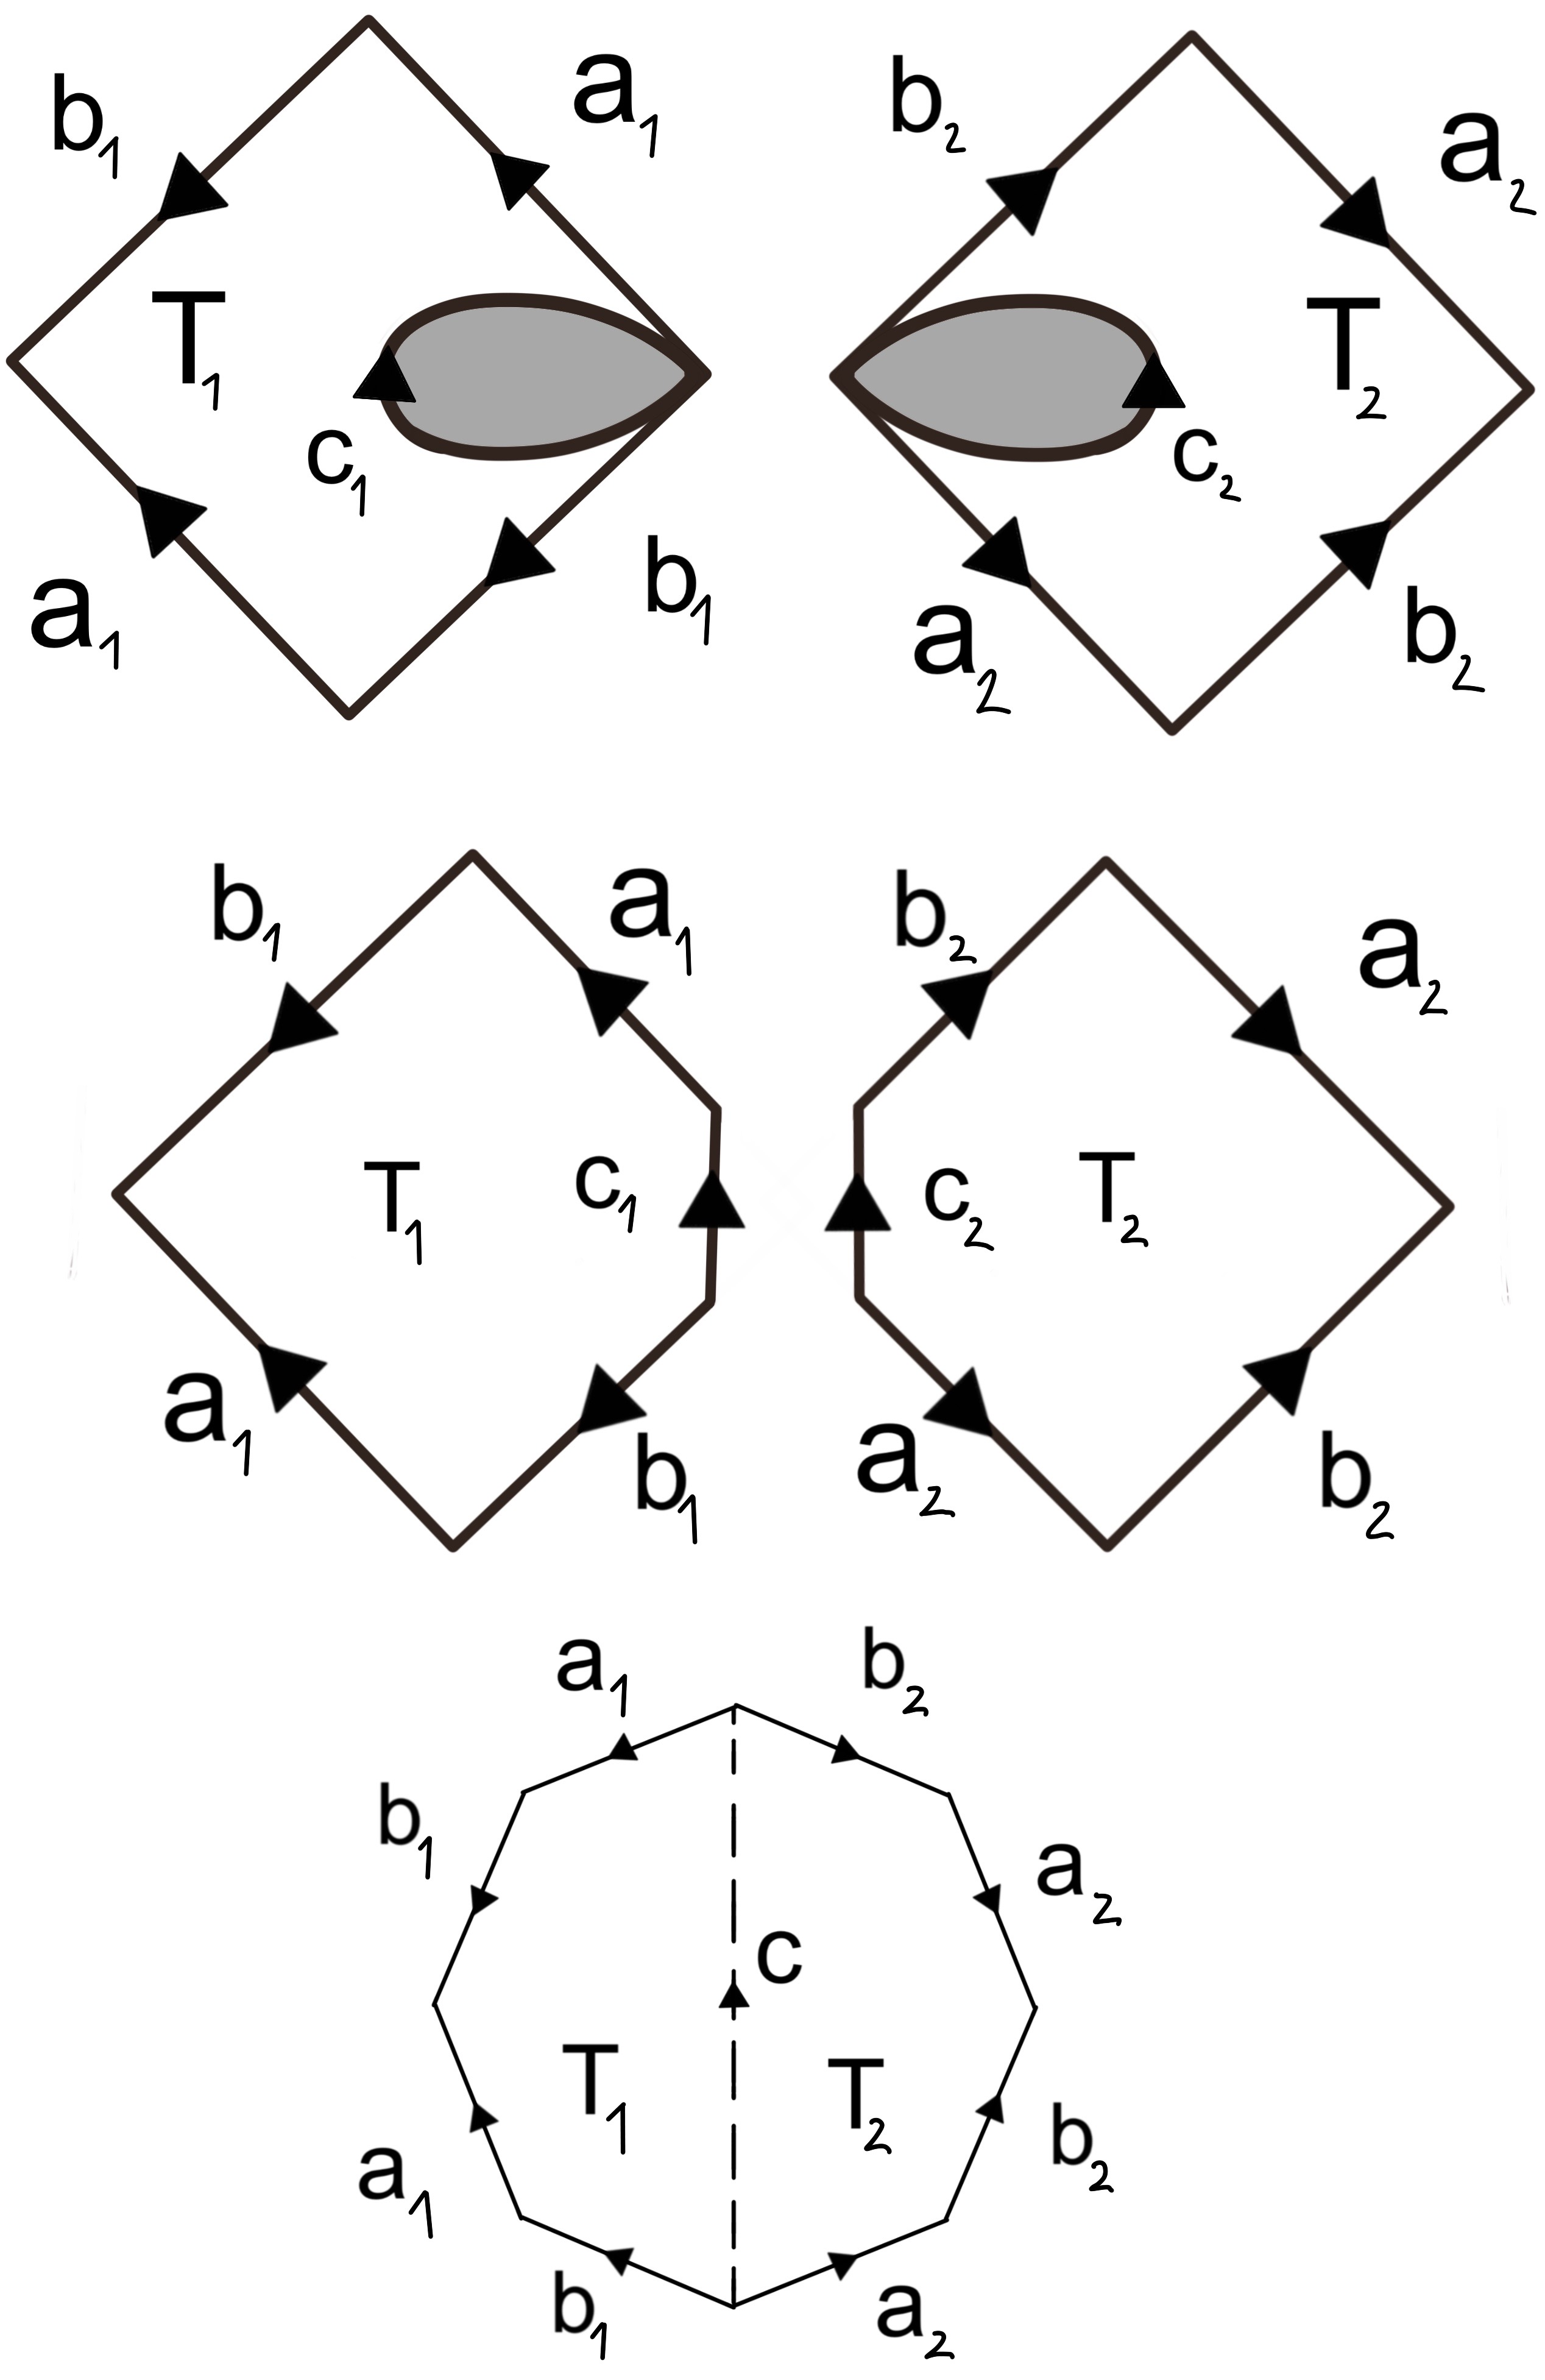
\includegraphics[width=0.4\linewidth]{imagenes/sumaconexa_toros.png}
	\caption{Suma conexa de dos toros}
	\label{fig:suma conexa de toros planos}
\end{figure} 

Utilizando la notación para expresiones canónicas, de la figura \ref{fig:suma conexa de toros planos} se deduce que  $ S $ se puede expresar como $ a_1 b_1 a_1^{-1}b_1^{-1}a_2 b_2 a_2^{-1} b_2^{-1}  $. 

\begin{figure}[h!]
	\centering
	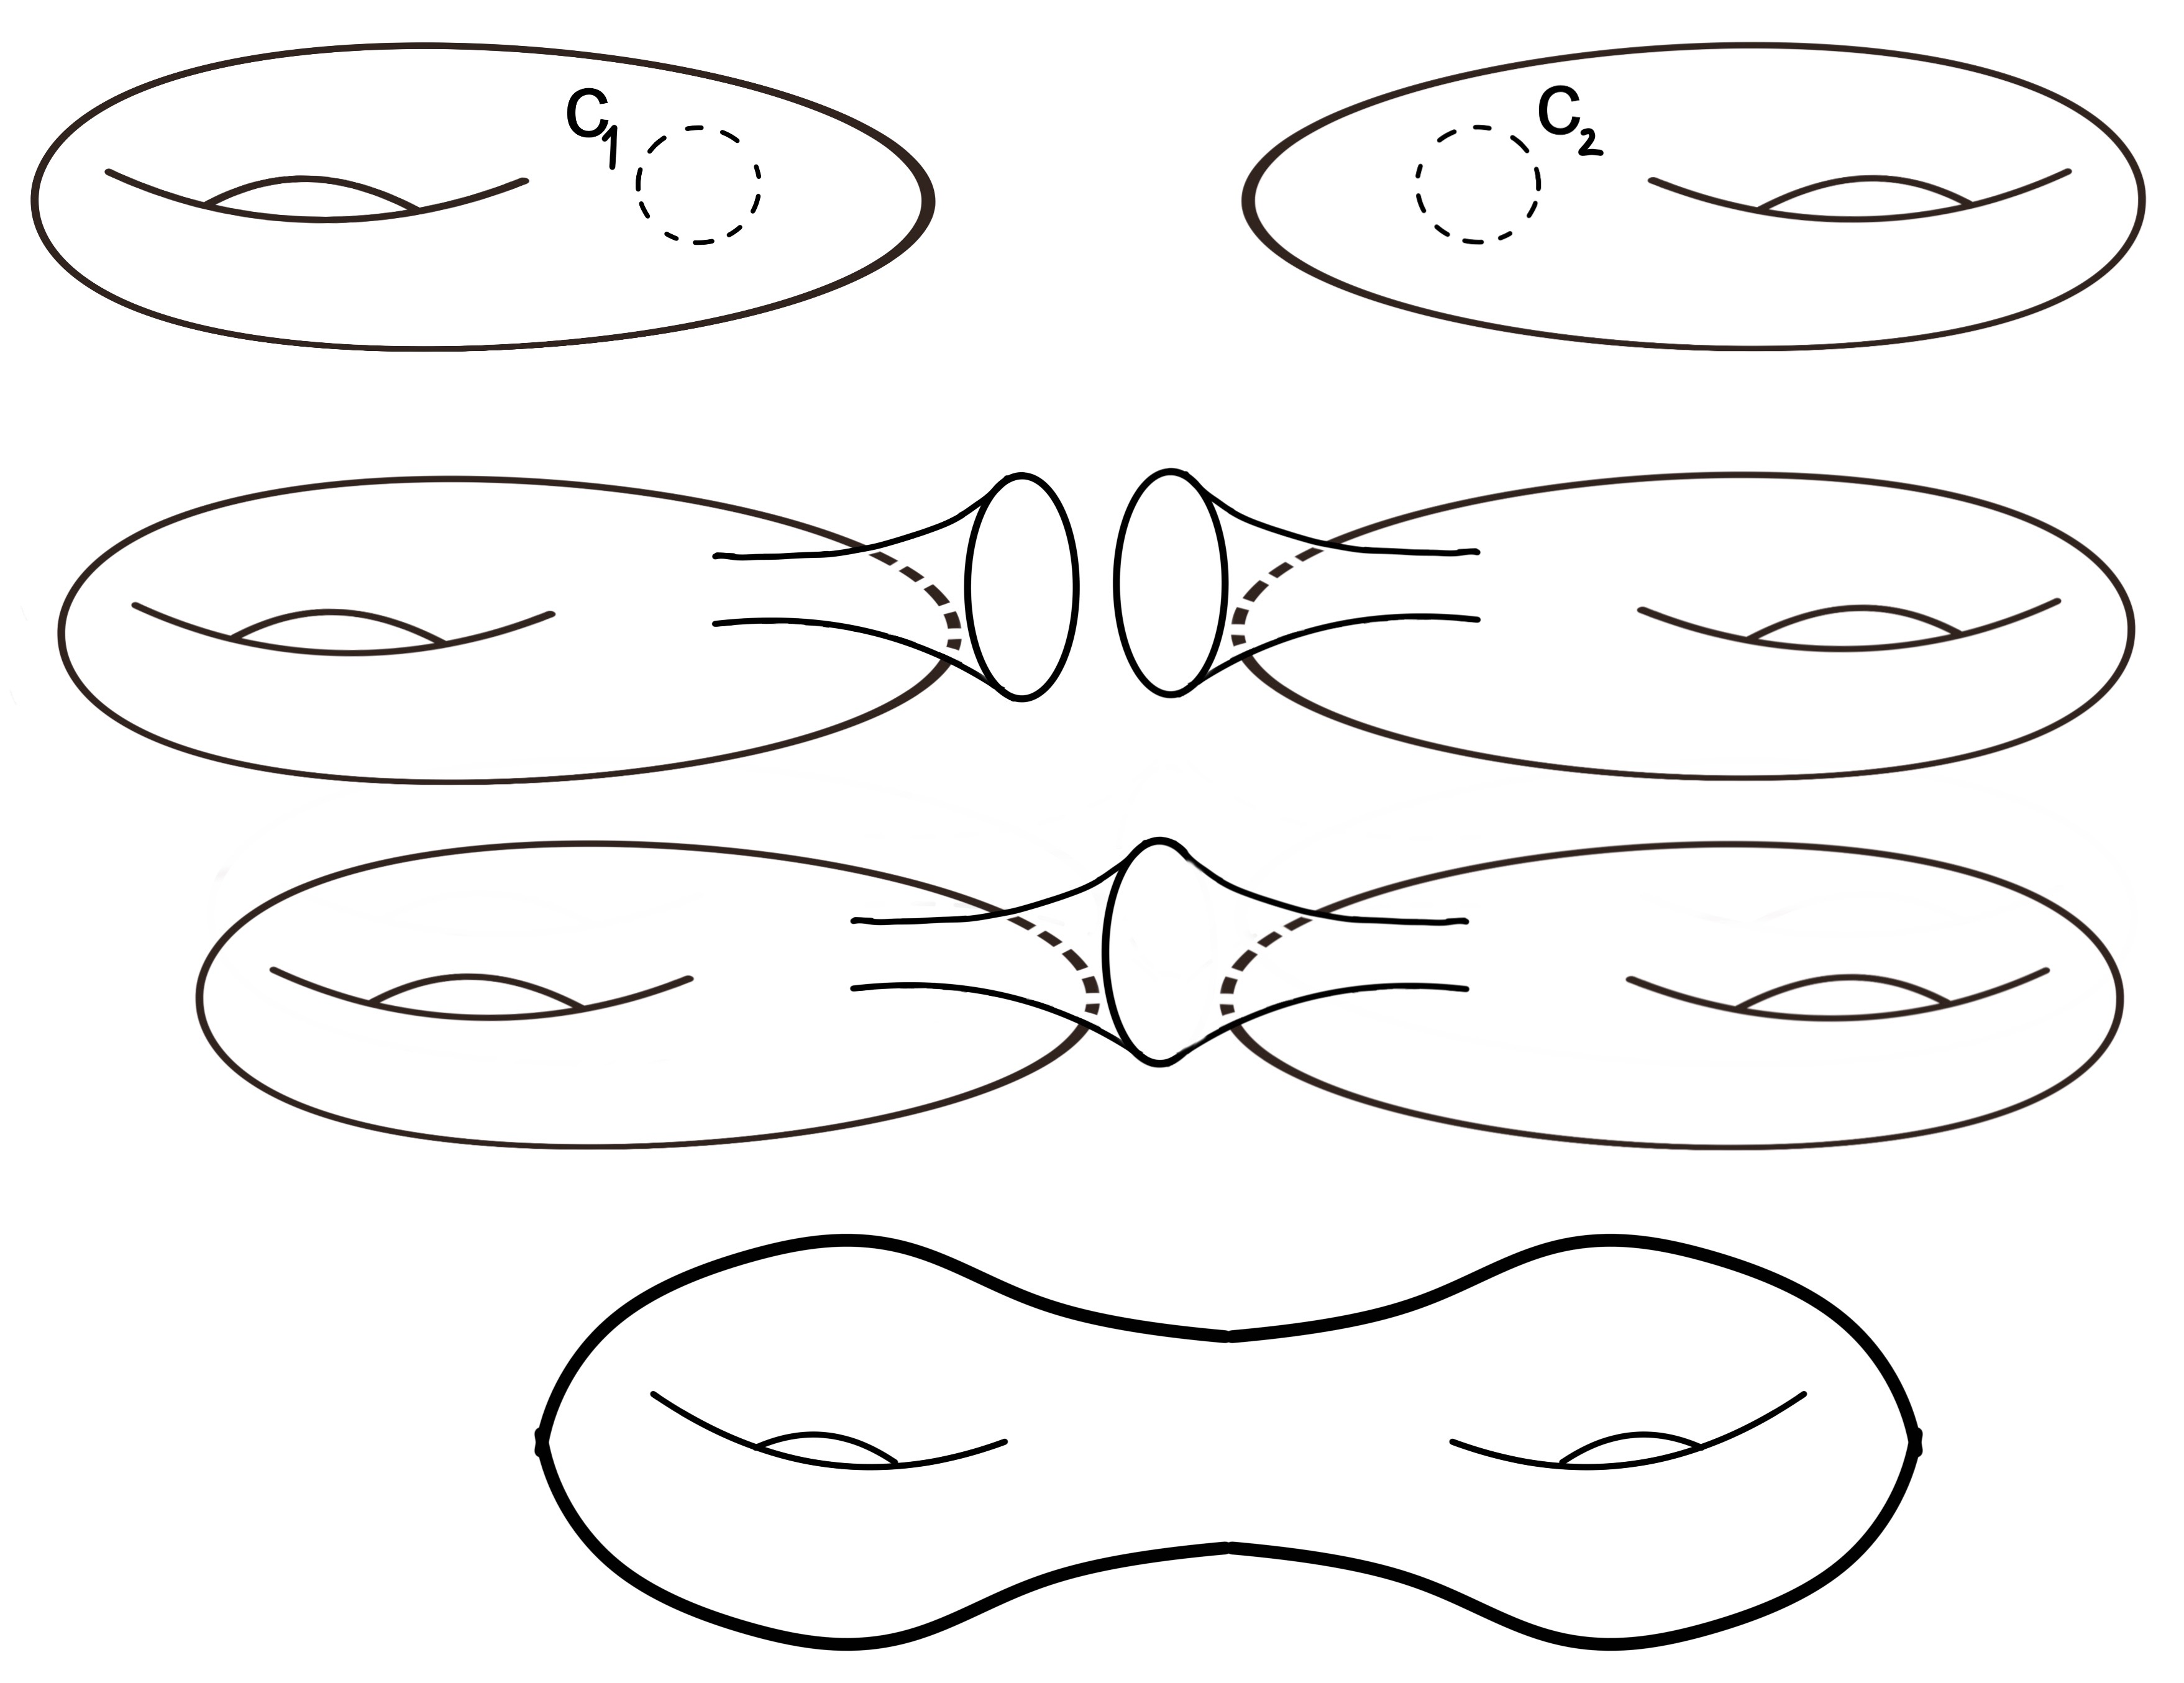
\includegraphics[width=0.4\linewidth]{imagenes/sumaconexa_toros_R3.png}
	\caption{Suma conexa de dos toros como subvariedades de $ \mathbb{R}^3 $}
	\label{fig:suma conexa de toros en R3}
\end{figure} 

\noindent \textbf{Suma conexa de planos proyectivos}
\\
Podemos seguir un mecanismo parecido al anterior para realizar la suma conexa de dos planos proyectivos. En la figura \ref{fig:suma conexa de planos p} ilustramos la misma construcción para dos planos proyectivos. La expresión canónica de la superficie resultante es $ a_1a_1a_2a_2 $.

\begin{figure}[h!]
	\centering
	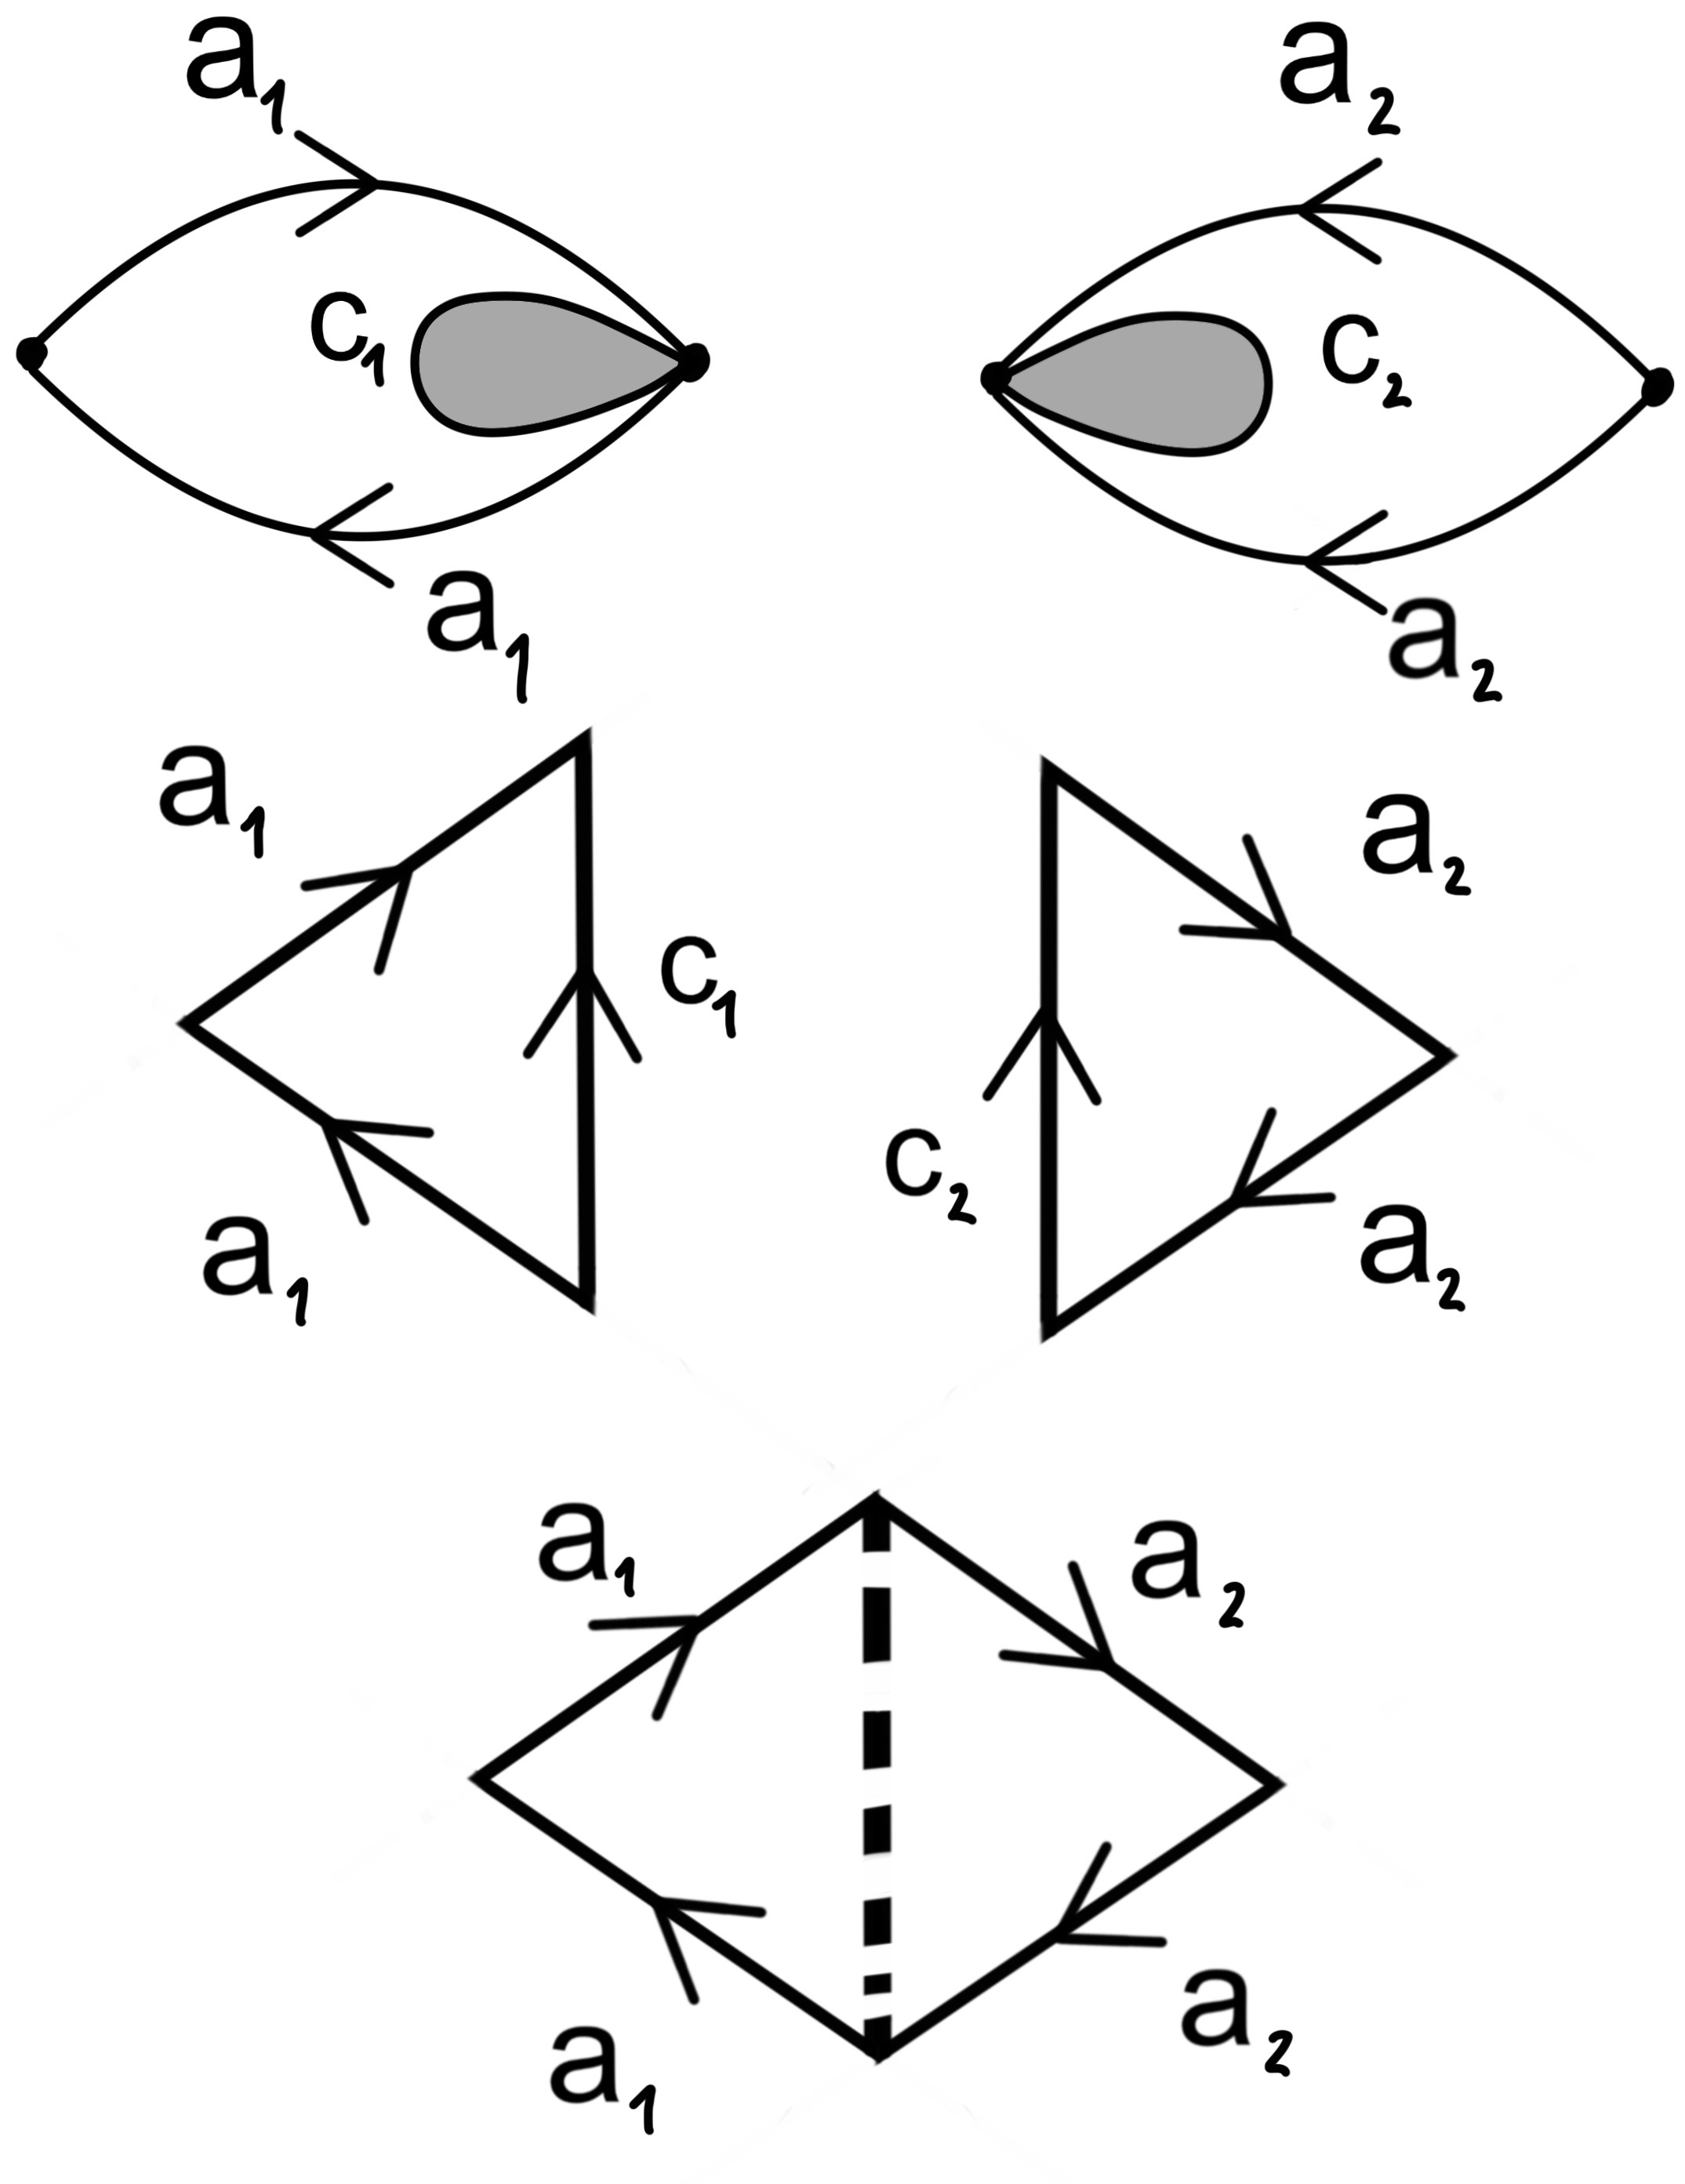
\includegraphics[width=0.3\linewidth]{imagenes/sumaconexa_planosp.png}
	\caption{Suma conexa de dos planos proyectivos}
	\label{fig:suma conexa de planos p}
\end{figure} 

\noindent \textbf{Suma conexa de esferas}
\\
En la figura \ref{fig:suma conexa de esferas} ilustramos la suma conexa de dos esferas, que es otra esfera. En general, se puede comprobar que la esfera actúa como elemento neutro de la suma conexa.

\begin{figure}[h!]
	\centering
	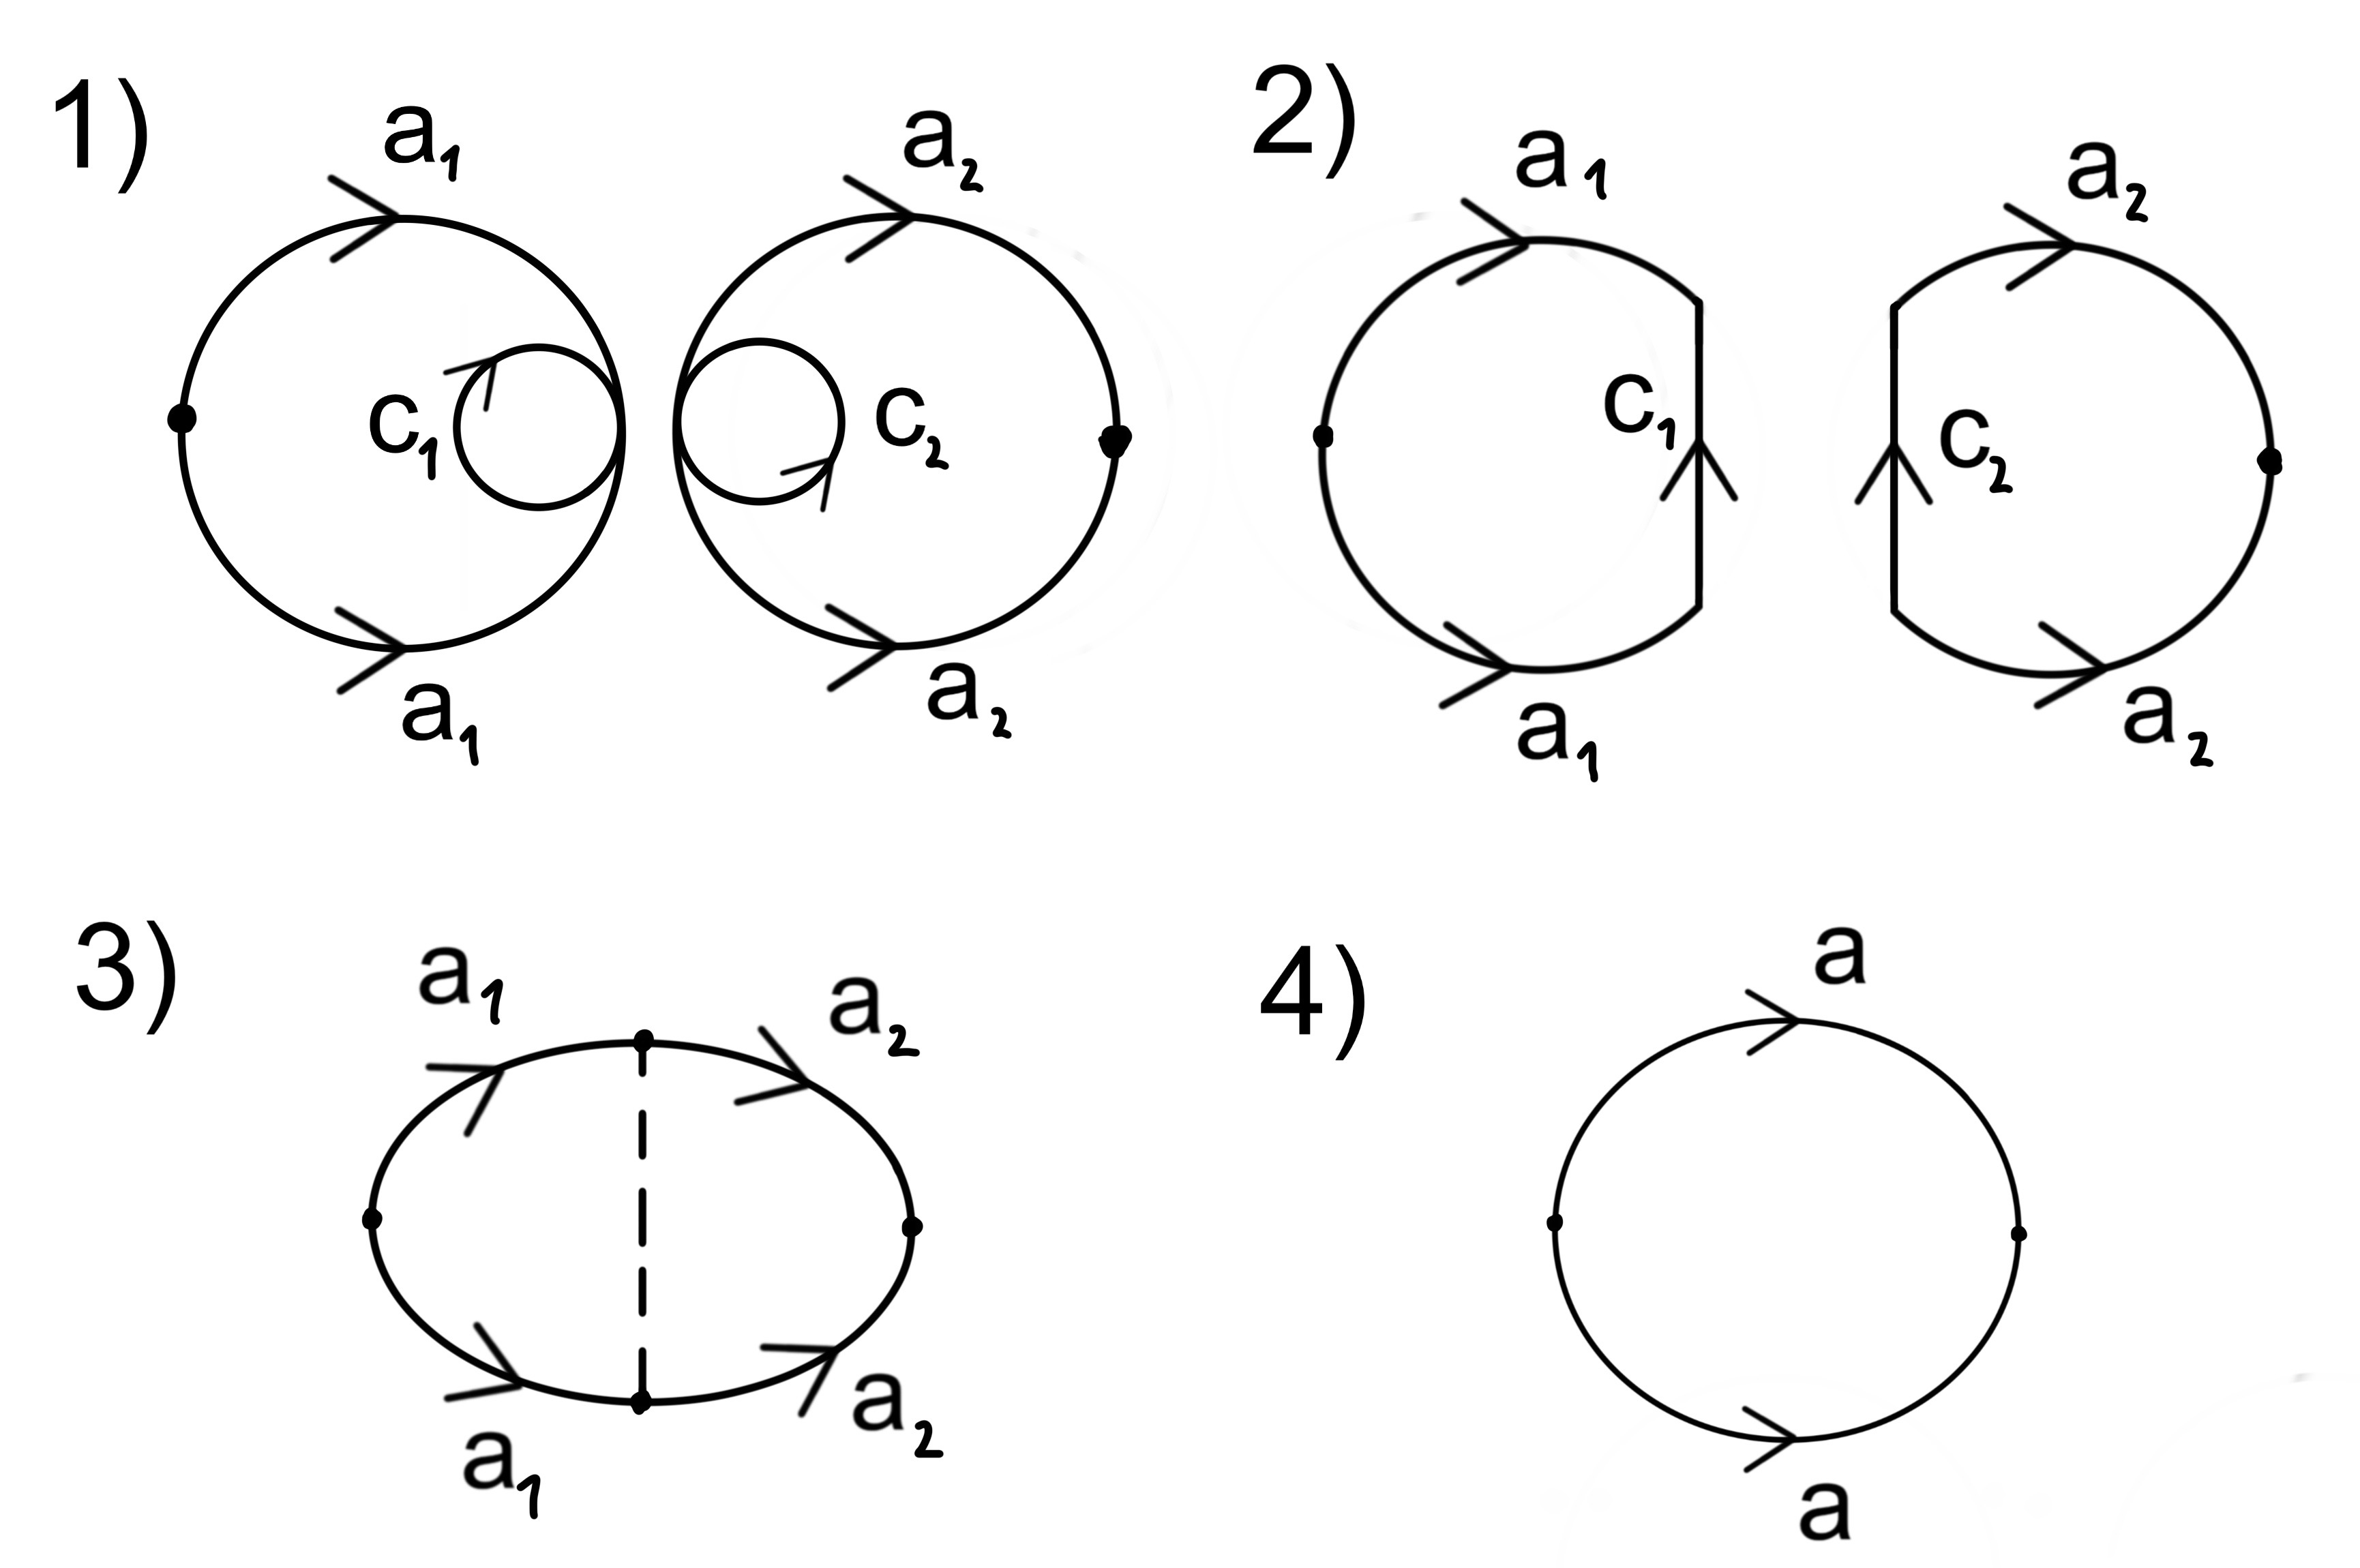
\includegraphics[width=0.5\linewidth]{imagenes/sumaconexa_esferas.png}
	\caption{Suma conexa de dos esferas}
	\label{fig:suma conexa de esferas}
\end{figure} 

Otra propiedad interesante de la suma conexa es que conserva la compacidad, i.e, si $S=S_1 \, \# \, S_2$, entonces $S$ será compacta si lo son $S_1$ y $S_2$. En los ejemplos de la suma de toros, planos proyectivos y esferas, basta con usar el lema \ref{lema:compacidadDePoligonos} para demostrarlo.

\subsection{Expresiónes canónicas de sumas conexas}
\label{subsec:expresionescanonicassumasconexas}
Los ejemplos mencionados en la sección anterior proporcionan un método para describir sumas conexas arbitrarias de esferas, toros y planos proyectivos. Basta repetir los mismos procedimientos para comprobar que:

\begin{list}{-}{}
\item La suma conexa de $ n $ esferas es igual a una esfera:
\begin{align}\label{formacanonica:esfera}
	aa^{-1} 
\end{align}

	\item La suma conexa de $ n $ toros se puede escribir como:
\begin{align}\label{formacanonica:ntoros}
	a_1b_1a_1^{-1}b_1^{-1}a_2b_2a_2^{-1}b_2^{-1}...a_nb_na_n^{-1}b_n^{-1}
\end{align}

	\item La suma conexa de $ n $ planos proyectivos se puede describir como: 
\begin{align}\label{formacanonica:nplanosp}
a_1a_1a_2a_2...a_na_n
\end{align}
\end{list}
A las expresiones \ref{formacanonica:esfera},\ref{formacanonica:ntoros} y \ref{formacanonica:nplanosp} las llamaremos \textit{expresiones canónicas} de sus respectivas sumas conexas.
 
Antes de dar el asunto por concluido, veamos un último ejemplo de suma conexa:

\begin{lema}\label{lema:SumaDosPlanospEsKlein}
La suma conexa de dos planos proyectivos es homeomorfa a una botella de Klein

\begin{proof}
En la demostración trataremos al plano proyectivo como el disco unidad identificando los puntos diametralmente opuestos.\\
Seleccionamos del plano proyectivo el subconjunto $D = \left\{(x,y): ||y||\geq\frac{1}{2}, ||x||\leq\sqrt{1-y^2} \right\}$  homeomorfo al disco cerrado. Retiramos $ D $ como se muestra en la figura \ref{fig:planop sin D}, los segmentos discontinuos representan la frontera del disco por la cual se ha de realizar la suma conexa.

\begin{figure}[h!]
	\centering
	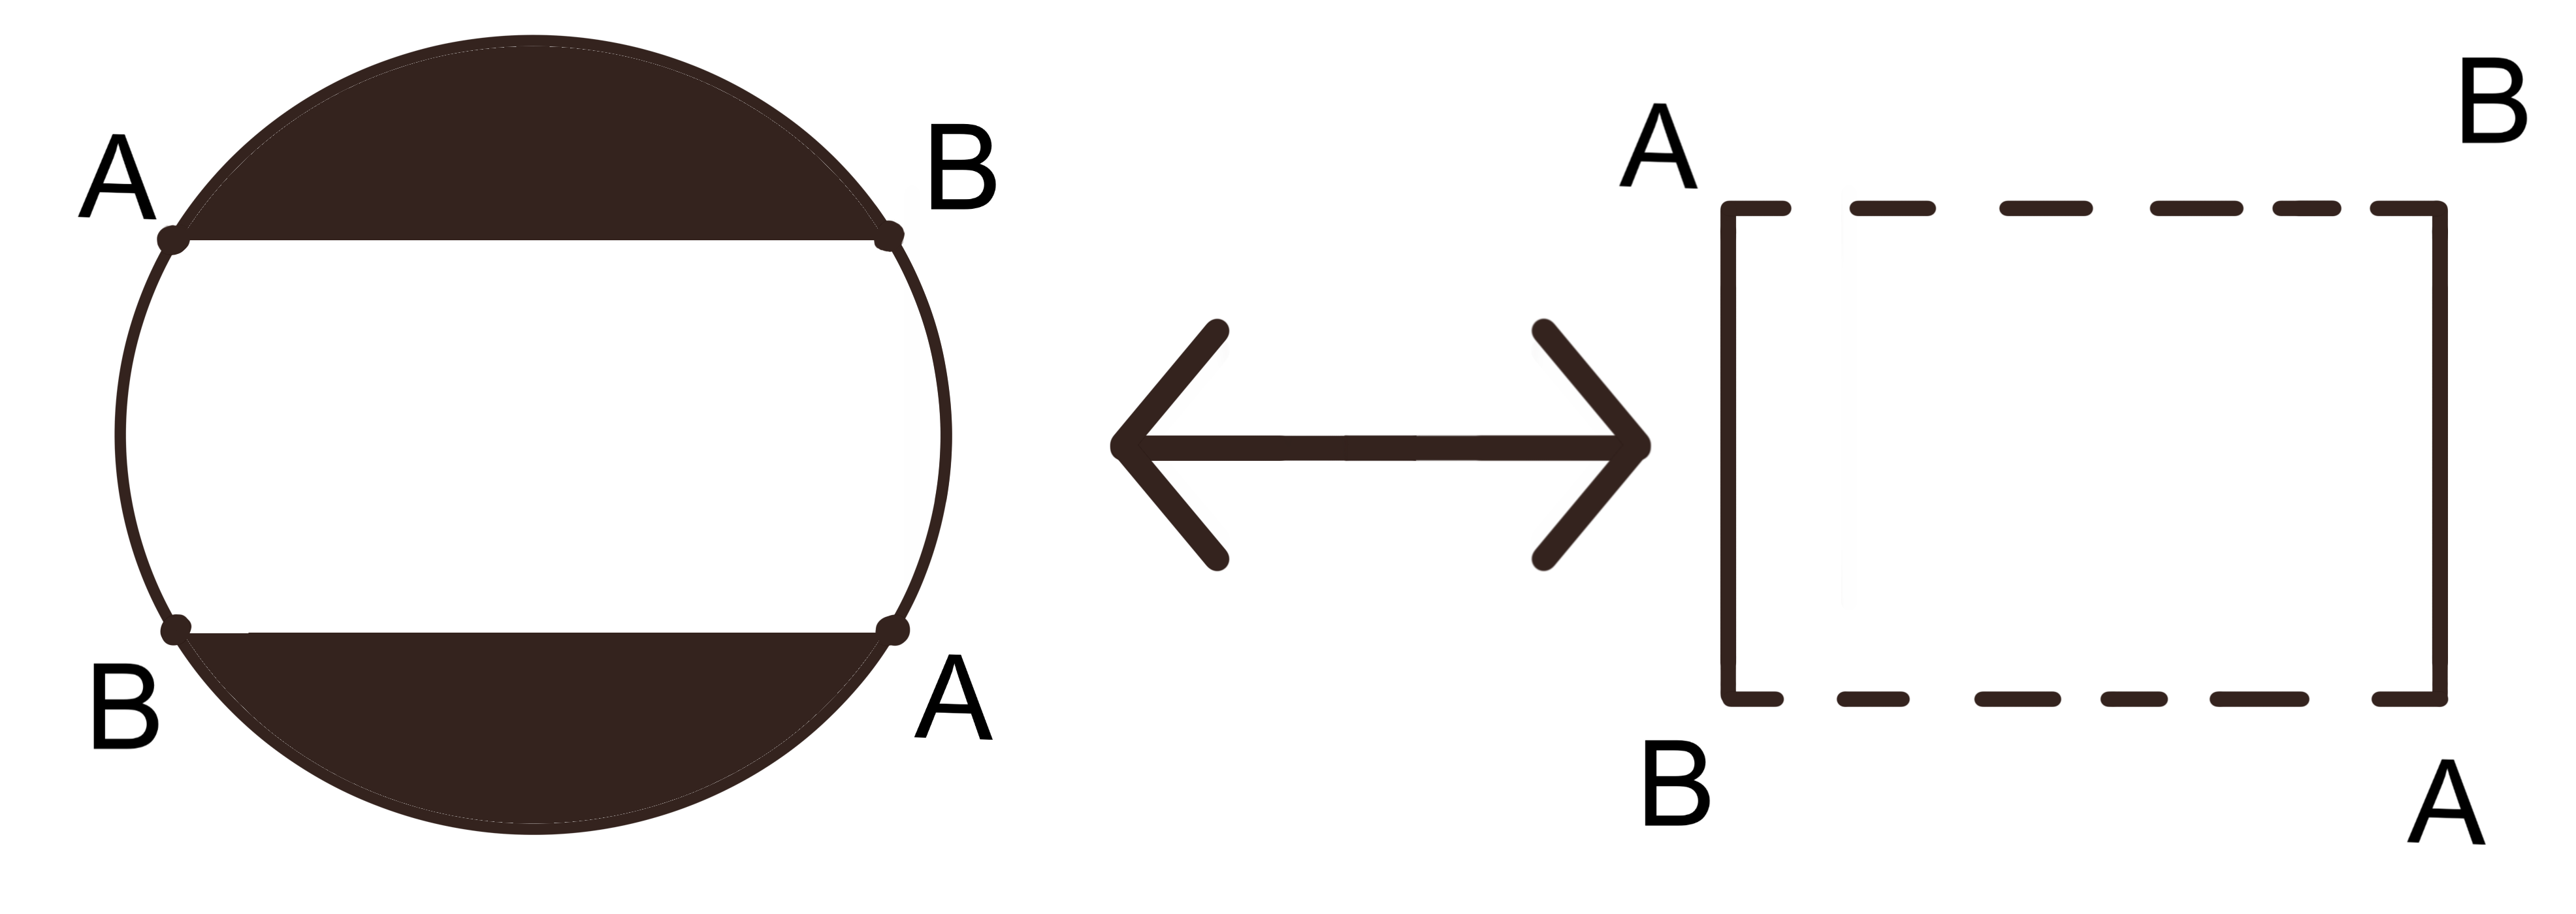
\includegraphics[width=0.4\linewidth]{imagenes/planop_sinD.png}
	\caption{Plano proyectivo menos un subconjunto homemorfo al disco cerrado}
	\label{fig:planop sin D}
\end{figure} 

\noindent Partiendo de dos planos proyectivos,  $I$ e $II$, retiramos el disco como en la figura \ref{fig:planop sin D}. Luego procedemos a identificar ambos conjuntos como se indica en la figura \ref{fig:sumaconexadeppsEnLema}.

\begin{figure}[h!]
	\centering
	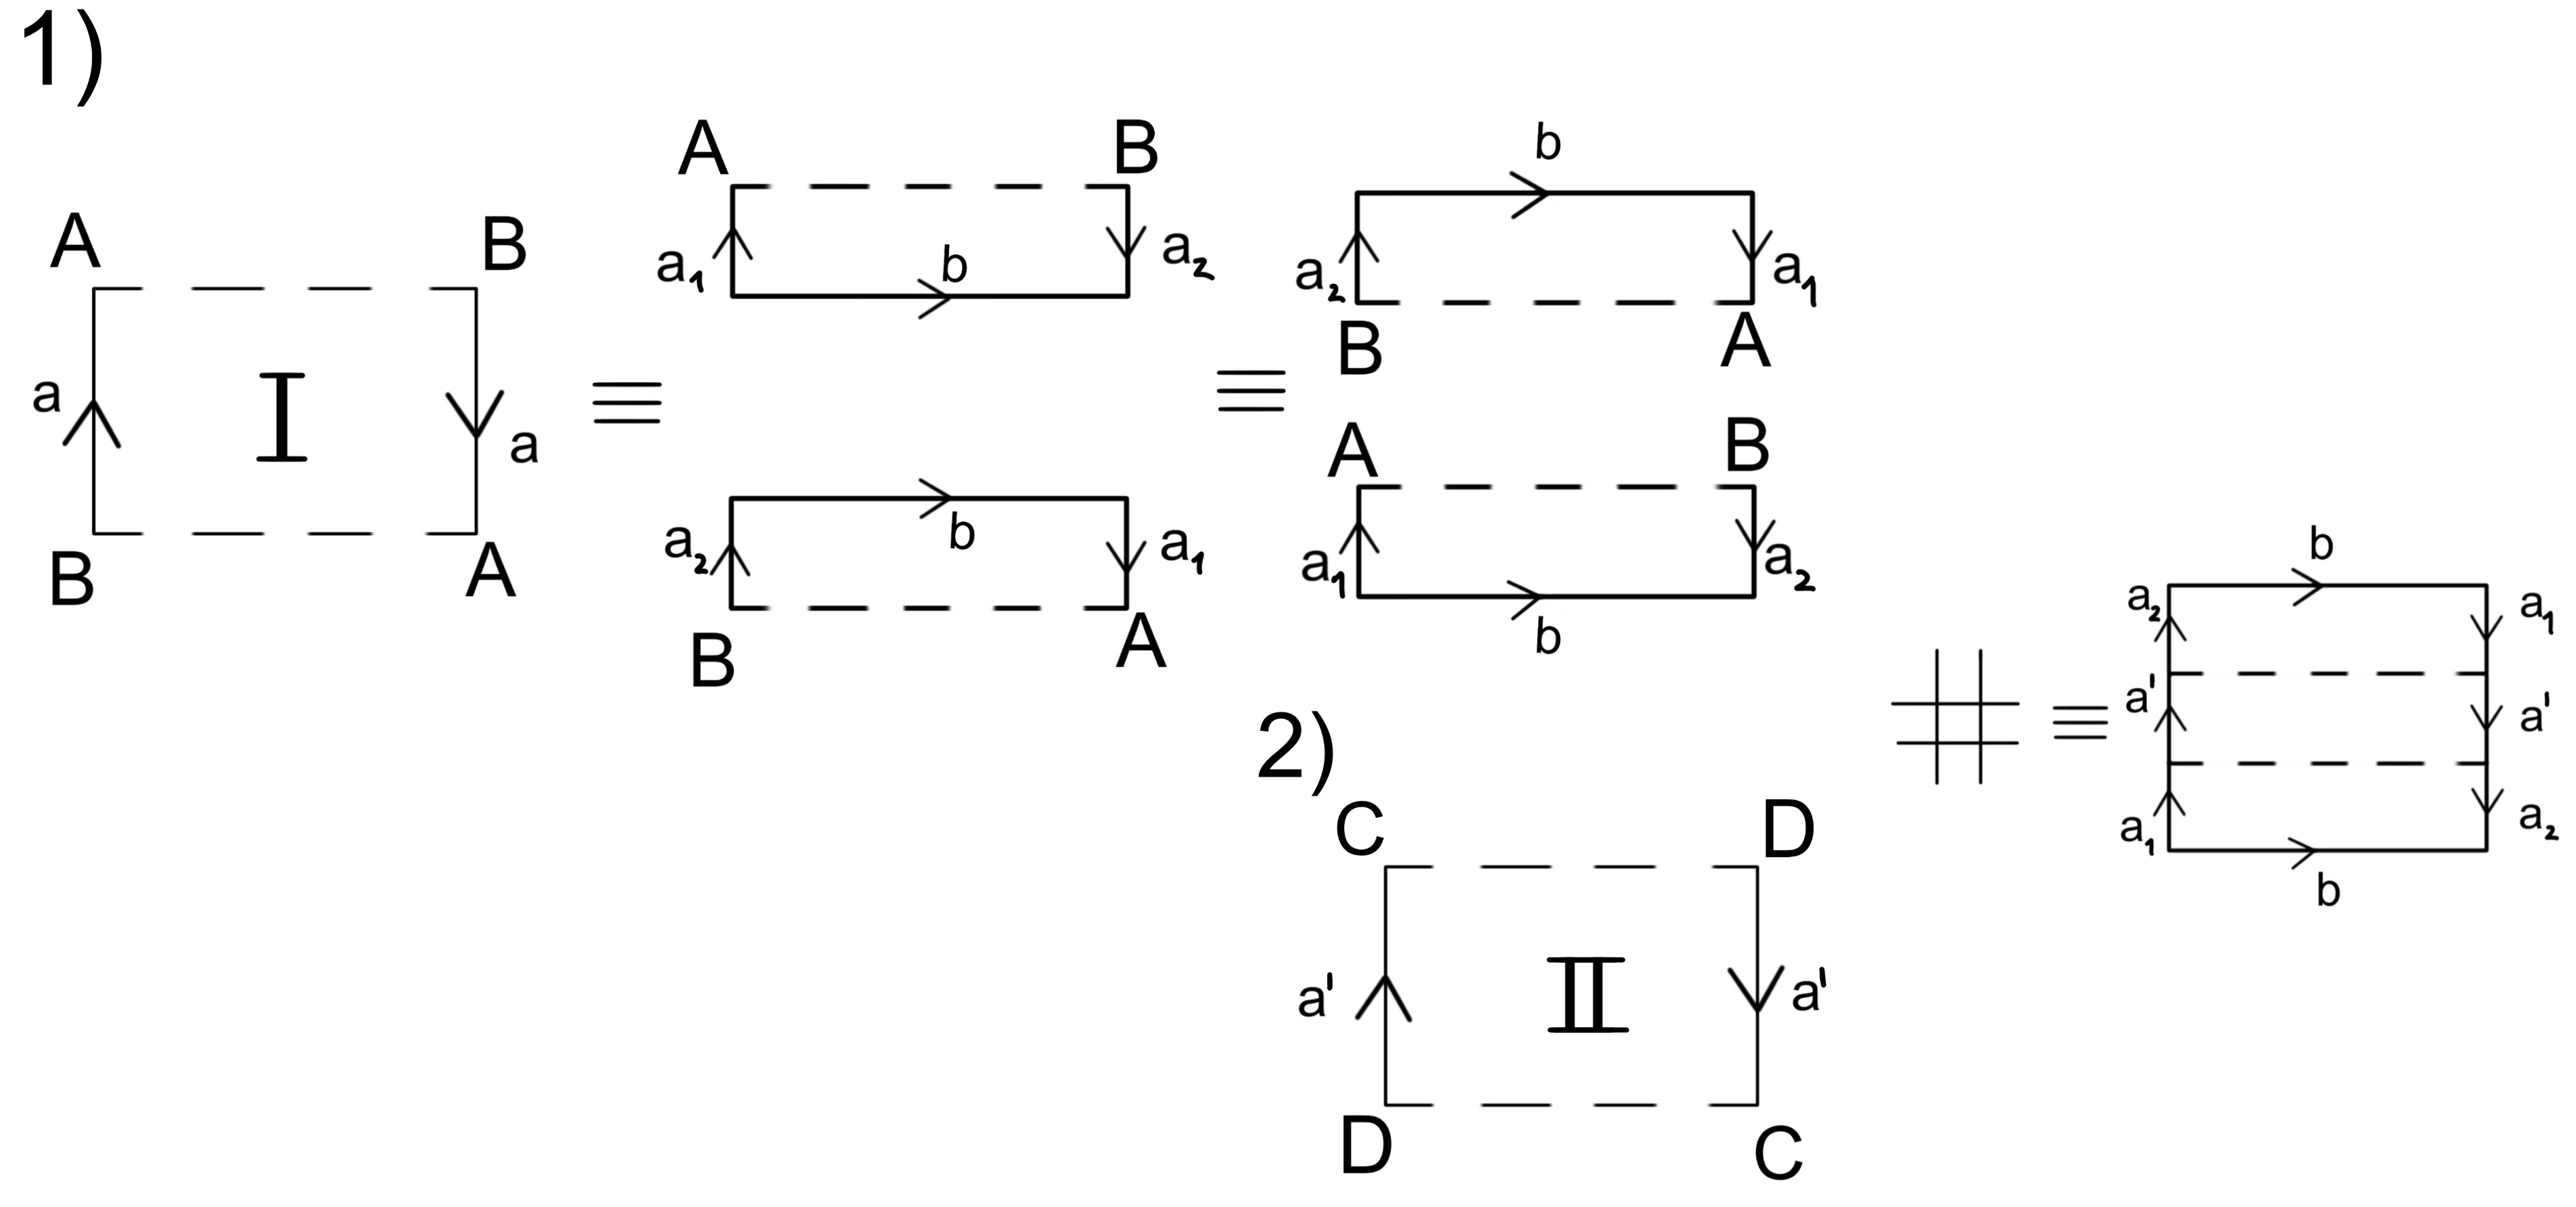
\includegraphics[width=0.8\linewidth]{imagenes/sumappsEnLema.png}
	\caption{Botella de Klein = $ I \# II$}
	\label{fig:sumaconexadeppsEnLema}
\end{figure} 

La figura final obtenida  es una Botella de Klein.
\end{proof}
\end{lema}

El ávido lector se habrá dado cuenta de un detalle de la demostración: ¡retirar un disco de un plano proyectivo lo convierte en una banda de M\"obius!


\section{Triangulación de una superficie}
\label{seccion de triangulacion}
Una triangulación, en caso de existir, pretende expresar una superficie como un conjunto de triángulos identificados por las aristas. La noción de triangulación, \textit{a priori} inofensiva, será un ingrediente clave para poder manipular superficies compactas. Se define rigurosamente como:

\begin{defin}\label{defin:triangulacion}
Una \textit{triangulación} de una superficie compacta $S$, consiste en un conjunto de cerrados, $\{T_1, ..., T_n\}$, que recubren a $S$ y en una familia de homeomorfismos, $\{\phi_1, ..., \phi_n\}$, que cumplen:

\begin{align*}
	\phi_i: T'_i \longrightarrow T_i
\end{align*}

Donde $T'_i$ es un triángulo del plano $\mathbb{R}^2$.
Además, se exige que para cualesquiera dos $T_i$ y $T_j$ con $i\neq j$, se cumpla una de las siguientes condiciones: o son conjuntos totalmente disjuntos; o comparten un vértice en común y solo eso; o tienen toda una arista en común y solo eso.\\
Adicionalmente, llamaremos \textit{vértice} a todo elemento de $S$ que se corresponde por algún $\phi_i$ con un vértice en el plano. Y llamaremos \textit{arista} a todo subconjunto de $S$ que tenga por imagen una arista de algún $T'_i$. A una superficie que admite una triangulación la llamaremos una superficie \textit{triangulable}.\\
\textbf{Observación:} La definición se puede extender para superficies no compactas si permitimos que el conjunto de triángulos sea numerables, y exigiendo que todo punto del conjunto tenga un entorno que interseque solo a un número finito de triángulos.
\end{defin}


Intuitivamente, podemos pensar en una triangulación como una teselación por triángulos de una superficie dada. Estudiemos algunos ejemplos concretos para familiarizarnos con el concepto:

El toro se puede triangular como ilustra la figura  \ref{fig:toro triangulado}. Fijémonos que basta con definir una lista de triángulos, con sus respectivos vértices, para concretar una trinagulación. En la figura indicada la lista de triángulos sería:

\begin{align*}
124 \quad 245 \quad 235 \quad 356 \quad 136 \quad 164 \\
457 \quad 578 \quad 568 \quad 689 \quad 469 \quad 497 \\
178 \quad 182 \quad 289 \quad 293 \quad 397 \quad 137 \\
\end{align*}

\begin{figure}[h!]
	\centering
	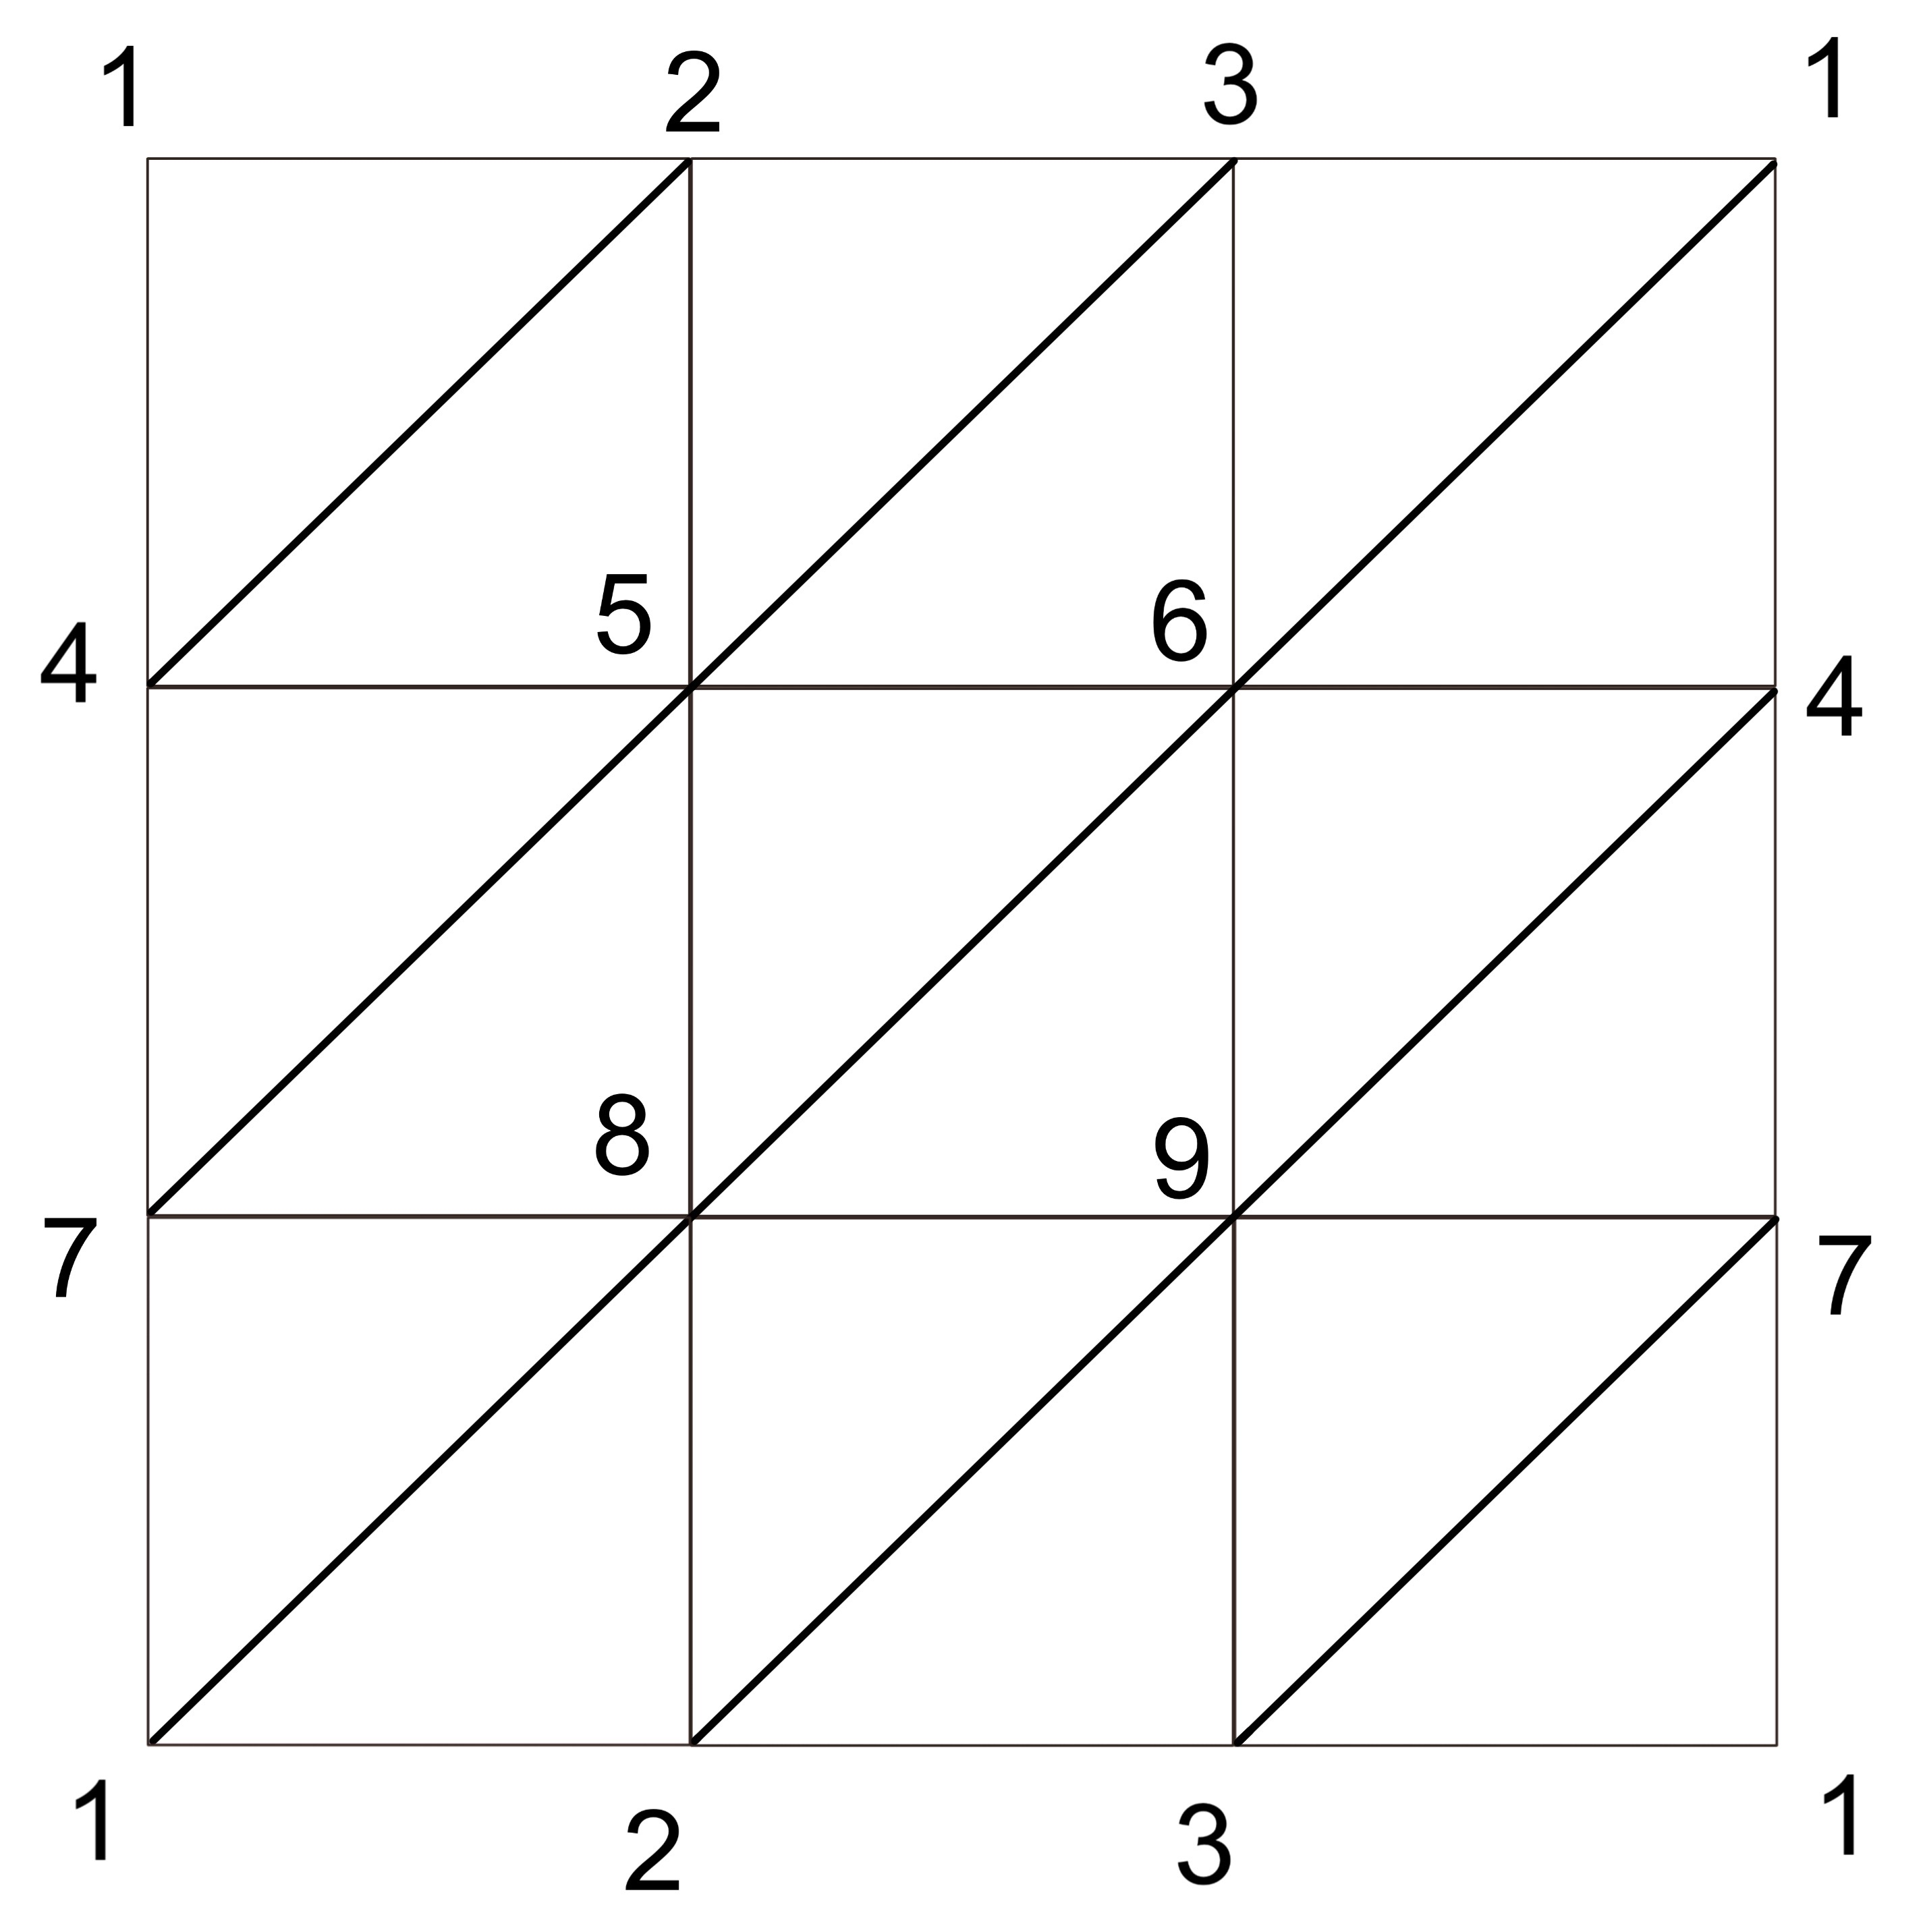
\includegraphics[width=0.3\linewidth]{imagenes/toro_triangulado.png}
	\caption{Triangulación del toro}
	\label{fig:toro triangulado}
\end{figure} 

En la figura \ref{fig:no triangulaciones} señalamos un par de intentos de simplificar la triangulación del toro. Sin embargo, notemos que ninguna de las dos imágenes son triangulación del toro. La primera, aunque satisface las condiciones de triangulación, no es homeomorfa al toro; La segunda ni siquiera satisface las condiciones.

\begin{figure}[h!]
	\centering
	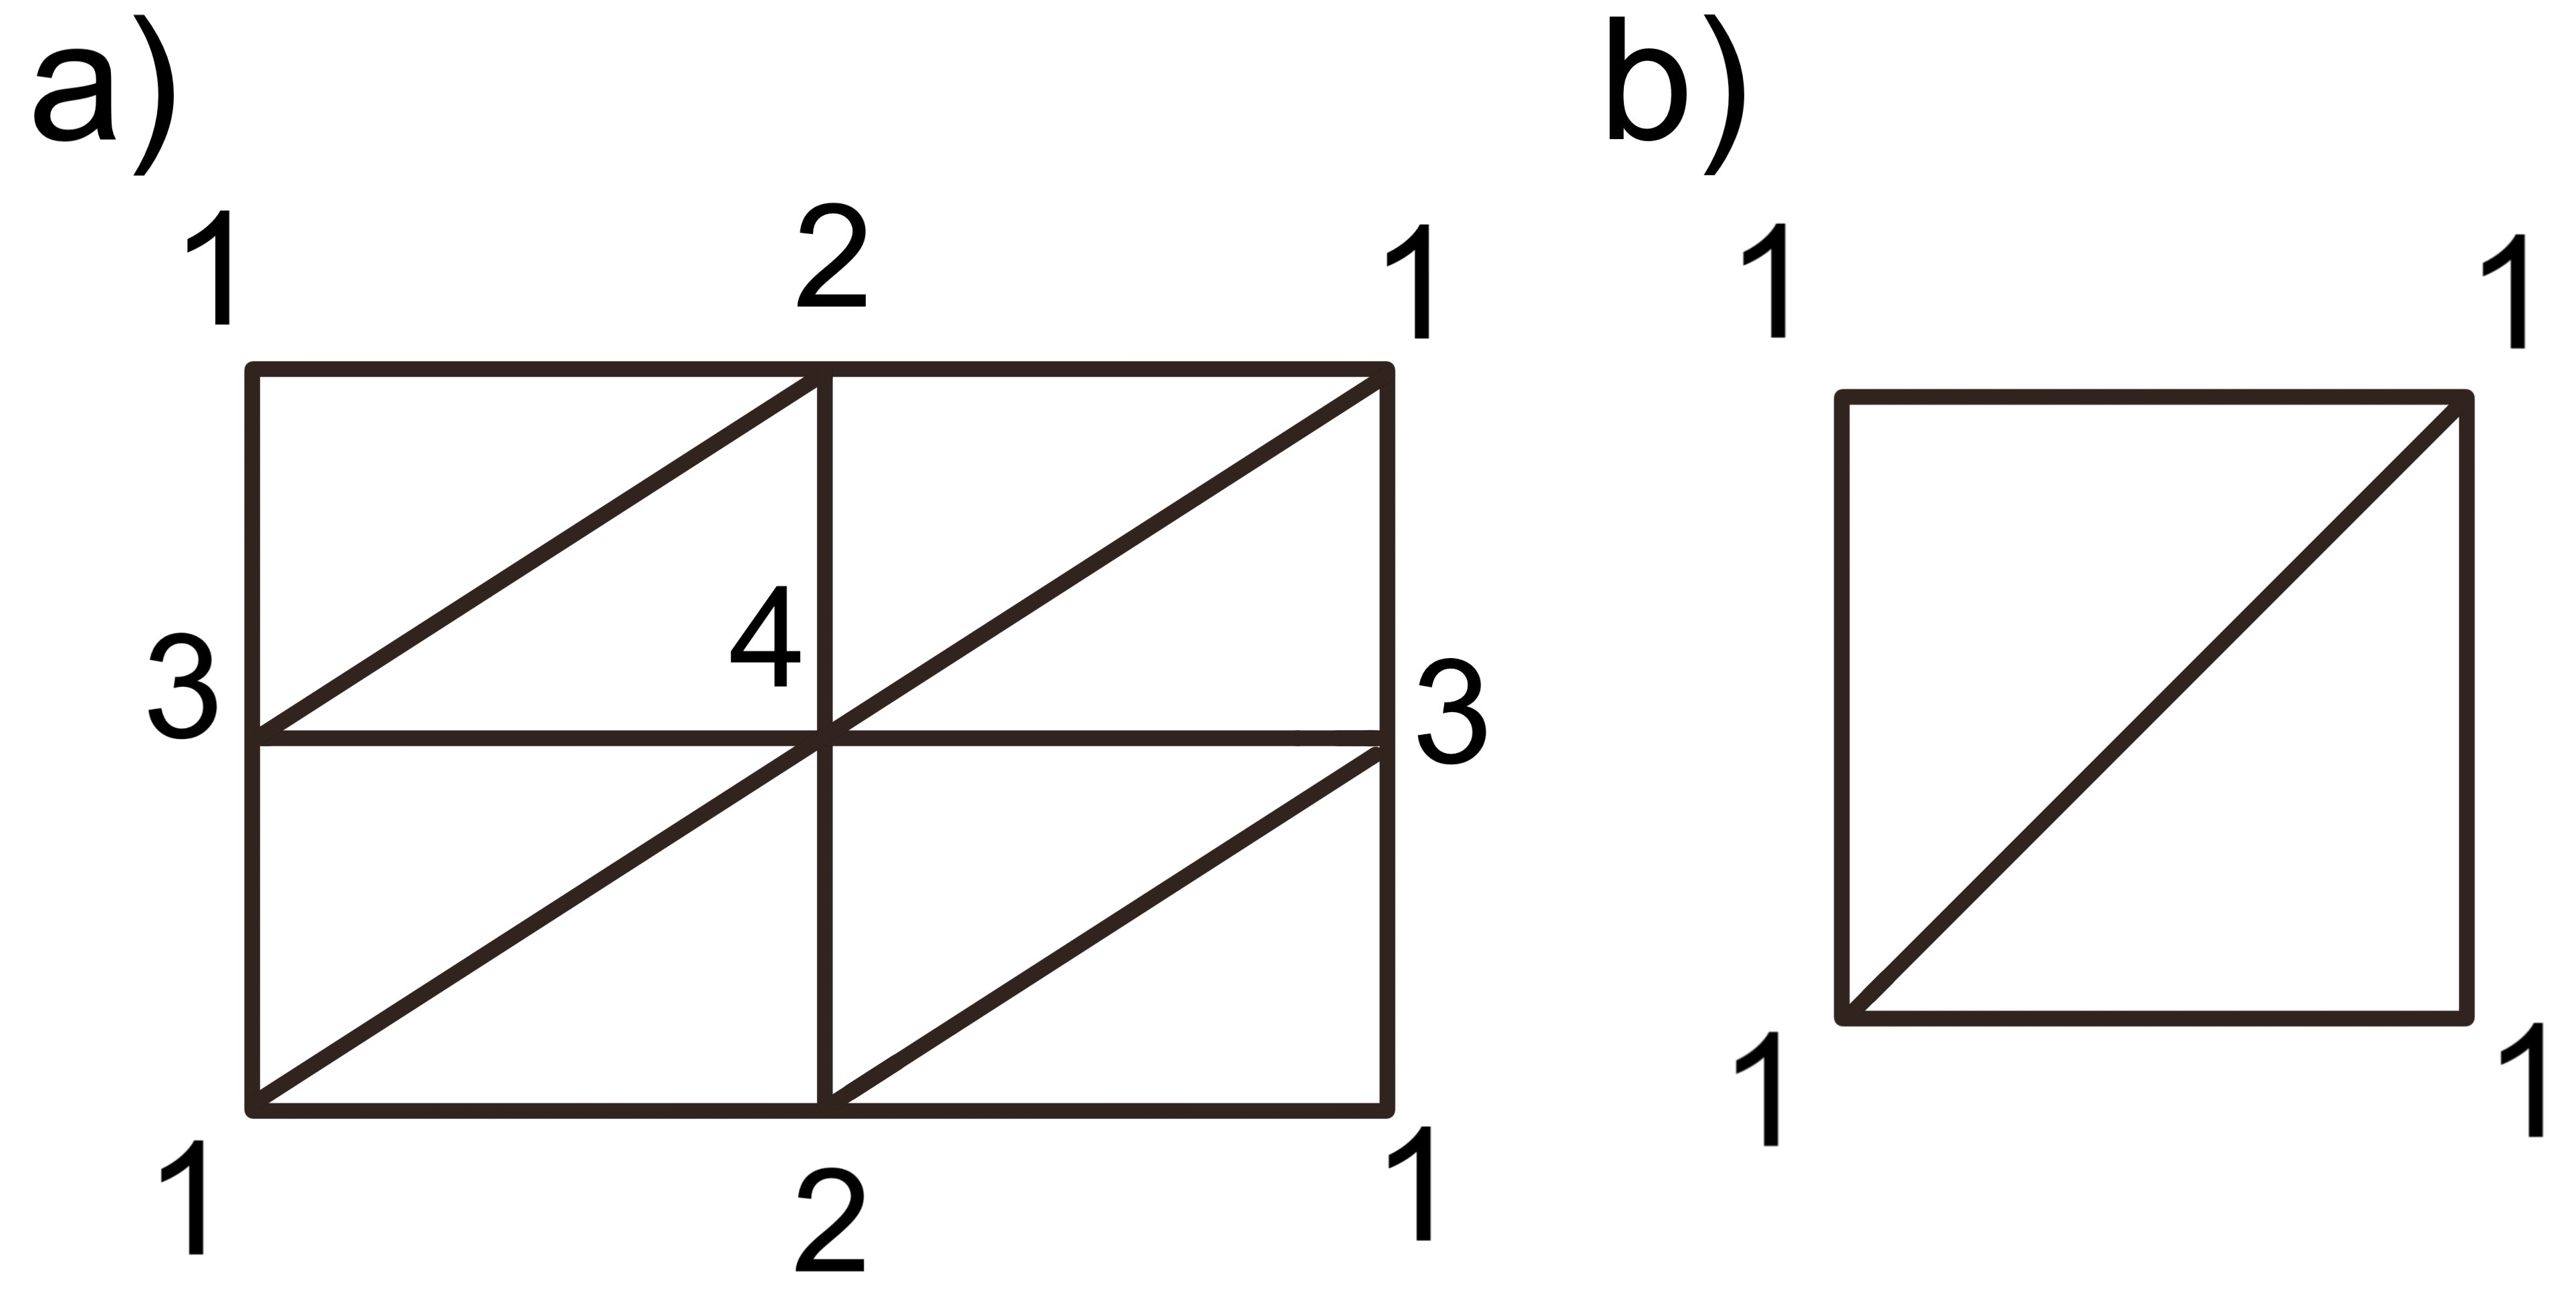
\includegraphics[width=0.5\linewidth]{imagenes/no_triangulaciones.png}
	\caption{Ejemplos de cosas que no son triangulaciones}
	
	\label{fig:no triangulaciones}
\end{figure} 

Para el caso del plano proyectivo, se propone en la figura \ref{fig:plano proyectivo triangulado} una triangulación.

\begin{figure}[h!]
	\centering
	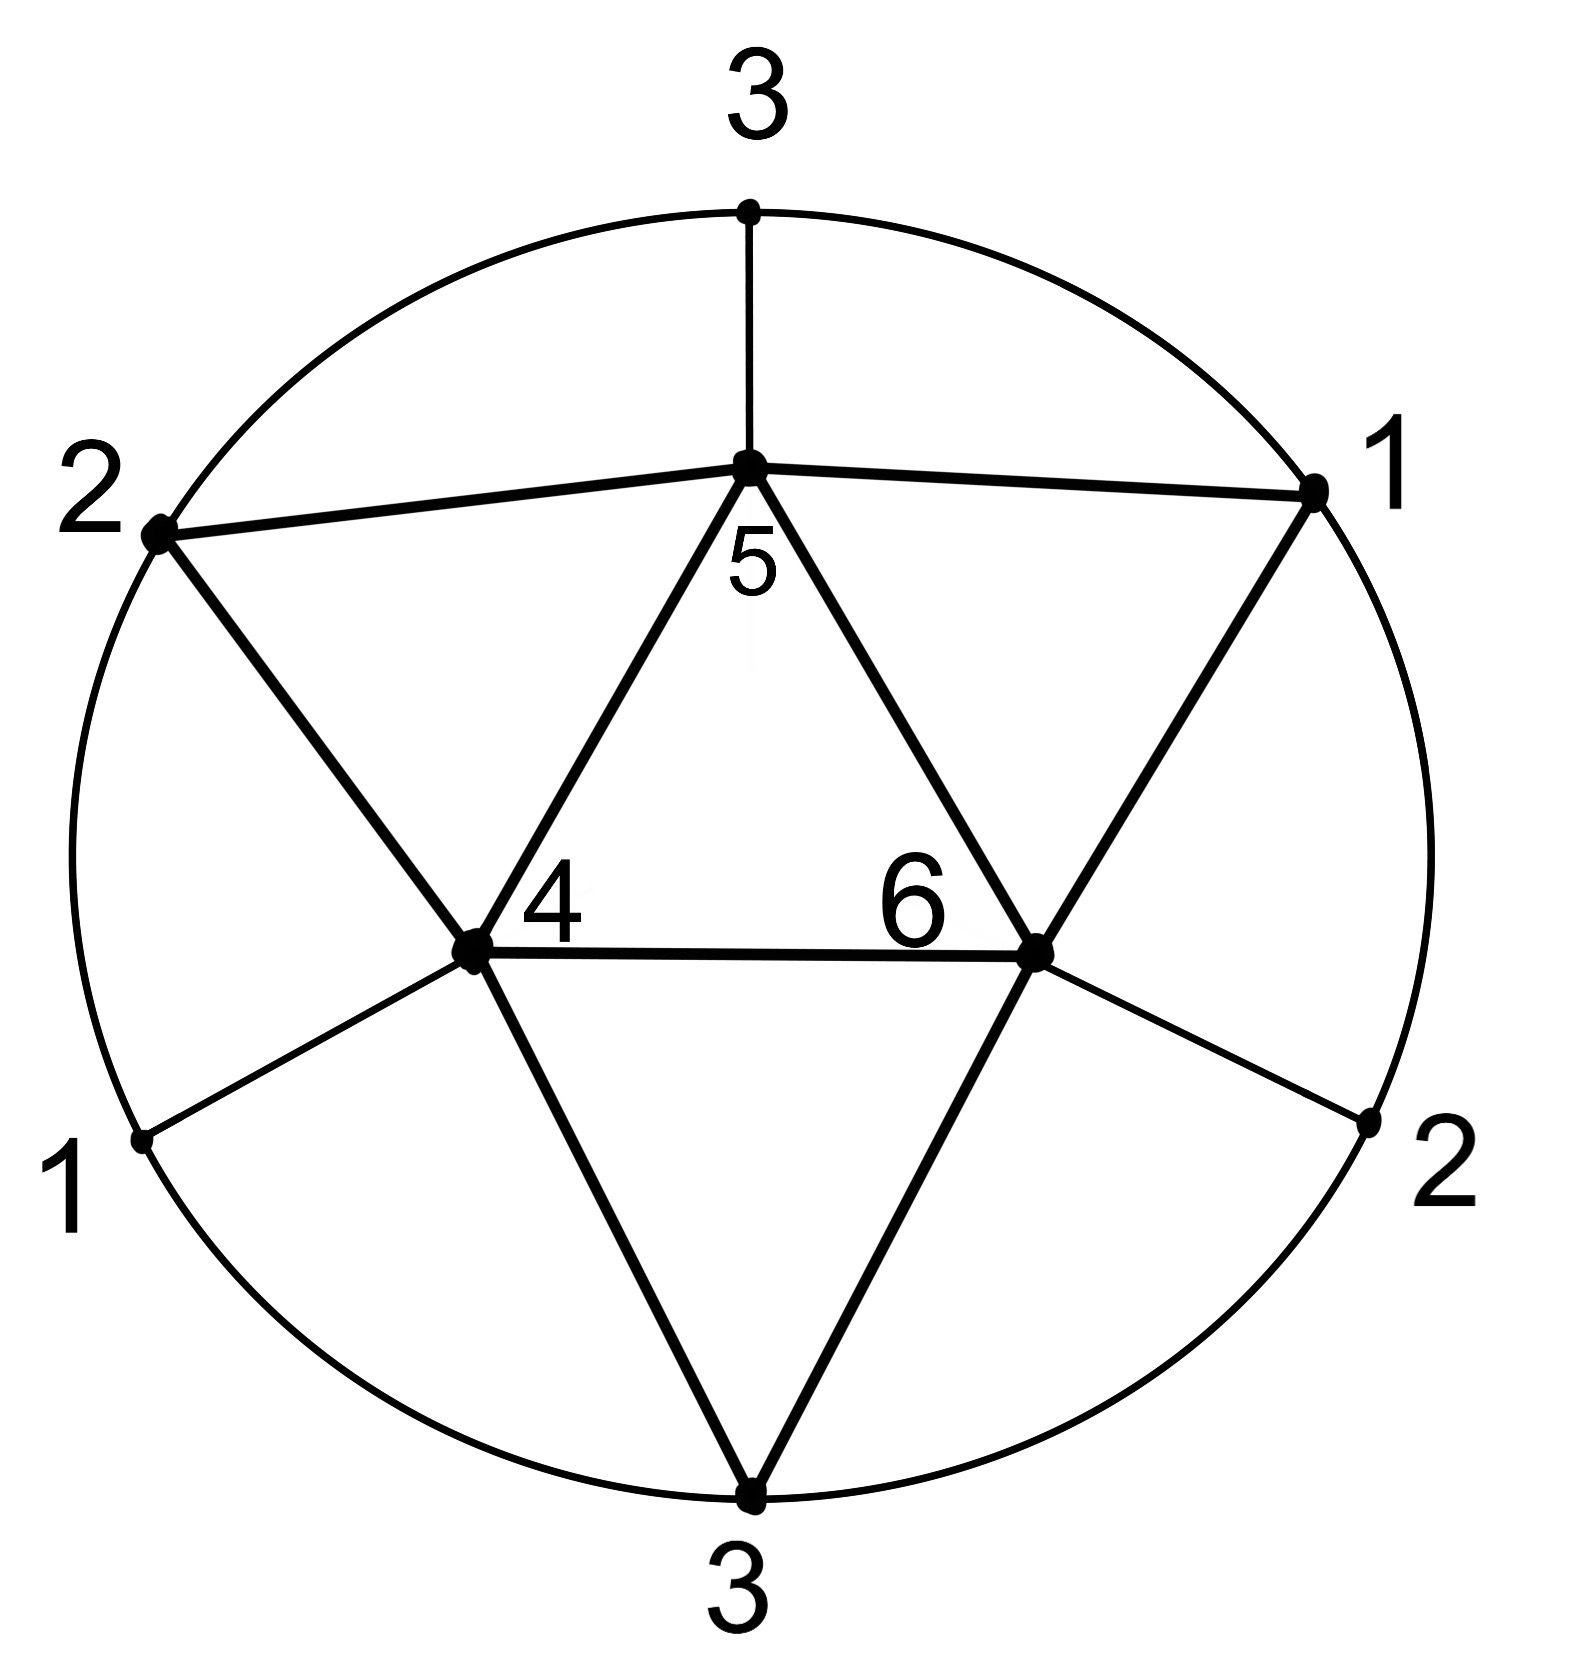
\includegraphics[width=0.3\linewidth]{imagenes/planop_triangulado.png}
	\caption{Triangulación del plano proyectivo}
	\label{fig:plano proyectivo triangulado}
\end{figure} 


\subsection*{Resultados sobre la triangulación}

Primero, veamos un par de lemas que nos enmarcan el comportamiento de las triangulaciones:

\begin{lema}\label{lema:lema1detriangulacion}
Sea $S$ una superficie triangulable entonces una arista lo es de exactamente dos triángulos.

\begin{proof}
Supongamos que una arista lo es de uno o más de dos triángulos. Elegimos un $x\in S$ de dicha arista. Por un lado, sabemos que un entorno de $x$ es homeomorfo a 
\[U^2 = \{x\in\reales^2: ||x||<1\}\]
Por otra parte, veamos los distintos casos:

\begin{enumerate}
\item[(a)] Si la arista lo fuese de un único triángulo, entonces tendríamos entornos de $x$ homeomorfos a
\[ H^2 = \{(x,y)\in\reales^2: x^2+y^2<1, \, y\geq 1 \} \]

\item[(b)] Si la arista lo fuese de  $n$ triángulos, con $n\geq 3$. Entonces tendríamos entornos de $x$ homeomorfos a pegar $n$ conjuntos de la forma de $H^2$ (podemos hacerlos disjuntos trasladándolos). Más rigurosamente, el conjunto a cocientar sería
\[
   \bigcup^n_{i=1} \{(x+10i,y)\in\reales^2: (x-10i)^2+y^2<1, \, y\geq 1 \} \}	        
\]
Identificando los puntos con $y=0$. En la figura \ref{fig:tripleplano} ilustramos el caso para $n=3$.
\end{enumerate}    

En cualquiera de los dos casos estaríamos incurriendo en un absurdo, con lo que concluimos la demostración.
\end{proof}
\end{lema}

\begin{figure}[h!]
	\centering
	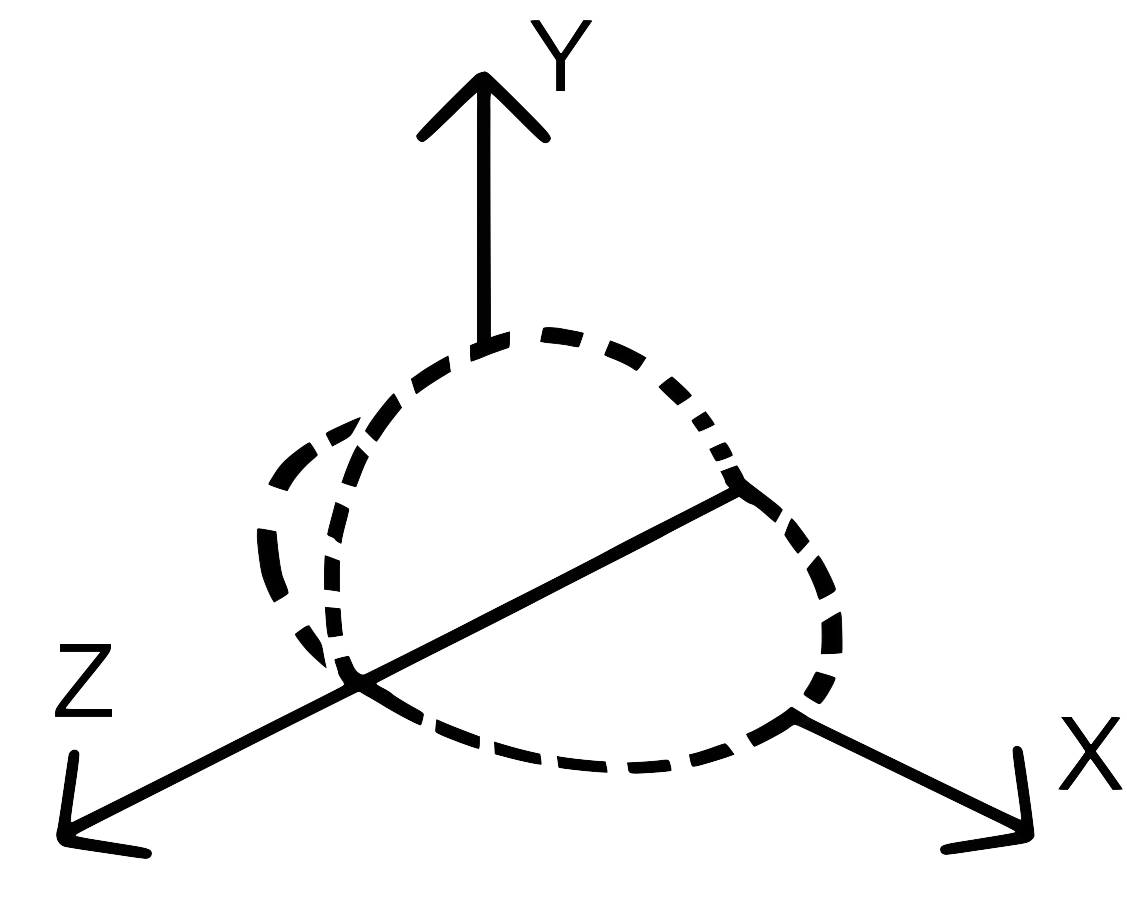
\includegraphics[width=0.4\linewidth]{imagenes/tripleplano.png}
	\caption{Identificación por la frontera de $H^2$}
	\label{fig:tripleplano}
\end{figure}

\begin{lema}\label{lema:lema2detriangulacion}
Sea  $S$ una superficie triangulable y $v\in S$ un vértice en esa triangulación, entonces podemos ordenar el conjunto de todos los triángulos con vértice $v$ cíclicamente,  $T_0, T_1, ..., T_n = T_0$, de manera que $T_i$ y $T_{i+1}$ tienen toda una arista en común para todo $0\leq i\leq n-1$.

\begin{proof}
Fijado un vértice $v$, podemos utilizar el lema anterior (\ref{lema:lema1detriangulacion}) para hacer una partición del conjunto de triángulos que tienen a $v$ por vértice. Si ocurriese que hay más de un conjunto disjunto en la partición, entonces $v$ no podría tener un entorno homeomorfo a $U^2$.
\end{proof}

\end{lema}

La idea de triangulación compone una herramienta potente para el manejo de superficies en general. Sin embargo, para usarla primero es necesario probar que de hecho existe  tal triangulación. Por suerte, el siguiente resultado del matemático Tibor Radó nos garantiza su existencia. Enunciamos el teorema sin, lamentablemente, dar la correspondiente demostración.

\begin{teor}{Teorema de triangulación}\label{teor:teoremaDeTriangulacion}	

Toda superficie separable es triangulable.
\end{teor}
En el contexto de este trabajo, las superficies son segundo numerables por definición. Por tanto, todas las superficies son separables y con ello triangulables.

Con este teorema concluimos el arsenal de herramientas que nos hará falta para emprender la demostración del teorema de clasificación de superficies compactas.





\chapter{Clasificación de superficies compactas}
\label{chap:clasifcompacta}
\begin{teor}{Teorema de clasificación de superficies compactas}\label{teor:teoremadeclasificacion}	

Toda superficie compacta es homeomorfa a una esfera, a una suma conexa de toros o una suma conexa de planos proyectivos.
\end{teor}

\subsubsection*{Idea de la demostración}
El primer paso de la demostración será probar que podemos tratar cualquier superficie compacta como un polígono en $\reales^2$ con sus aristas identificadas a pares. Para esta parte de la demostración nos serviremos del teorema \ref{teor:teoremaDeTriangulacion} de \textit{T. Radó}.\\
Posteriormente, utilizando la representación en $\reales^2$, iremos modificando la figura con transformaciones homeomorfas. Cada transformación supondrá una simplificación del polígono obtenido. Tras aplicar todos los pasos, comprobaremos que el polígono final se corresponde con una de las expresiones canónicas introducidas en la sección \ref{subsec:expresionescanonicassumasconexas}. Para completar la demostración necesitaremos del siguiente lema (en el anexo adjuntamos la demostración de este resultado \ref{anexo:lema1}):
\begin{lema}\label{lema:planop+toro=3planop}
La suma conexa de un toro y un plano proyectivo es homeomorfa a la suma conexa de tres planos proyectivos.
\end{lema}
Una vez obtenidas las expresiones canónicas de \ref{subsec:expresionescanonicassumasconexas}, habremos concluido que la superficie inicial es homeomorfa o a una esfera, o a una suma conexa de toros, o a una suma conexa de planos proyectivos.\\

\section{Primer paso}
\label{seccion primer paso}
Buscamos demostrar que cualquier superficie compacta $S$ es homeomorfa a un polígono en $\reales^2$ con sus aristas identificadas a pares.

Por el teorema \ref{teor:teoremaDeTriangulacion} tenemos que $S$ es triangulable. Sean $T_1, T_2, ..., T_n$ los triángulos de S y sean $T'_1, T'_2, ...,  T'_n$ los correspondientes triángulos en $\reales^2$, tenemos los homeomorfismos:
\[ \phi_i: T'_i \longrightarrow T_i \]
Podemos asumir que los $T'_i$ son disjuntos (en caso de que no lo fueran, bastaría componerlos con una traslación). Además, podemos organizar los triángulos de tal forma que todo $T_i$ tenga al menos una arista $e_i$ en común con algún triángulo $T_1, ..., T_{i-1}$ para $2\leq i \leq n$. Elegiremos $T_2$ con una arista en común con $T_1$, $T_3$ con una arista en común con $T_1$ o $T_2$, y así sucesivamente. Nótese que si en algún punto no pudiésemos elegir un $T_k$, tendríamos entonces dos conjuntos disjuntos $\{T_1, ..., T_{k-1} \}$ y $\{T_k, ..., T_n\}$, pero esto dividiría a $S$ en dos conjuntos cerrados disjuntos contradiciendo la hipótesis de conexión.\\
Sea $T' = \bigcup T'_i$, definimos la función 
\[ \phi: T' \longrightarrow S \]
como $\phi |_{T'_i} = \phi_i$ para todo $i$. La función $\phi$ es sobreyectiva y continua (la continuidad se prueba escribiendo cualquier abierto en $S$ como unión finita de la partición de triángulos). Al ser $T'$ compacto y $S$ Hausdorff, entonces $\phi$ es cerrada, de lo que se sigue que $S$ tiene la topología cociente inducida por $\phi$.

El polígono que queremos construir será descrito como espacio cociente de $T'$. Por hipótesis, tenemos que $e_i$ es arista de los triángulos $T_i$ y $T_j$ para algún $1\leq j < i$, y a su vez $\phi^{-1}(e_i)$ es arista de $T'_i$ y $T'_j$. Identificamos ambos triángulos en $T'$ a lo largo de la arista $\phi^{-1}(e_i)$. El mismo procedimiento se puede aplicar para las aristas $e_2, e_3, ..., e_n$, obteniendo como resultado un conjunto cociente $D$ del conjunto inicial $T'$. La función $\phi$ induce una nueva función continua $\psi: D \longrightarrow S$. De nuevo, al ser $D$ compacto y $S$ Hausdorff, tenemos que $\psi$ es   cerrada y con ello que $S$ tiene la topología cociente inducida por esta función. \\
Veamos que $D$ es homeomorfo al disco cerrado $E^2 = \{x\in \reales^2: ||x||\leq 1\}$:

\begin{enumerate}
\item[(a)] Tenemos que el triángulo $T'_i$ en $\reales^2$ es homeomorfo a $E^2$.

\item[(b)] Dados dos discos cerrados $E^2_1$ y $E^2_2$, si los identificamos por un segmento cerrado de sus fronteras, obtenemos un espacio cociente homeomorfo, de nuevo, a un disco cerrado. De aquí se sigue que, si tenemos dos triángulos $T'_i$ y $T'_j$  identificados por una de sus aristas, entonces el espacio resultante es homeomorfo a $E^2$.
\end{enumerate}
Utilizando (a) y (b) tenemos que el espacio cociente $D$ obtenido a partir de $T'$, es topológicamente equivalente a un disco cerrado. Además, sabemos que el espacio cociente que induce $\psi$ coincidirá  con el disco cerrado en el cual segmentos de su frontera están identificados a pares; esto se sigue del proceso de construcción de $D$, teniendo en cuenta que al identificar la arista $\phi^{-1}(e_i)$ de dos triángulos, el resto de aristas en la frontera siguen emparejadas (sabemos que van por parejas por el lema \ref{lema:lema1detriangulacion}).


En la figura \ref{fig:tetraedrotriangulado} tenemos un tetraedro triangulado.

\begin{figure}[h!]
	\centering
	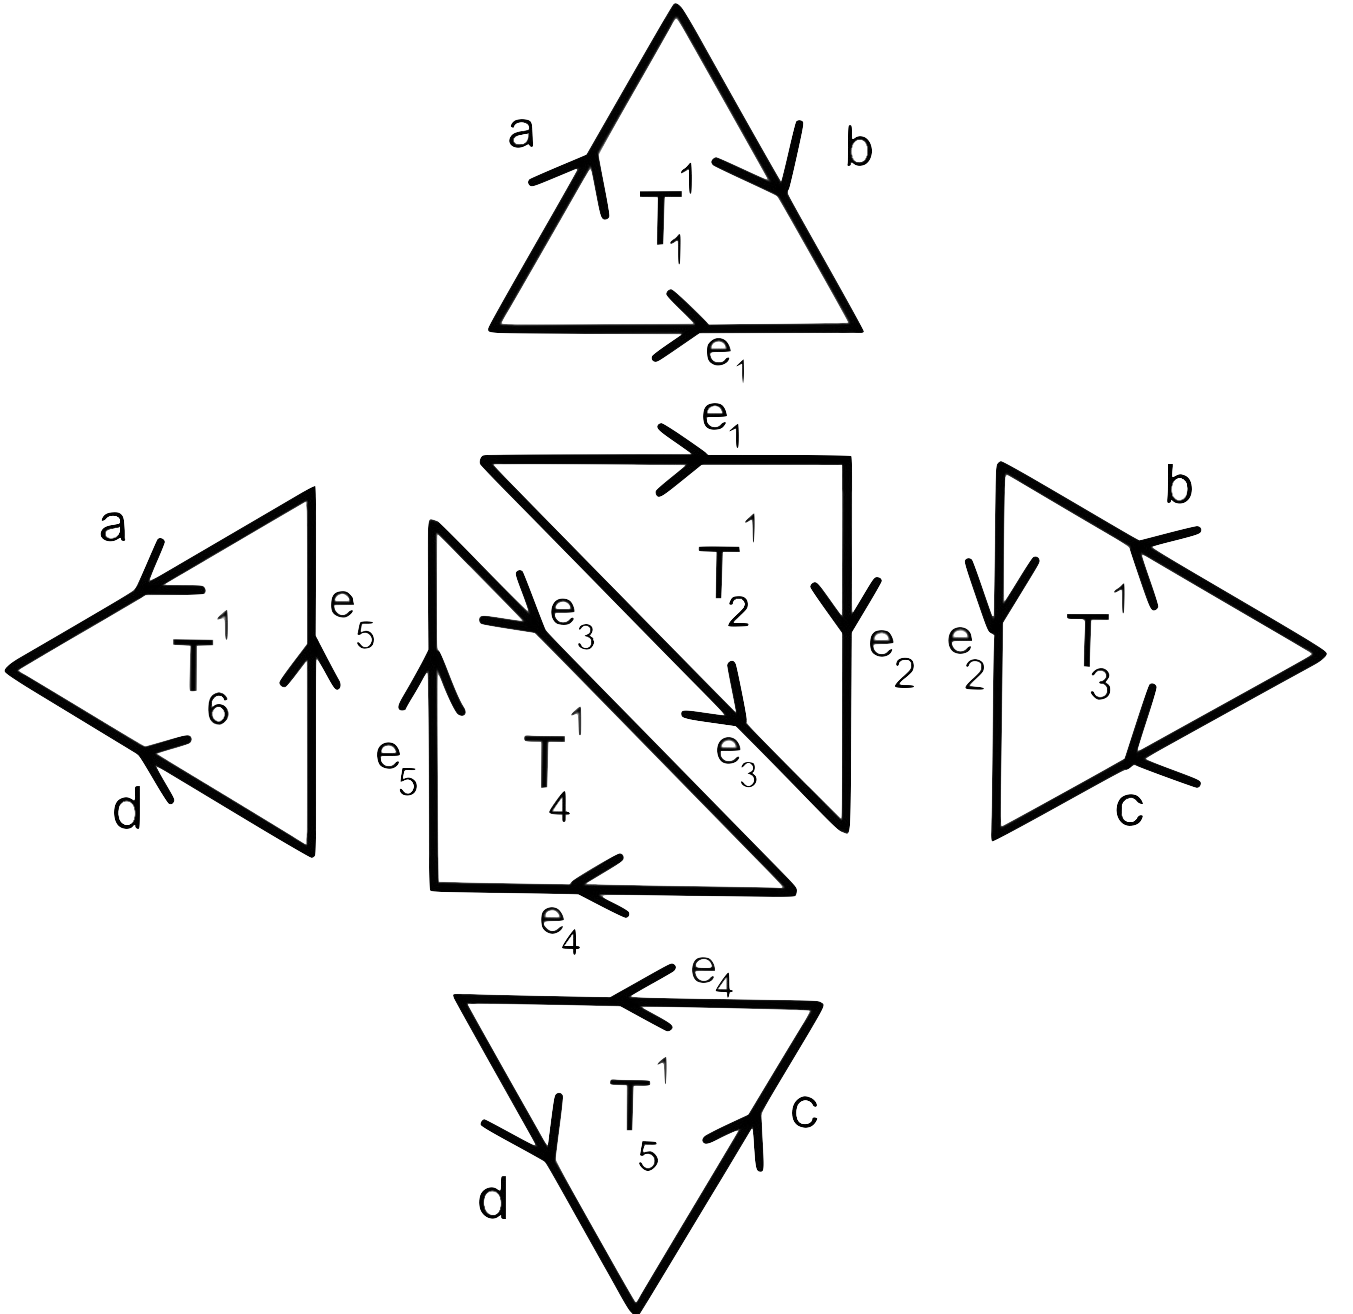
\includegraphics[width=0.3\linewidth]{imagenes/tetraedro.png}
	\caption{Tetraedro triangulado}
	\label{fig:tetraedrotriangulado}
\end{figure}

Ilustramos en la figura \ref{fig:d} cómo se representaría el mismo tetraedro como el espacio cociente $D$ descrito en esta sección.

\begin{figure}[h!]
	\centering
	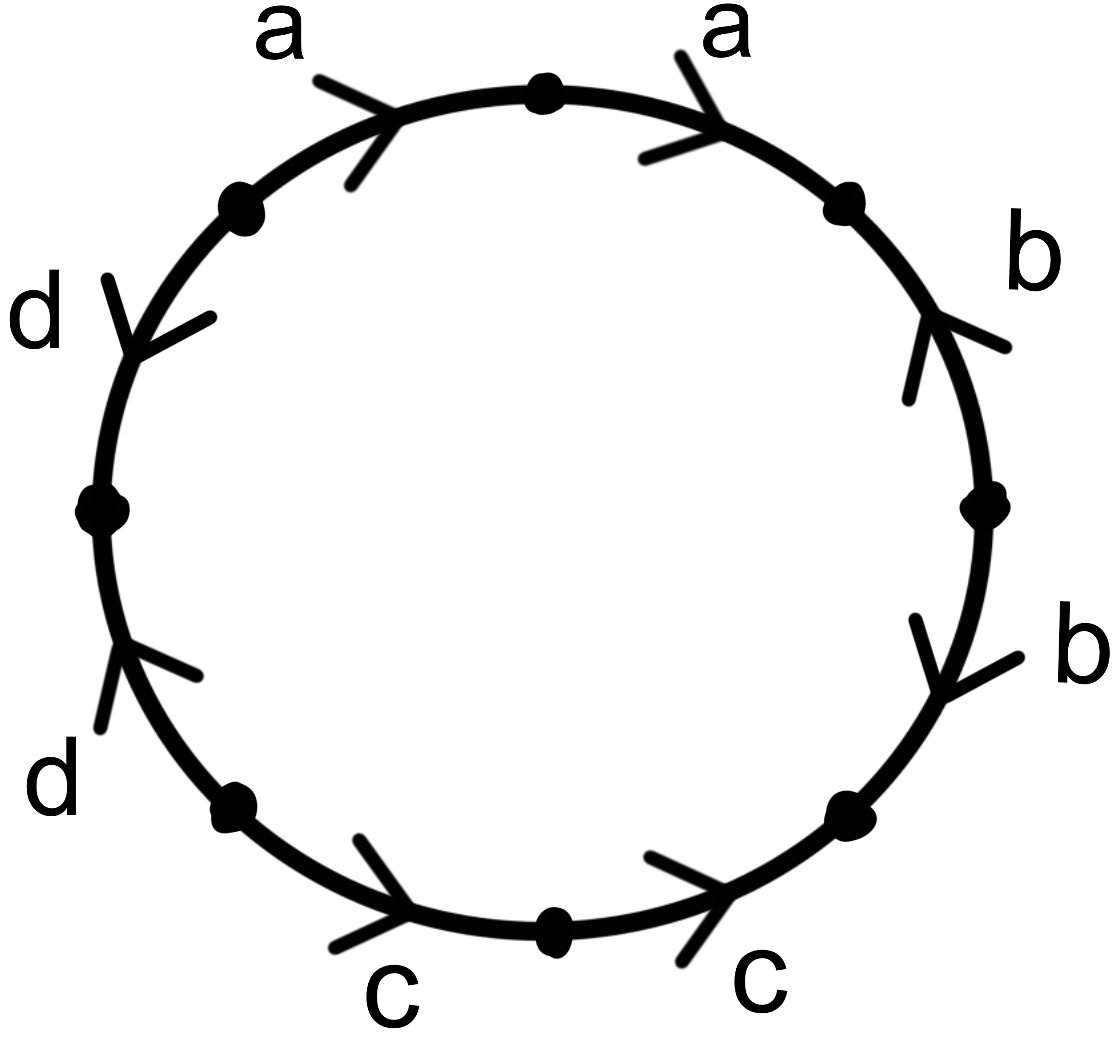
\includegraphics[width=0.3\linewidth]{imagenes/d.jpeg}
	\caption{Tetraedro como espacio cociente de un disco}
	\label{fig:d}
\end{figure}

A partir de aquí, manipularemos la superficie compacta $S$ como si de un polígono se tratase. Asumiendo que las aristas del polígono están identificadas a pares y sin ningún orden ni dirección particular.


\section{Segundo paso}

El segundo paso consiste en la eliminación de aristas adyacentes de primera especie.

Del primer paso hemos obtenido el polígono $D$ que representa a la superficie $S$ si se identifican sus aristas a pares. El polígono identificado lo podemos expresar con la misma notación que usamos para las expresiones canónicas (véase la sección \ref{subsec:expresionescanonicassumasconexas}). Por ejemplo, en el caso de la figura \ref{fig:d}, la expresión canónica sería:
\[ a^{-1}abb^{-1}cc^{-1}d^{-1}d \]
Si en esta expresión un par de aristas con el mismo símbolo aparecen  con exponentes +1 y -1 ($...a...a^{-1}$, por ejemplo), entonces diremos que el par es de \textit{primera especie}. Si aparecen ambas con el exponente +1, o ambas con -1, diremos que el par es de \textit{segunda especie}. En el caso de la figura \ref{fig:d} tenemos que los cuatro pares de aristas son de primera especie y, además, adyacentes.

En este paso buscaremos eliminar las aristas adyacentes de primera especie, i.e, con la forma $aa^{-1}$ o $a^{-1}a$. Suponiendo que el polígono tenga al menos 4 lados, la figura \ref{fig:paso2} indica cómo podríamos eliminar esta arista de nuestra expresión. El mismo procedimiento se sigue aplicando mientras haya aristas adyacentes de primer orden ó hasta que la expresión tenga únicamente dos aristas. En este último caso, tenemos que la expresión será $aa$ o $aa^{-1}$, es decir, homeomorfo a una esfera o a un plano proyectivo (véase la sección \ref{subsec:expcanonica}). En caso de que haya más de dos aristas y no queden aristas de primera especie se continúa al siguiente paso.
\begin{figure}[h!]
	\centering
	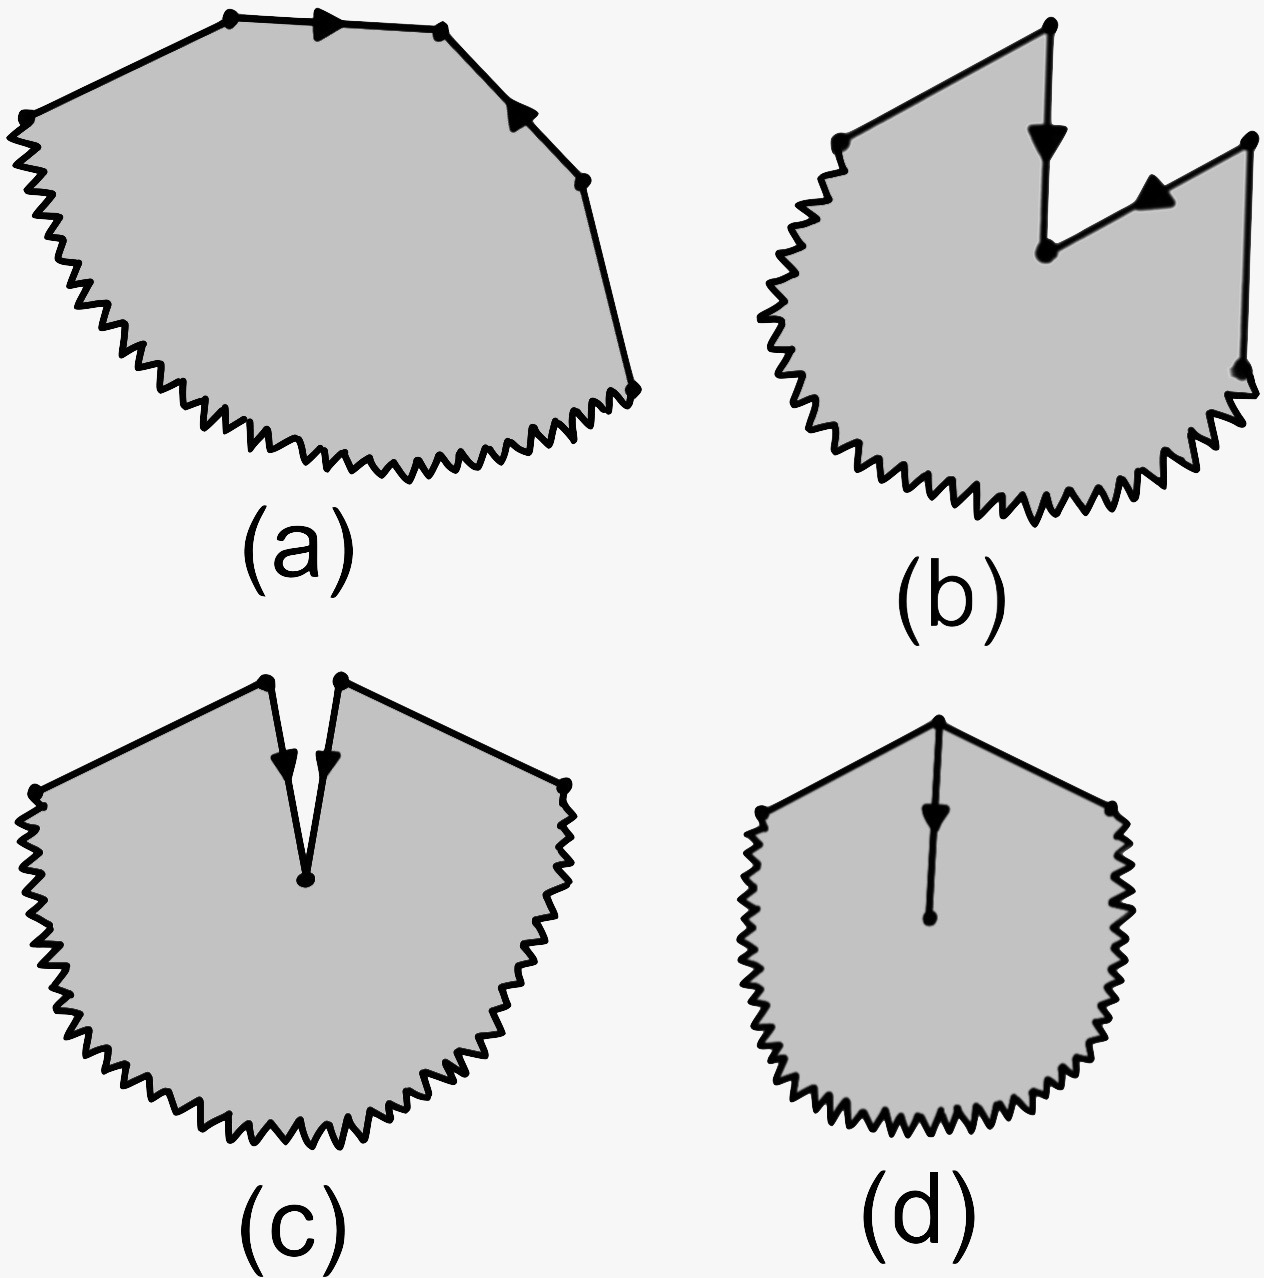
\includegraphics[width=0.4\linewidth]{imagenes/paso2.jpeg}
	\caption{Eliminando adyacencias de primera especie}
	\label{fig:paso2}
\end{figure}

\section{Tercer paso}

En este paso procederemos a transformar el polígono $D$, obtenido del paso anterior, para que todos sus vértices estén identificados entre sí, es decir, buscamos que todos los vértices representen el mismo punto en la superficie $S$. 

Podemos dividir los vértices en clases de equivalencia según qué vértices están identificados. Supongamos que al menos hay dos clases de equivalencias e intentemos eliminar una de ellas.\\
Como hay dos clases de equivalencia, entonces existen al menos dos vértices adyacentes $P$ y $Q$ que no pertenecen a la misma clase. En la figura\ref{fig:paso3} se ilustra el procedimiento. Sabemos que $a$ y $b$ no pueden estar identificados (no puede ser par de primera especie porque ya hemos aplicado el segundo paso, y no puede ser par de segunda especie porque los vértices son distintos), entonces cortamos e identificamos a lo largo de la línea $c$ tal y como  se muestra la figura. Al finalizar la transformación, tenemos un vértice menos de la clase $P$ y uno más de la clase $Q$. Una vez eliminado el vértice, se aplica el segundo paso nuevamente de ser posible y se repite el procedimiento. Tras un número finito de pasos habremos eliminado la clase de equivalencia de $P$. Iteramos de forma análoga hasta que tengamos una única clase de equivalencia de vértices del polígono.

\begin{figure}[h!]
	\centering
	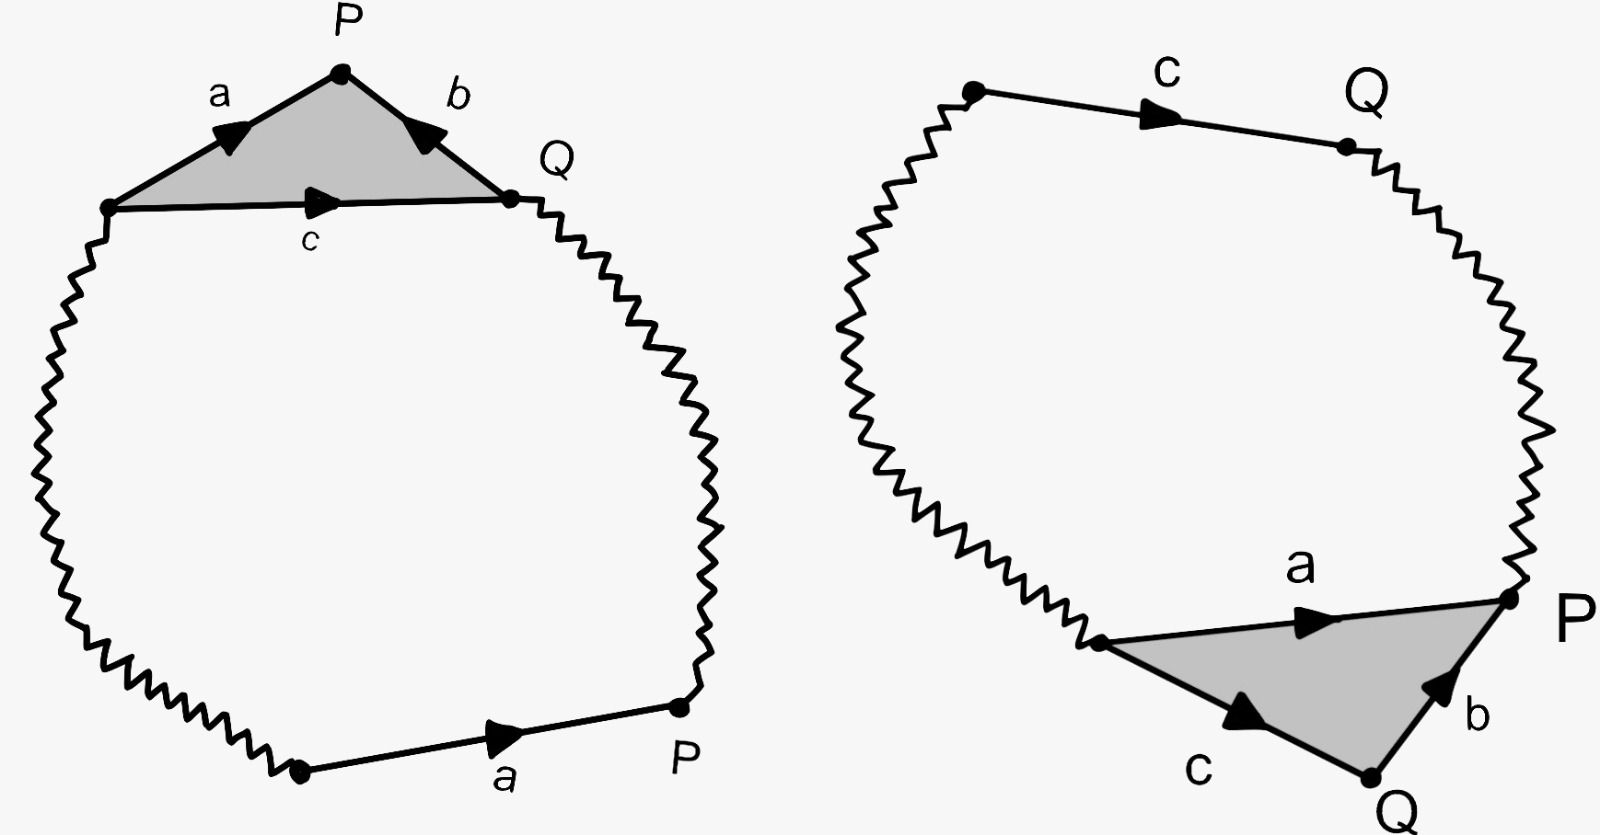
\includegraphics[width=0.4\linewidth]{imagenes/paso3.jpeg}
	\caption{Reduciendo clases de equivalencia de vértices}
	\label{fig:paso3}
\end{figure}


\section{Cuarto paso}

Ahora buscaremos hacer adyacentes todos los pares de aristas de segunda especie.

En la figura \ref{fig:paso4} ilustramos el proceso. Partimos de que tenemos dos aristas $b$ de segunda especie no adyacentes, y procedemos a cortar e identificar a través de $a$. Como resultado, hemos cambiado un par no adyacente a uno adyacente. Repetimos el mismo procedimiento hasta que todas las aristas de segunda especie sean adyacentes.

\begin{figure}[h!]
	\centering
	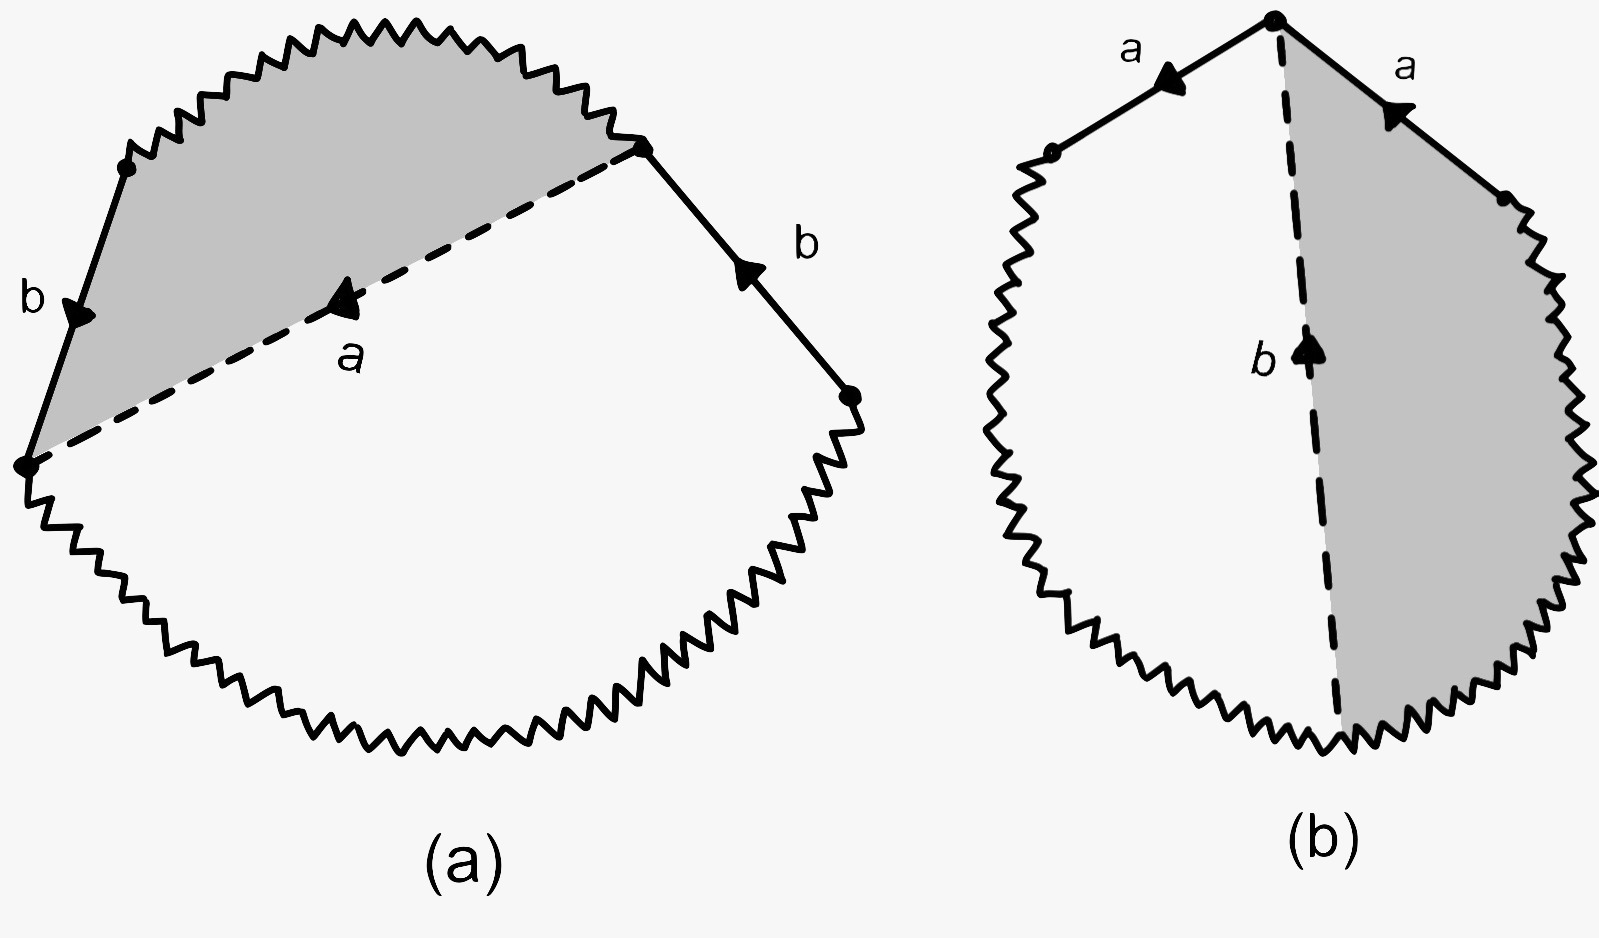
\includegraphics[width=0.4\linewidth]{imagenes/paso4.jpeg}
	\caption{Transformando en adyacentes aristas de segunda especie}
	\label{fig:paso4}
\end{figure}

En caso de no haber ninguna arista de primera especie, tendremos unas expresión de la forma $a_1a_1a_2a_2...a_na_n$, con lo que concluimos que la superficies es homeomorfa a la suma conexa de $n$ planos proyectivos (véase \ref{subsec:expresionescanonicassumasconexas}).

En caso de haber un par de  aristas de primera especie, denotémosla por $c$, probaremos que necesariamente existe otro par de primera especie que las intercala. En otras palabras, necesariamente existe otro par de aristas de primera especie, $d$, tal que la expresión obtenida es de la forma $c...d...c^{-1}...d^{-1}...$

\begin{figure}[h!]
	\centering
	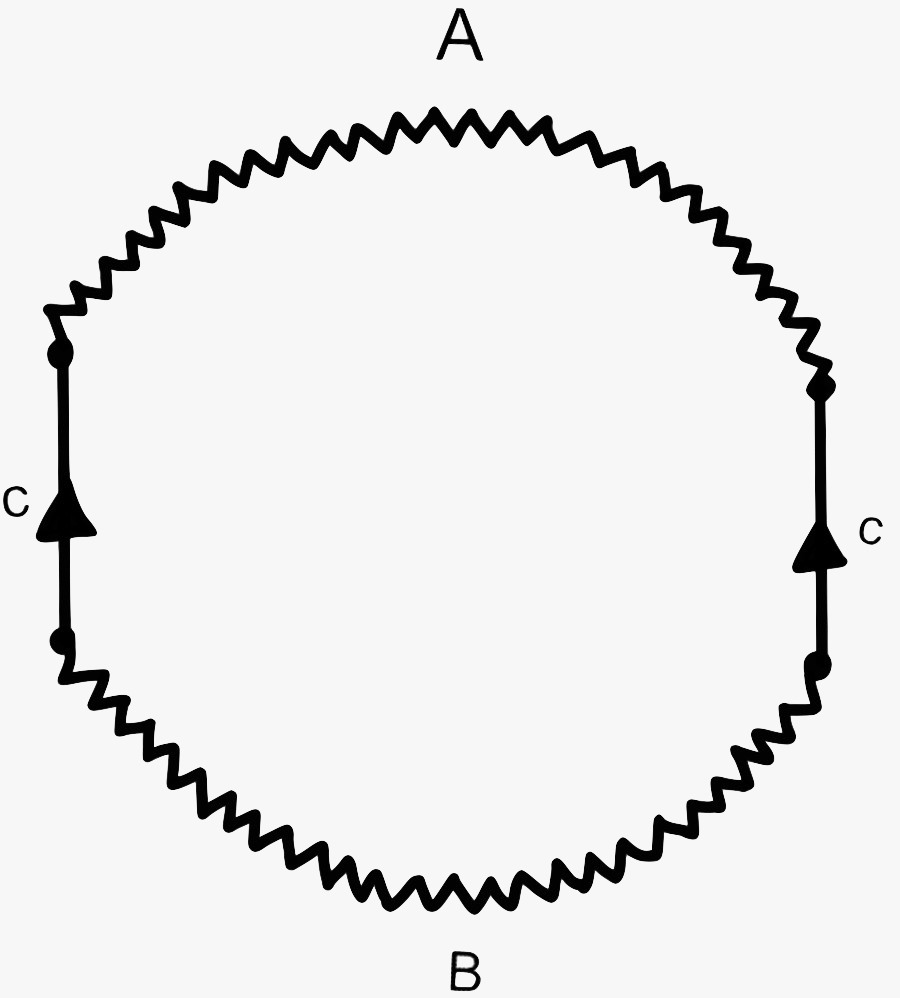
\includegraphics[width=0.2\linewidth]{imagenes/paso4_2.jpeg}
	\caption{Par de primera especie tras el paso 4}
	\label{fig:paso4_2}
\end{figure}

Para probar esto, supongamos que no existe el par $d$. Bajo este supuesto, el aspecto del polígono $D$ sería similar a \ref{fig:paso4_2}, donde A y B son ambas sucesiones de aristas. Por el cuarto paso, todas las aristas de segunda especie son adyacentes, con lo que, bajo el supuesto de que no exista $d$, no existiría ninguna arista de A identificada con una de B, ni viceversa. Sin embargo, ello implicaría que los vértices finales e iniciales de la arista $c$ no están identificados\footnote{El lema \ref{lema:lema2detriangulacion} nos permite crear un argumento por contradicción: Si hubiera algún vértice identificado en A y B, entonces podríamos identificar un par de aristas de este vértice entre sendas sucesiones (pero esto no ocurre por hipótesis).},  incurriendo así en una contradicción con el tercer paso.


\section{Quinto paso}

En este paso haremos adyacentes los pares de aristas de primera especie que estén intercalados como se indica en el paso anterior.

Supongamos que nuestro polígono tiene la expresión $a \ldots b \ldots a^{-1} \ldots b^{-1}$ (véase la figura \ref{fig:paso5} $(a)$). Primero, cortamos a lo largo de $c$ y pegamos las aristas $b$, obteniendo la figura \ref{fig:paso5} $(b)$.  Seguidamente, cortamos a lo largo de $d$ y pegamos $c$, con lo que obtenemos la figura \ref{fig:paso5} $(c)$. Nótese que hemos transformado nuestra expresión cambiando los pares $a$ y $b$, por $cdc^{-1}d^{-1}$.  De los pasos se sigue que los vértices siguen manteniendo una única clase de equivalencia.

\begin{figure}[h!]
	\centering
	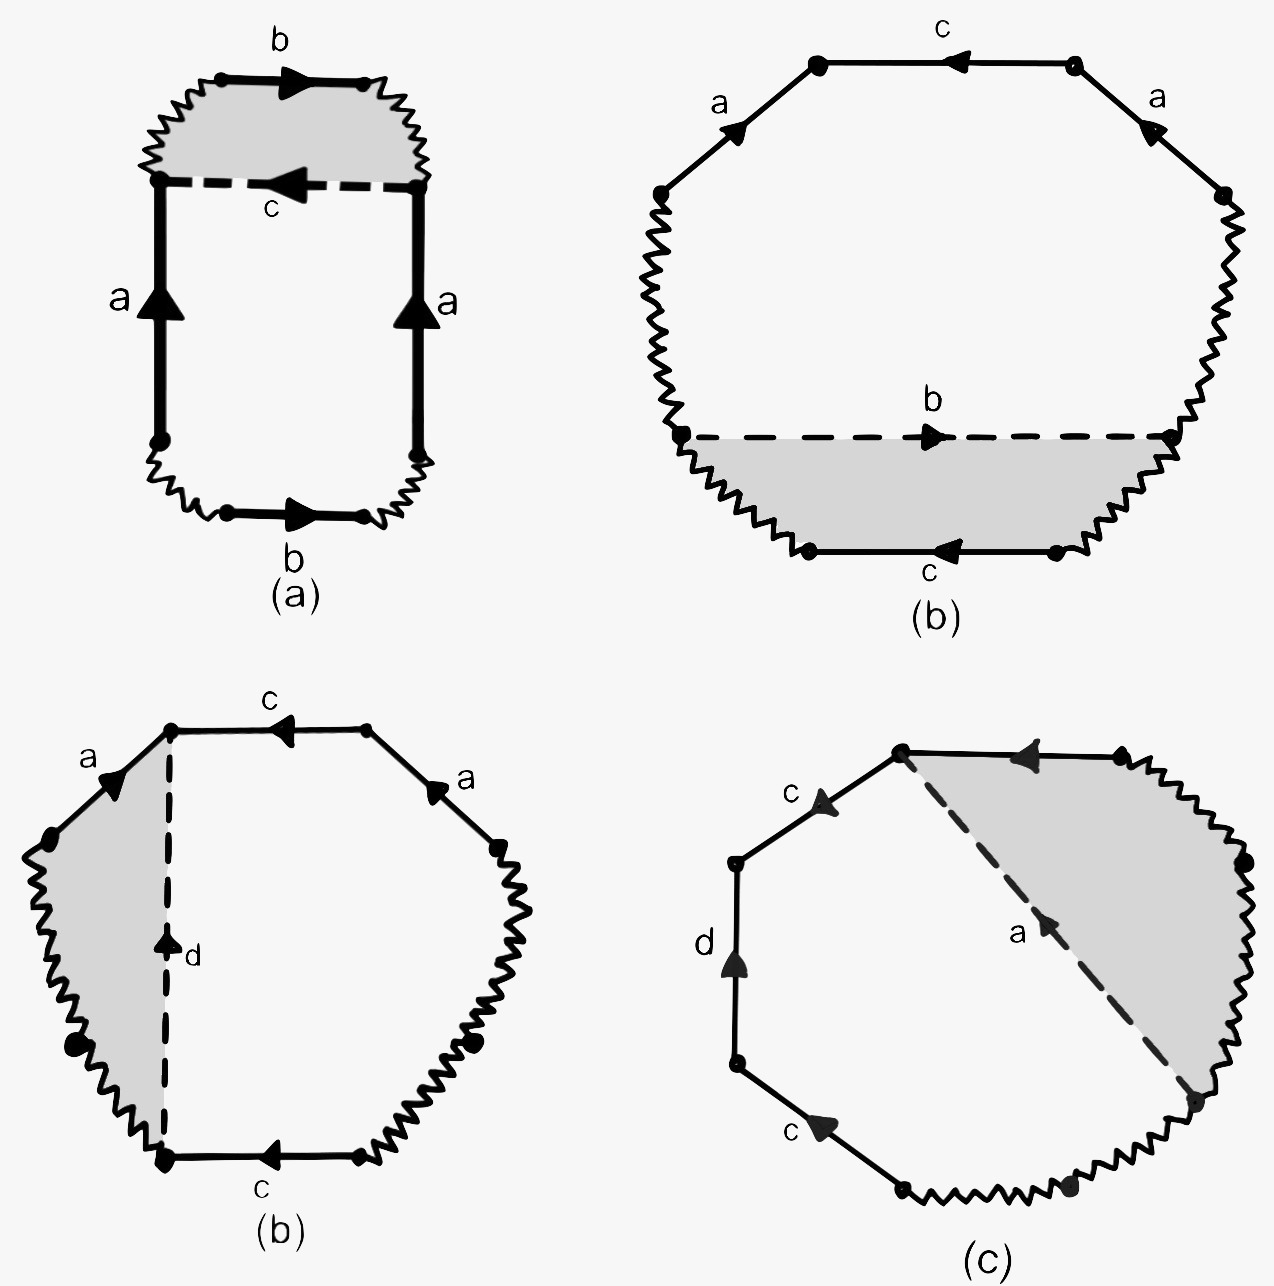
\includegraphics[width=0.4\linewidth]{imagenes/paso5.jpeg}
	\caption{Haciendo adyacentes pares de primera especie intercalados.}
	\label{fig:paso5}
\end{figure}

Repetimos el mismo procedimiento hasta que todos los pares de aristas de primera especie estén agrupados de la forma  $cdc^{-1}d^{-1}$. Si no hay pares de arista de segunda especie, la expresión sería 
\[a_1 b_1 a_1^{-1} b_1^{-1} a_2 b_2 a_2^{-1} b_2^{-1} \ldots a_n b_n a_n^{-1} b_n^{-1}\]
con lo que la superficie es equivalente a una suma conexa de $n$ toros (véase la sección \ref{subsec:expresionescanonicassumasconexas}).


\section{Desenlace final}
\label{sec:desenlacefinal}
Tras los cinco pasos anteriores hemos tenido en cuenta los casos en los que la superficie es homeomorfa a una esfera, una suma conexa de $n$ planos proyectivos o una suma conexa de $m$ toros. Consideremos ahora el caso en el que la expresión tiene tanto aristas de segunda especie (adyacentes), como aristas de primera especie (agrupadas en conjuntos de cuatro). La expresión de este último caso corresponde con una suma conexa de $n$ toros y $m$ planos proyectivos:
\[ a_1 b_1 a_1^{-1} b_1^{-1} \ldots a_n b_n a_n^{-1} b_n^{-1} c_1 c_1 \ldots c_m c_m \] 

Utilizando el lema \ref{lema:planop+toro=3planop}, tenemos que cada suma de toro más plano proyectivo puede sustituirse por la suma conexa de tres planos proyectivos. Del lema se sigue que, en este último caso, nuestra superficie corresponde con una suma conexa de $m+2n$ planos proyectivos, con lo que queda demostrado el teorema.

En virtud de lo mencionado sobre orientabilidad en la sección \ref{sec:orientabilidad}, podemos reformular el teorema de clasificación como:

\begin{teorsin}
Toda superficie compacta orientable es topológicamente equivalente a una esfera o una suma conexa de $n$ toros. Toda superficie compacta no orientable es homeomorfa a una suma conexa de $n$ planos proyectivos.
\end{teorsin}

Definimos entonces el \textit{género} de una superficie compacta como el valor de $n$ que le corresponde por homeomorfismo en el teorema anterior. En caso de que la superficie sea homeomorfa a una esfera diremos que tiene género 0. \\
Para probar que el género está bien definido hace falta demostrar que las clases de equivalencia mencionadas no son homeomorfas entre sí. Una prueba se construye en \cite{massey} utilizando la relación \ref{gen_carE} entre el género ($g$) y la característica de Euler ($x$), y demostrando la invariancia topológica de la característica.
\begin{equation}
\label{gen_carE}
g = \begin{cases}
\frac{1}{2}(2-x) & \quad \text{si la superficie es orientable}\\
2-x & \quad \text{si la superficie no es orientable}
\end{cases}
\end{equation}

\section{Superficies con borde y su clasificación}
\label{sec:superfborde}
La noción de superficie con la que hemos trabajado hasta ahora no contempla `bordes'. Por ejemplo, si tomamos el cuadrado cerrado
\[
\overline{C} = \{(x,y)\in \reales^2:\; 0 \leq x \leq 1, \: 0 \leq y \leq 1  \}
\]
comprobamos que no satisface la definición \ref{defin:superficie}: el punto $(0,0)$ no tiene ningún entorno homeomorfo a $U^2$. Ampliaremos entonces el concepto de superficie:

\begin{defin}
Diremos que un espacio topológico $S$ es una \textit{superficie con borde} si cumple ser conexo, Hausdorff y segundo numerable. Donde, además, se cumple que todo punto en $S$ tiene un entorno homeomorfo a $U^2$ o a
\[H^2 = \{(x,y)\in U^2:\; y\geq0 \}\]
Llamaremos \textit{borde} de la superficie al conjunto de puntos que tienen entornos homeomorfos a $H^2$, e \textit{interior} de la superficie al conjunto de puntos con entornos homeomorfos $U^2$.
\end{defin}

En general, si a una superficie compacta (sin borde) le retiramos el interior de un número finito de discos disjuntos, obtenemos una superficie compacta con borde. El número de componentes del borde es precisamente el número de discos elegidos. 

\begin{figure}[h!]
	\centering
	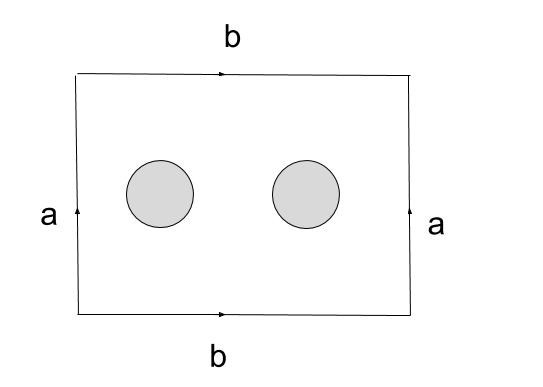
\includegraphics[width=0.3\linewidth]{imagenes/ejemploborde.png}
	\caption{Superficie con borde: Toro con 2 agujeros.}
    \label{fig:superfconborde}
\end{figure}

Podemos formular una especie de recíproco. En una superficie con borde compacta $M$ cuyo borde tiene $k \geq 1$ componentes, se cumple que cada componente es una 1-variedad compacta y conexa, esto es, una circunferencia. A lo largo de cada una de las componentes del borde de $M$ podemos `pegar' un disco cerrado, obteniendo de esa forma una superficie compacta $M^*$ sin borde. Está claro que, si dos superficies compactas con bordes $M_1$ y $M_2$ son homeomorfas, también lo serán las respectivas superficies compactas $M_1^*$ y $M_2^*$. Sin embargo, no resulta tan directo que, si $M_1^*$ y $M_2^*$ son homeomorfas y se han formado de añadir el mismo número de discos cerrados,  entonces también lo serán las superficies con borde compactas iniciales $M_1$ y $M_2$. Enunciamos este resultado en el siguiente teorema:

\begin{teor}
\label{teor:clasifcompactaconborde}
Dos superficies con borde compactas $M_1$ y $M_2$ son homeomorfas si y solo si tienen el mismo número de componentes de borde y las superficies $M_1^*$ y $M_2^*$ son homeomorfas.
\end{teor}

La demostración a este teorema la adjuntamos en el anexo \ref{anexo:teor1}. La prueba utiliza fuertemente la clasificación de superficies compactas sin borde \ref{teor:teoremadeclasificacion} y un razonamiento similar al de su demostración. \\
Utilizando el teorema de clasificación al inicio del capítulo \ref{teor:teoremadeclasificacion}, podemos reformular el resultado anterior \ref{teor:clasifcompactaconborde} como el teorema de clasificación de superficies compactas con borde:

\begin{teorsin}
Toda superficie con $k$ componentes de borde es homeomorfa a una esfera, o a una suma conexa de $n$ toros o a una suma conexa de $n$ planos proyectivos, en los cuales retiramos $k$ discos abiertos.
\end{teorsin}
\noindent \textbf{Obsevación:} este enunciado alternativo nos permite hablar de género también para el caso de las superficies con borde. 

Con esto cerramos finalmente la clasificación para superficies compactas y  podemos sumergirnos en el mundo más variado de la no compacidad.



\chapter{Hacia las superficies no compactas}
En este capítulo extenderemos la clasificación a superficies no compactas y construiremos una superficie representante para cada clase de equivalencia.

El teorema de clasificación de superficies no compactas de Kerékjártó se basará en la clasificación de superficies compactas con borde, estudiada en el capítulo anterior, y en el concepto de `borde ideal', que introduciremos en este capítulo. El borde ideal será un invariante  definido a partir de una superficie dada, que a su vez será un espacio topológico totalmente inconexo, separable y compacto. Finalmente, el teorema nos garantizará que, fijado el género y la `clase de orientabilidad', dos superficies son homeomorfas si y solo si sus bordes ideales también lo son.

Las propiedades topológicas del borde ideal nos permitirán dar representantes para cada clase de equivalencia en la clasificación. Por un lado, veremos que todo borde ideal es homeomorfo a un subconjunto cerrado del conjunto de Cantor. Por el otro, estudiaremos una construcción de Richards que  asigna a todo subconjunto cerrado del conjunto de Cantor una superficie con borde ideal homeomorfo al subconjunto dado. Usando esta construcción una sencilla observación nos permitirá dar con los representantes. Por último, discutiremos brevemente la numerabilidad de las clases de superficies. 

El grueso de nuestra atención en este capítulo irá a la construcción de Richards. Recordamos también que las superficies estudiadas en este trabajo son segundo numerables por definición (\ref{defin:superficie}). 
\section{Introducción a las superficies no compactas}
Las superficies no compactas son objetos que surgen tan pronto uno trabaja con superficies que se ``extienden a infinito''. El plano $\reales^2$ o el grafo de una función suave de $\reales^2$ a $\reales$, son posibles ejemplos de superficies no compactas. La figura \ref{fig:ejemplonocompactas} muestra en las imágenes (a) y (b) dos ejemplos ligeramente más sofisticados  de superficies no compactas que se extienden a infinito. Otra forma de obtener superficies no compactas es retirar discos abiertos o puntos a superficies compactas. Por ejemplo, podemos tomar una esfera y quitarle un punto (imagen (c) de la figura), el resultado obtenido será una superficie no compacta. Un ejemplo más  lo veremos en la figura \ref{fig:nocompactogenero2}, donde tenemos una superficie compacta de género 2 orientable a la que retiramos un punto. Usando este procedimiento podemos construir superficies no compactas variopintas, basta con tomar una superficie compacta de las estudiadas en el capítulo \ref{chap:clasifcompacta} y retirarle un conjunto de puntos. 

\begin{figure}[h!]
	\centering	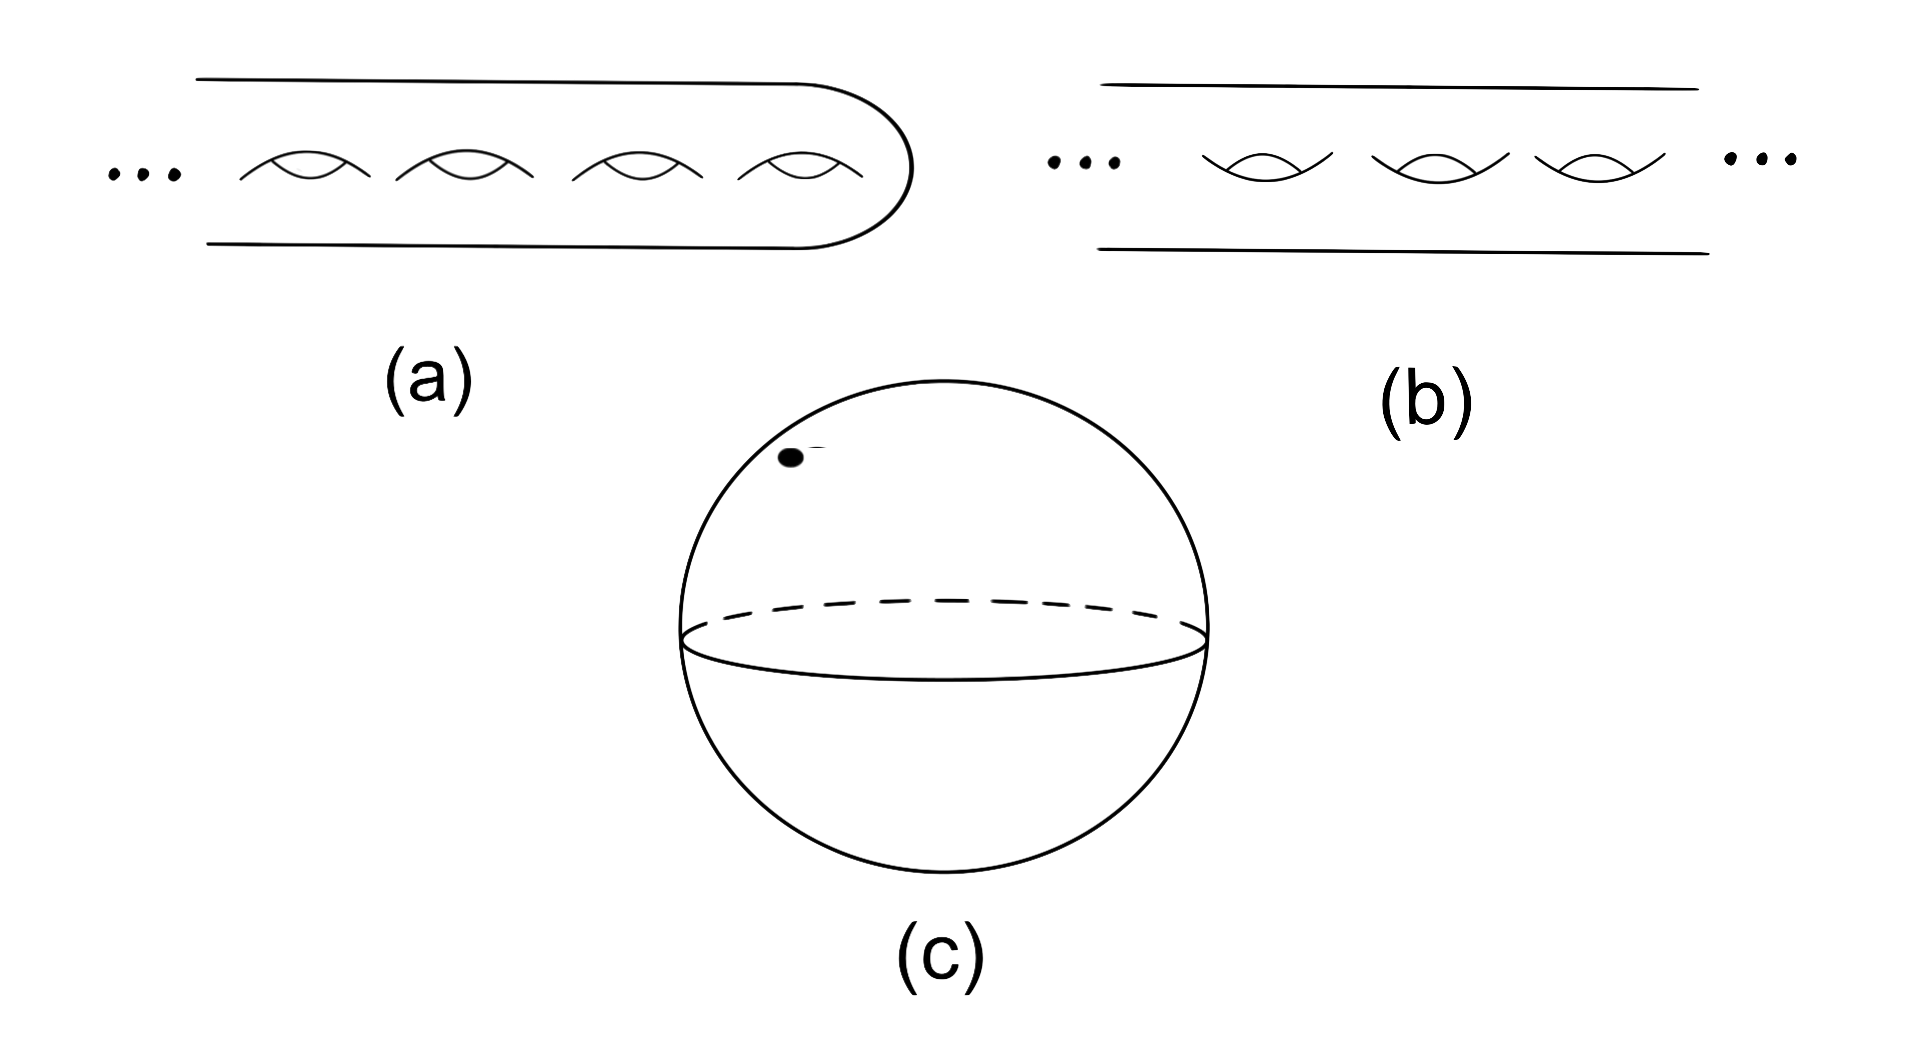
\includegraphics[width=0.5\linewidth]{imagenes/ejemplonocompactas.png}
	\caption{Superficies no compactas.}
	\label{fig:ejemplonocompactas}
\end{figure}

Estudiaremos en este capítulo el concepto de `extremo', que nos permitirá establecer una especie de equivalencia entre `retirar puntos' y `extenderse a infinito' en superficies no compactas. La figura \ref{fig:nocompactogenero2} ofrece una intuición al respecto. 

De los ejemplos que proponemos en la figura \ref{fig:ejemplonocompactas} ya podemos observar las nuevas dificultades que surgen de eliminar la compacidad. Por un lado, todas las superficies mostradas son orientables, sin embargo, (c) es de género 0 mientras que las otras dos tienen `género infinito' (más adelante detallaremos esta noción). Resulta entonces claro, que entre (a) y (c) no habrá homeomorfismo, de haberlo entonces podríamos restringir el homeomorfismo a una subsuperficie de género 1 en (a) pero esta superficie no tendría una correspondiente en (c) del mismo género. Pero no resulta evidente si existe, o no, un homeomorfismo entre (a) y (b), ya que ambas comparten orientabilidad y género. Veremos más adelante que la respuesta es negativa, no existe tal homeomorfimo, y que para formular una clasificación, en el caso no compacto, será necesaria la definición de un nuevo invariante topológico, el borde ideal. El teorema de Kerékjártó \ref{teor:kerekjarto} será el que  garantice que con este nuevo concepto alcanzamos una caracterización completa.

Sin más preámbulos, procedemos a introducir algunas definiciones que serán útiles para el manejo de las superficies no compactas:

Diremos que un subconjunto de una superficie $S$ es \textit{acotado} si su cierre es compacto en $S$. Además, llamaremos \textit{subsuperficie} de  $S$ a cualquier región cerrada cuyo borde en $S$ consista de un número finito de curvas cerradas simples sin autointersecciones. La figura \ref{fig:ejemplonocompacto} ilustra una superficie no compacta con una subsuperficie $S'$, que además cumple ser un subconjunto acotado. 

\begin{figure}[h!]
	\centering	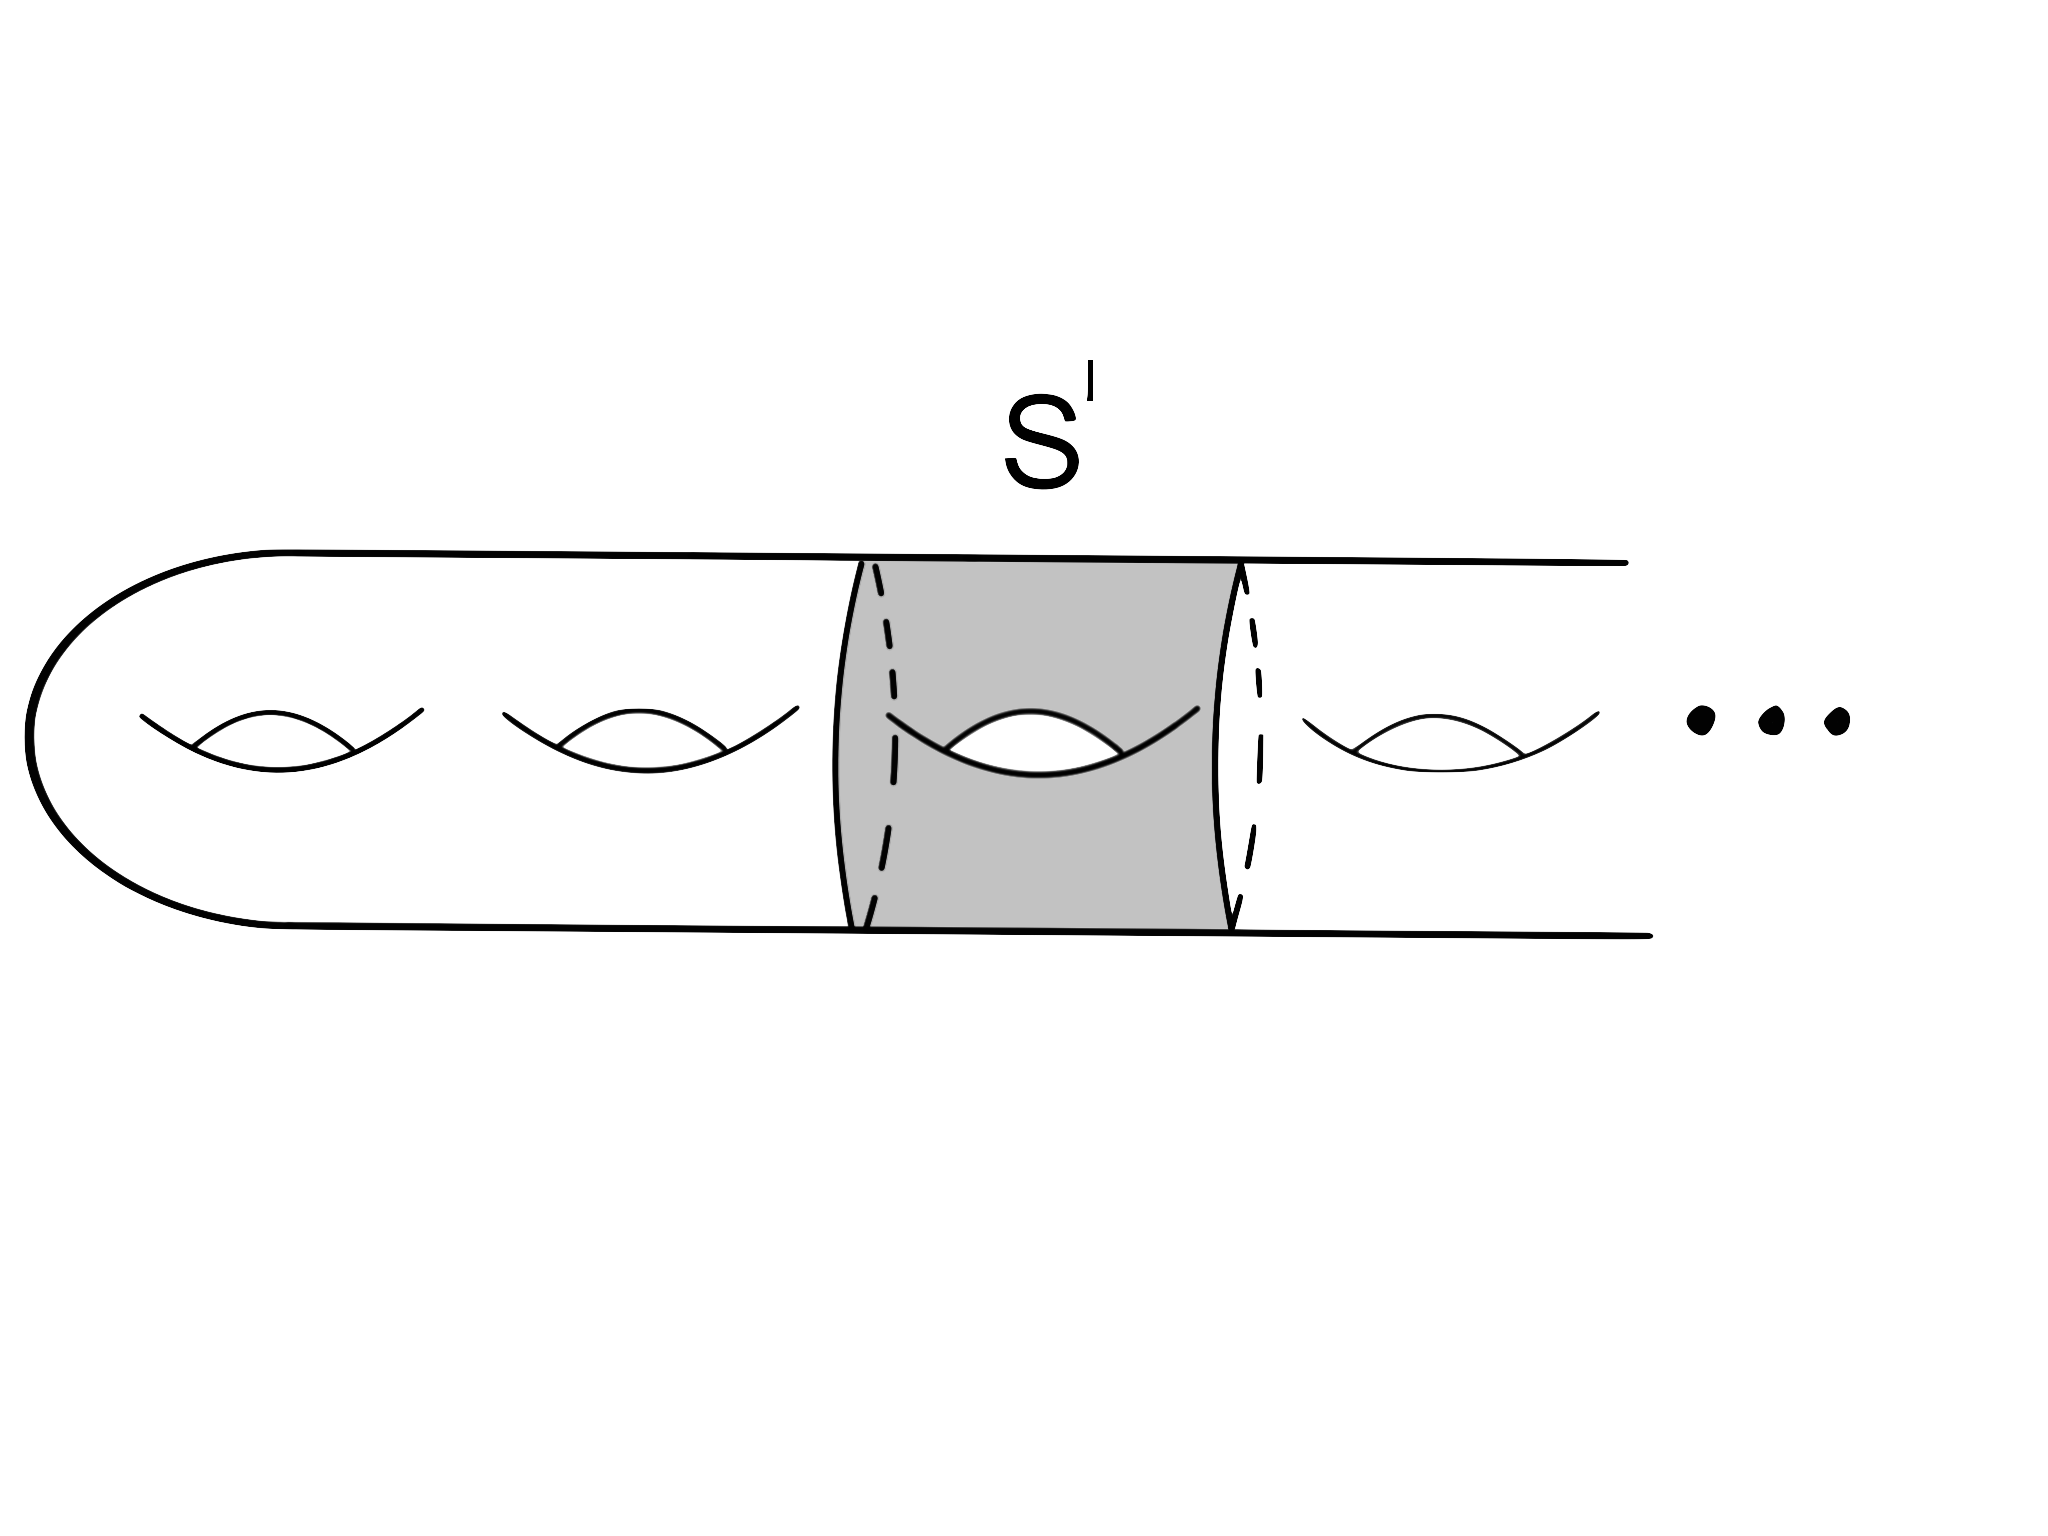
\includegraphics[width=0.5\linewidth]{imagenes/ejemplonocompacta.png}
	\caption{Superficie no compacta con subsuperficie $S'$.}
	\label{fig:ejemplonocompacto}
\end{figure}

\subsection*{Sobre el género}
El género de una superficie no compacta $S$ se define a partir de los géneros de sus subsuperficies compactas:
\begin{defin}
Diremos que una superficie no compacta es \textit{planar} (o de género 0) si toda subsuperficie compacta tiene género 0. 
\end{defin}
Por otra parte, si existe una subsuperficie compacta $A\subset S$ de género $m$, tal que las componentes de $S\backslash A$ son superficies de género 0, entonces diremos que $S$ tiene género $m$. Fijémonos en que esta definición no entra en contradicción con la anterior cuando $m=0$. Si tal superficie $A$ no existiera, entonces diremos que $S$ tiene \textit{género infinito}. En este último caso, se comprueba que existen subsuperficies compactas de género arbitrariamente grande.

Una superficie no compacta de género $m=2$ está representada en la figura \ref{fig:nocompactogenero2}. La imagen (a) corresponde con la suma conexa de dos toros a la que hemos retirado un punto, esta será topológicamente equivalente a la superficie de la imagen (b). Este ejemplo nos da una método para construir superficies no compactas de género finito arbitrario, basta con tomar una superficie de las estudiadas en la sección anterior \ref{chap:clasifcompacta} y retirar un conjunto discreto de puntos o discos abiertos. Por otra parte, la figura \ref{fig:ejemplonocompacto} nos da un ejemplo de una superficie no compacta de género infinito.

\begin{figure}[h!]
	\centering	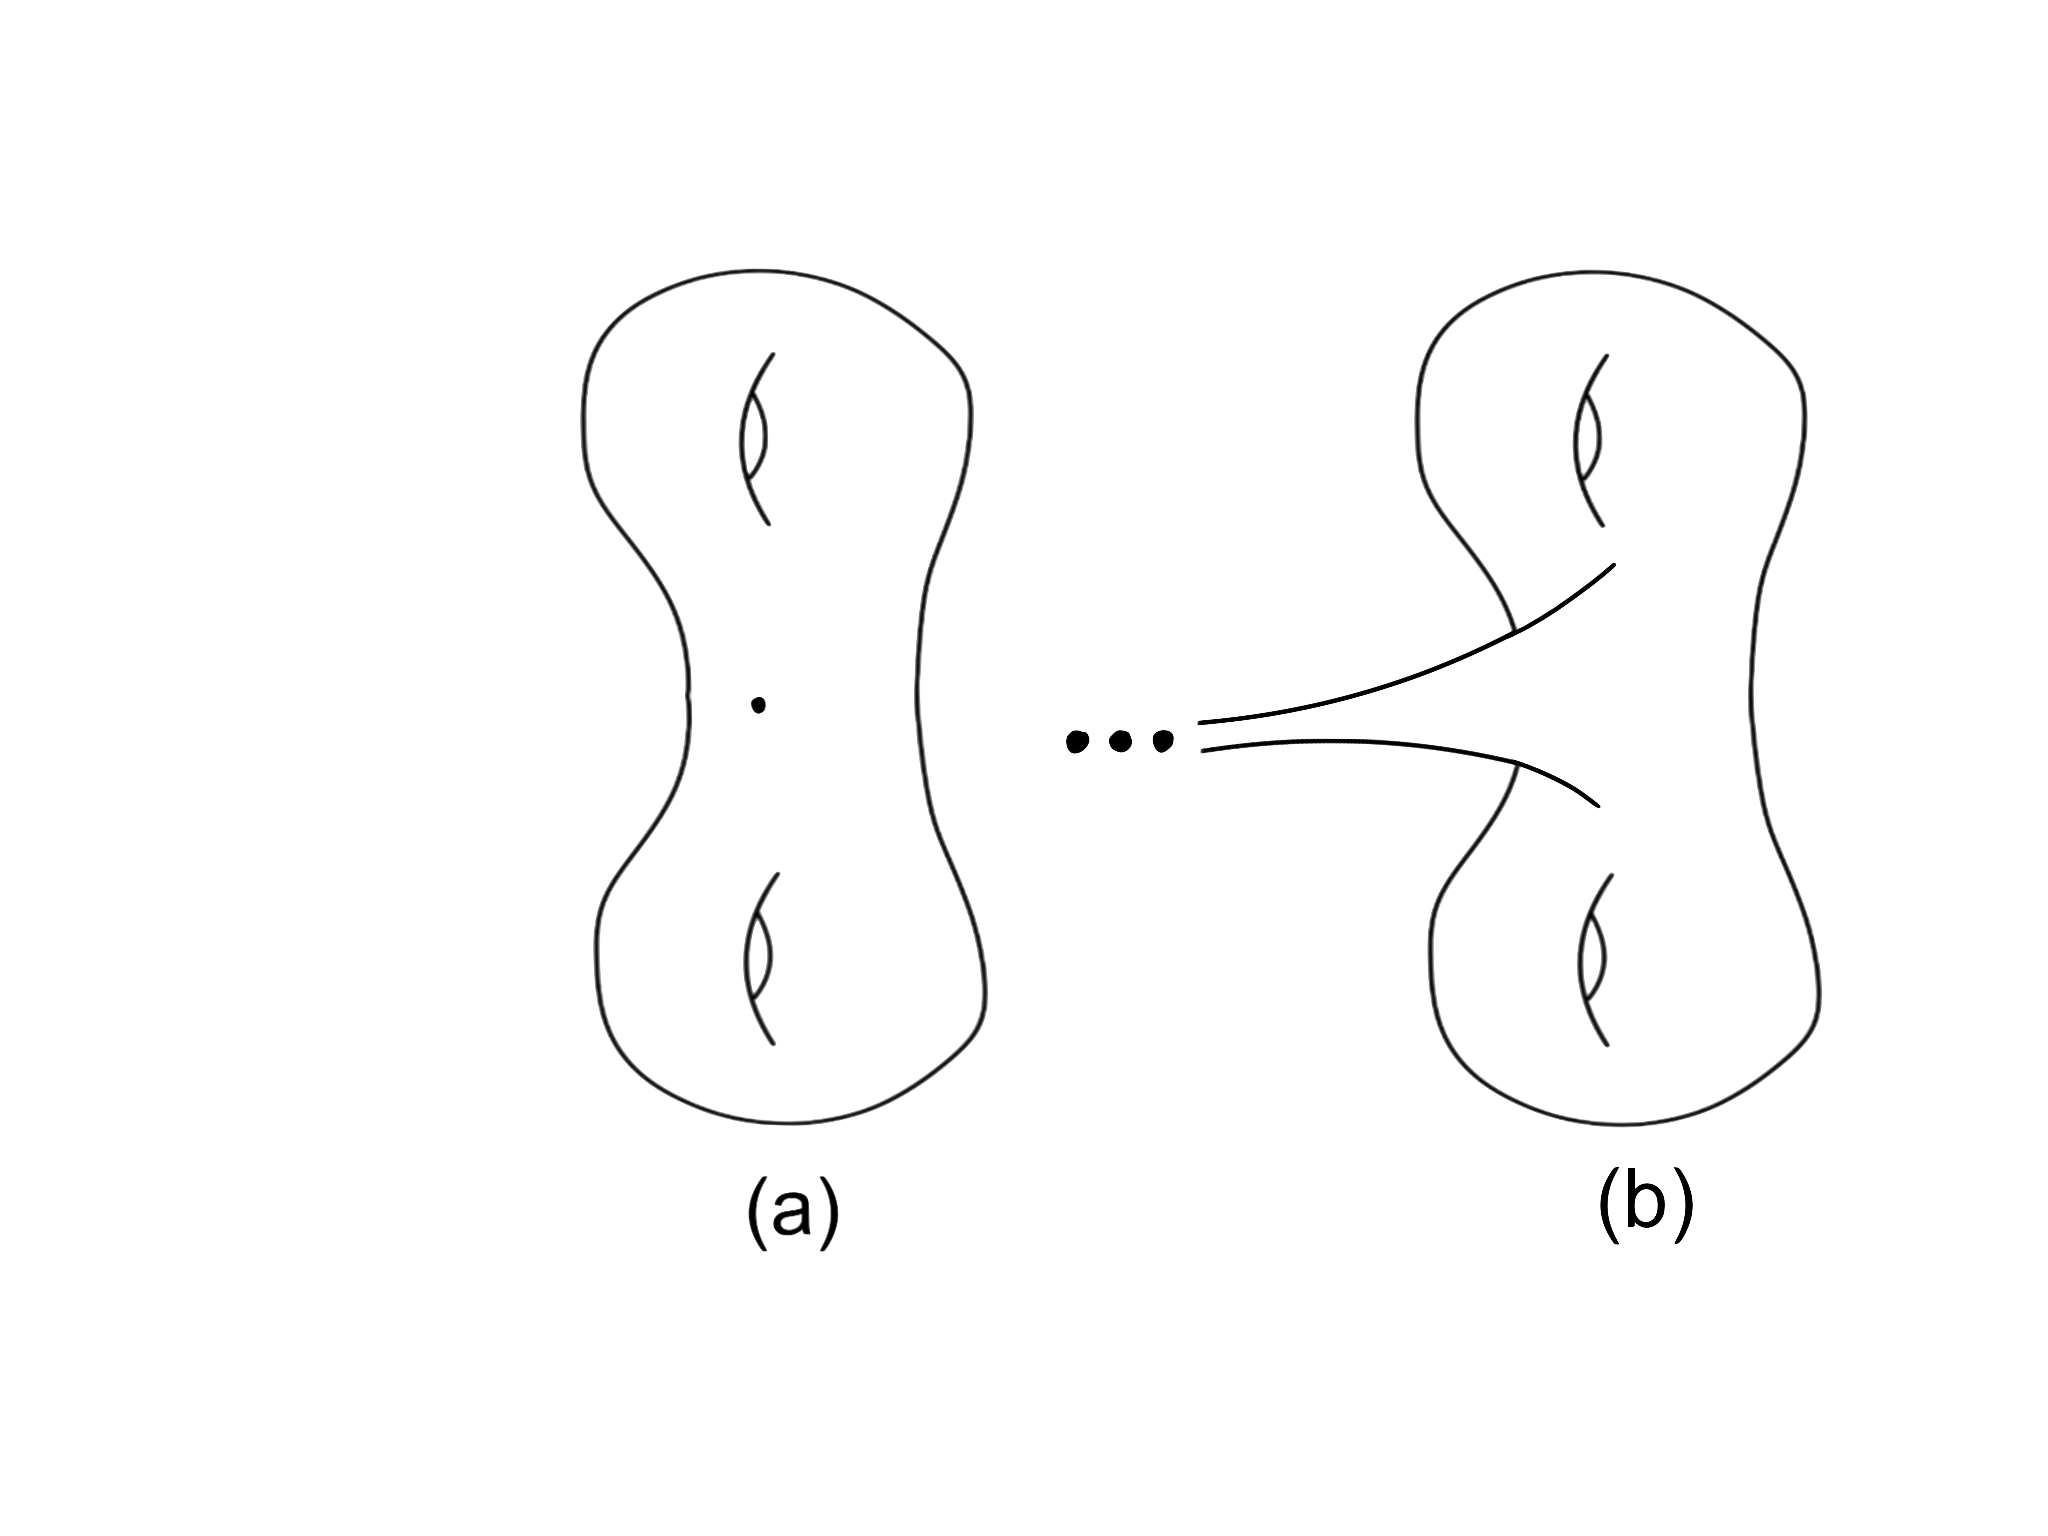
\includegraphics[width=0.5\linewidth]{imagenes/ejemplonocompacta2.png}
	\caption{(a) Suma conexa de dos toros menos un punto.  (b) Superficie no compacta de género 2.}
	\label{fig:nocompactogenero2}
\end{figure}


\subsection*{Sobre la orientabilidad}
De manera similar al caso compacto, las superficies pueden ser orientables o no orientables. Adicionalmente, una superficie $S$  no compacta y no orientable diremos que es \textit{finitamente no orientable} si existe una subsuperficie $A\subset S$ tal que todas las componentes de $S\backslash A$ son orientables. En caso de que $S$ no sea orientable y que no exista un $A$ que cumpla esa propiedad, entonces diremos que la superficie es \textit{infinitamente no orientable}. Observamos que una superficie infinitamente no orientable necesariamente tiene que ser de género infinito (si fuese de género finito tendríamos un $S\backslash A$ con componentes de género 0, y por ende orientable). Sin embargo, el recíproco no es cierto, i.e, hay superficies de género infinito orientables (véase \ref{fig:ejemplonocompacto}).

Una superficie $S$ finitamente no orientable puede ser de \textit{no orientabilidad par o impar} según si una subsuperficie compacta $A$ lo suficientemente grande tiene género par o impar. Esta definición tiene sentido gracias al lema \ref{lema:planop+toro=3planop} que nos asegura que la suma conexa de un toro más un plano proyectivo es homeomorfa a la suma de tres planos proyectivos; lo que nos indica que el número de planos proyectivos no cambia módulo 2 si sumamos una superficie orientable. 
\begin{defin}
Diremos que dos superficies pertenecen a la misma \textit{clase de orientabilidad} si: ambas son orientables; o ambas son infinitamente no orientables; o ambas comparten ser finitamente no orientables de la misma paridad.
\end{defin}


\subsection{El borde ideal}

Más adelante, con el teorema de Kerékjártó \ref{teor:kerekjarto}, comprobaremos que el género y la clase de orientabilidad no son invariantes suficientes para caracterizar una superficie, a diferencia del caso compacto. Por ejemplo, las figuras \ref{fig:ejemplonocompacto} y \ref{fig:extremo} son ambas de género infinito y orientables y, a pesar de ello, no son superficies homeomorfas. Introducimos ahora el `borde ideal' con el que completamos la caracterización.

El borde ideal es un espacio topológico que da una descripción de cómo una superficie se `escapa' a infinito. Se construye como el conjunto de clases de equivalencia de los `extremos', concepto que definimos a continuación:

\begin{defin}
\label{defin:extremo}
Un \textit{extremo} de una superficie $S$ es una secuencia de conjuntos encajados $P_1 \supset P_2 \supset \ldots$, donde $P_i$ es un conjunto conexo no acotado de $S$ que cumple:
\begin{enumerate}
\item[(a)] La frontera de $P_i$ es compacto para todo $i$;
\item[(b)] Para cualquier subconjunto acotado $A \subset S$, $P_i \cap A = \emptyset$ para $i$ suficientemente grande.
\end{enumerate}
\end{defin}
Dados dos extremos $p = P_1 \supset P_2 \supset \ldots$  y  $p' = P'_1 \supset P'_2 \supset \ldots$, diremos que son equivalentes si para todo $n$ existe un correspondiente $N$ tal que $P_n \subset P'_N$ y viceversa.  Esta regla establece una relación de equivalencia. Denotaremos por $p*$ a la clase de equivalencia del extremo $p$.


\begin{figure}[h!]
	\centering
	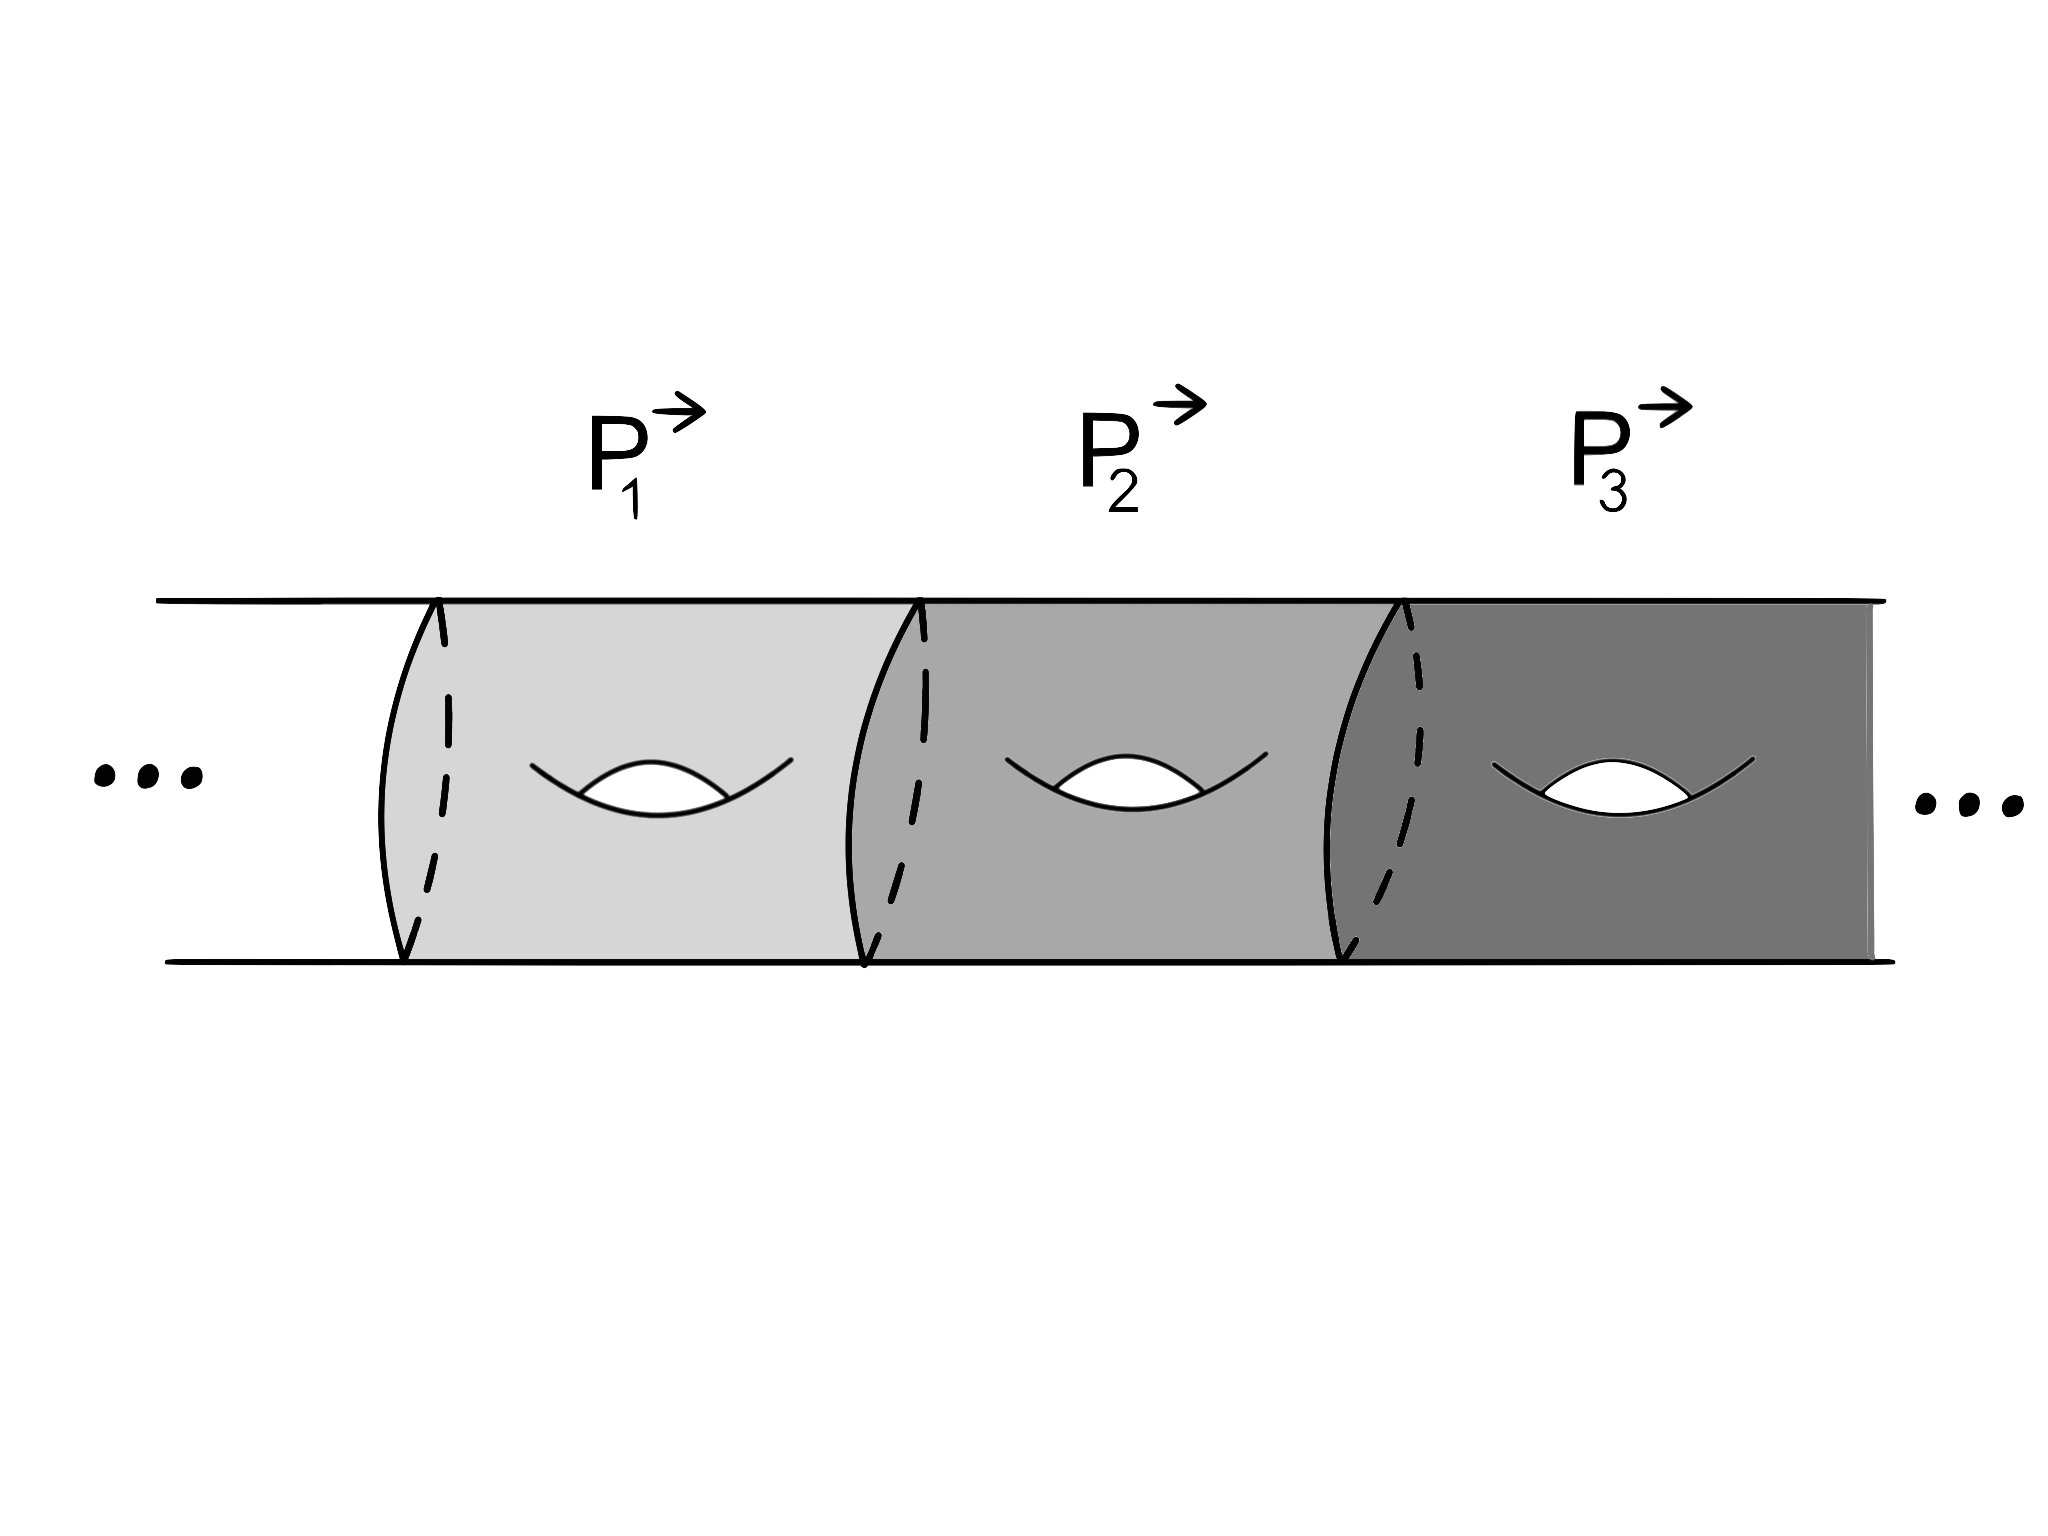
\includegraphics[width=0.5\linewidth]{imagenes/final.png}
	\caption{Ejemplo de un extremo (Los conjuntos $P_i$ se acumulan hacia la derecha).}
	\label{fig:extremo}
\end{figure}

\begin{defin}
El \textit{borde ideal} de una superficie $S$ es el espacio topológico $B(S)$ que tiene por elementos las clases de equivalencia de extremos. La base de la topología está compuesta por los conjuntos $U^*$, donde $U\subset S$ es cualquier conjunto  cuyo borde sea compacto, y los elementos de $U^*$ son los extremos $p*$ que satisfacen que, fijado un representante $p=P_1 \supset P_2 \supset \ldots $, existe un $n$ con $P_n \subset U$.
\end{defin}
Para probar que el borde ideal está bien definido es preciso comprobar que los elementos de cualquier $U^*$ no dependen del representante escogido, esto se sigue directamente de la relación de equivalencia establecida entre extremos. Además, es necesario probar que el conjunto propuesto, en efecto, forma una base de una topología. Para ello comprobamos que: eligiendo $U=\emptyset$ tenemos el abierto $U^*=B(S)$; tomando $U = S$ tenemos el abierto $U^*=\emptyset$; y en el siguiente lema veremos que $U^* \cap V^* = (U \cap V)^*$, lo que prueba que el conjunto es una base y con ello se demuestra que el espacio $B(S)$ está bien definido.

\begin{lema}
\label{lema:intdeextremos}
Dada una superficie $S$ y dos conjuntos  con frontera compacta $U,V \subset S$, entonces se cumple que $U^*\cap V^* = (U \cap V)^* $.
\end{lema}
\begin{proof}
En primer lugar, veamos que $U^*\cap V^* \supset (U \cap V)^* $. Dado un $p^* \in (U \cap V)^*$ y un representante $p = P_1 \supset P_2 \supset \ldots$ de $p^*$, existe un $n$ tal que $P_n \subset (U \cap V)$. Eligiendo el mismo representante y el mismo $n$, tenemos que  $p^* \in U^*$ y $p^* \in V^*$. \\
Por otra parte, veamos $U^*\cap V^* \subset (U \cap V)^* $. Tomando $p^* \in U^* \cap V^*$ y el representante $p = P_1 \supset P_2 \supset \ldots$, entonces existen $n$ y $m$ con $P_n \subset U$ y $P_m \subset V$. Definiendo entonces
 \[ n' = \max(n,m)\]
  comprobamos que $P_{n'} \subset U \cap V$, por lo que $p^* \in (U \cap V)^*$.
\end{proof}

Del mismo modo, conviene demostrar la misma propiedad para la unión:
\begin{lema}
\label{lema:unideextremos}
Dada una superficie $S$ y dos conjuntos  con frontera compacta $U,V \subset S$, entonces se cumple que $U^*\cup V^* = (U \cup V)^* $.
\begin{proof}
Si $U$ y $V$ tienen frontera compacta entonces $U  \cup  V$ también. El contenido $U^*\cup V^* \subset (U \cup V)^* $ se sigue directamente de la definición.\\
El otro contenido lo comprobaremos por contradicción:\\
 Supongamos que $q^* \in (U \cup V)^*$ y que tiene por representante a $q = Q_1 \supset Q_2 \supset \ldots$, pero que para todo $n$ tenemos que $Q_n \nsubseteq U$ y $Q_n \nsubseteq V$. Como la frontera de $U \cup V$ y la de $V^c$ son compactas, podemos elegir un $n$ tal que $\frontera(V^c)\cap Q_n = \emptyset$ y que $Q_n \subset \interior(U\cup V)$. Entonces proponemos  la partición de $Q_n$ en los abiertos $\interior(V) \cap \interior(U \cup V)$ e  $\interior(V^c) \cap \interior(U \cup V)$, disjuntos y ambos con intersección con $Q_n$ no vacía por la hipótesis inicial; sin embargo, esto contradice que $Q_n$ sea conexo.
\end{proof}
\end{lema}

\begin{defin}
Sea $p^*$ el representante de un extremo $p =P_1 \supset P_2 \supset \ldots$, diremos que $p^*$ es \textit{plano/orientable} si existe un $N$ tal que para todo $n>N$ los conjuntos $P_n$ son superficies planas/orientables.
\end{defin}
En la figura \ref{fig:m4} ilustramos una superficie con diferentes tipos de extremos: planos, de género infinito orientables y de género infinito no orientables. Otro ejemplo de extremo plano lo observamos en cualquier superficie compacta a la que retiremos un punto (como en la imagen (a) de la figura \ref{fig:nocompactogenero2}), de hecho, por cada punto eliminado estaremos añadiendo un nuevo extremo plano.

La definición anterior nos permite considerar los conjuntos $B(S) \supset B'(S) \supset B''(S)$, donde $B'(S)$  es el conjunto de los extremos no planos y $B''(S)$ es el conjunto de los extremos no orientables. A partir de ahora consideraremos el borde ideal como la terna $(B(S), B'(S), B''(S))$.
\begin{lema}
Los conjuntos $B'(S)$ y $B''(S)$ son cerrados de $B(S)$. 
\end{lema}
\begin{proof}
Veamos que $A = (B'(S))^c$ es un abierto:\\
Sea $p^* \in A$ y $p = P_1 \supset P_2 \supset \ldots$ un extremo representante de la clase $p^*$, entonces existe un $n$ con $P_n$ plano. Definimos el conjunto:
\[
C = \bigcup_{p^* \in A} \interior(P_n)^*
\]
$C$ es abierto por ser unión de abiertos. Bastaría con ver que $C=A$: por un lado, se sigue de la definición que $A\subset C$; por otro, si $q^* \in C$ entonces existe un $n$ y un $m$ con $Q_m \subset \interior(P_n)$, como $P_n$ es plano entonces $Q_m$ también, con lo que concluimos que $q^* \in A \Rightarrow C\subset A$.\\
Una demostración totalmente análoga comprueba que $B = (B''(S))^c$ es abierto.
\end{proof}
\noindent \textbf{Ejemplo:} Si para todo subconjunto compacto $A\subset S$, se tiene que $S\backslash A$ tiene como mucho $m$ componentes no acotadas, y se cumple que para algún $A$ el valor es exactamente $m$, entonces el conjunto $B(S)$ consiste en $m$ clases de equivalencia de extremos (donde cada uno puede ser plano, orientable y no plano, o no orientable). Si $m=0$ tenemos una superficie compacta. La figura \ref{fig:m4} ilustra el caso de $m=4$.


\begin{figure}[h!]
	\centering
	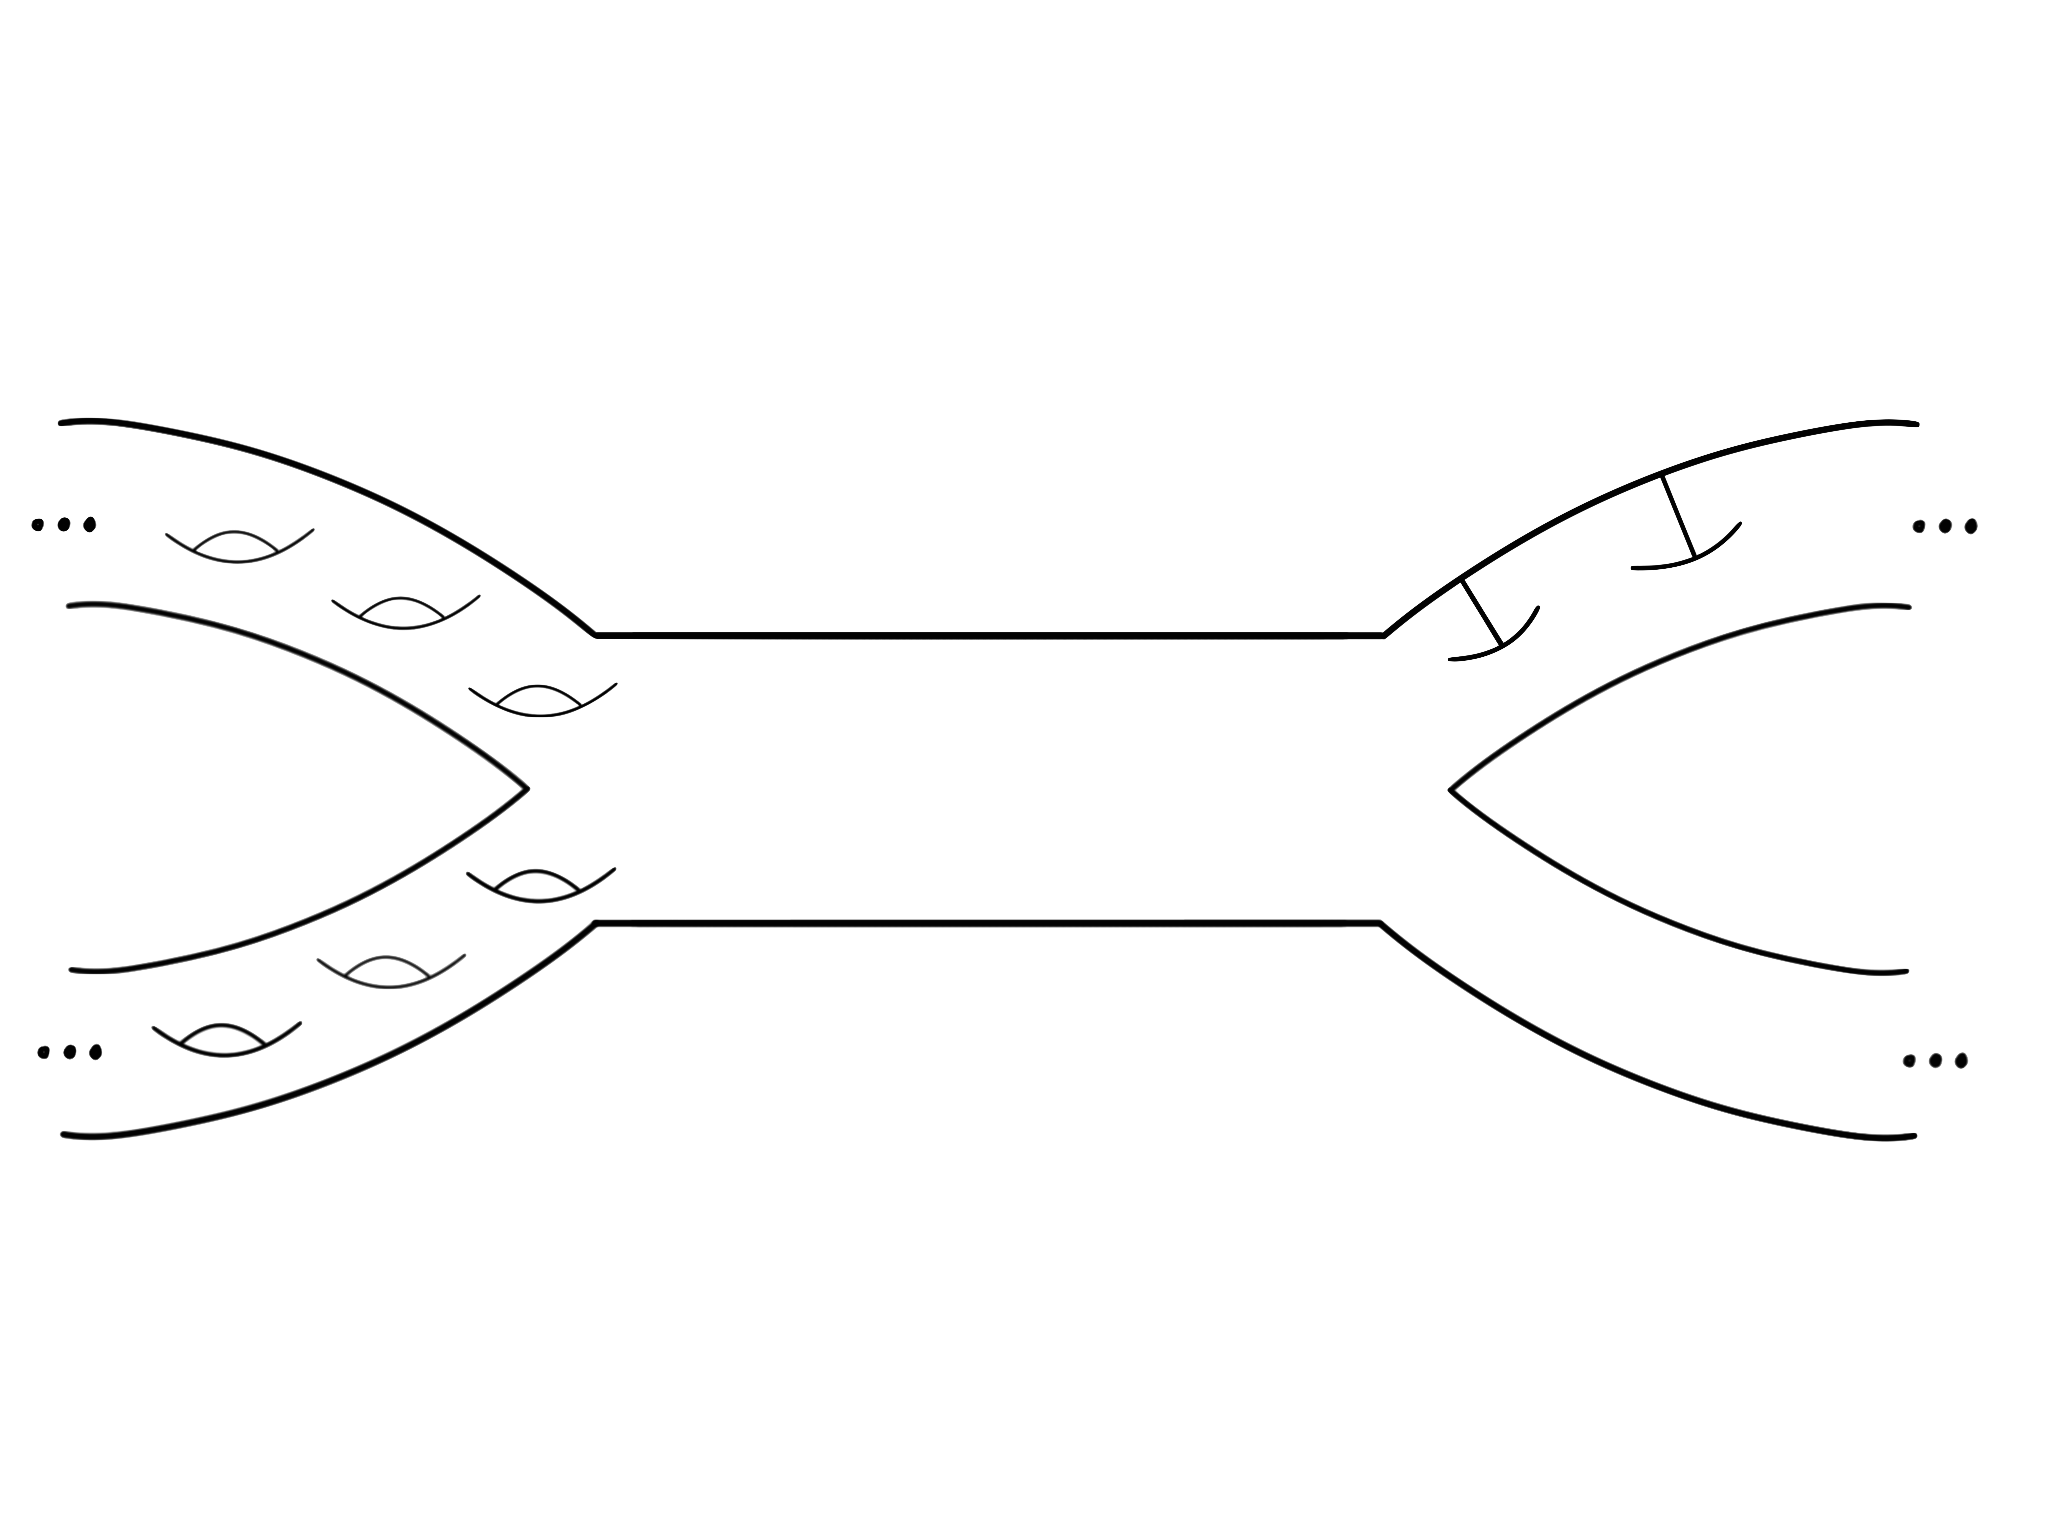
\includegraphics[width=0.5\linewidth]{imagenes/m4.png}
	\caption{Ejemplo con $m=4$: dos extremos de género infinito orientables, uno de género infinito no orientable y un extremo plano.}
	\label{fig:m4}
\end{figure}

Es conveniente tener en cuenta las siguientes propiedades del borde ideal:

\begin{lema}
\label{lema:bordeidealcantor}
El borde ideal de una superficie separable es un espacio $T_2$, totalmente inconexo, separable y compacto. 
\end{lema}
Una demostración rigurosa de este lema se puede conseguir en \cite{Ahlfors}. La siguiente propiedad será interesante más adelante en la construcción de Richards.

\begin{lema}
\label{lema:bordeidealcantor2}
Todo espacio topológico $X$ totalmente inconexo, separable y compacto, es homeomorfo a un subconjunto cerrado del conjunto de Cantor. En particular, el borde ideal de una superficie satisface esta condición.
\end{lema}

En líneas generales, la prueba construye una base numerable de abiertos-cerrados y, sirviéndose de la función característica, construye una función $\phi$ al espacio $\{0,1\}^\mathbb{N}$. Se puede demostrar que esta función $\phi$ es un homeomorfismo a su imagen y, como el espacio $\{0,1\}^\mathbb{N}$ es topológicamente equivalente al conjunto de Cantor, tenemos que nuestro espacio topológico lo será a un subconjunto del conjunto de Cantor.

\section{Teorema de Kerékjárto}
\begin{teor}
\label{teor:kerekjarto}
Sean $S$ y $S'$ dos superficies separables del mismo género y clase de orientabilidad. Entonces $S$ y $S'$ son homeomorfas si y solo si los bordes ideales son homeomorfos como ternas de espacios.
\end{teor}
\noindent \textbf{Nota:} Los bordes ideales $(B(S), B'(S), B''(S))$ y $(B(S'), B'(S'), B''(S'))$ son homeomorfos como ternas de espacios si existe el homeomorfismo $f: B(S) \rightarrow B(S')$, que satisface también que $f(B'(S)) = B'(S') $ y $f(B''(S)) = B''(S')$. En general, cuando hablemos de homeomorfismo entre bordes ideales haremos siempre referencia al homeomorfismo como ternas de espacios.

\begin{proof}[Idea de la demostración]
La demostración sigue un razonamiento inductivo, para demostrarlo son necesarios varios pasos técnicos. En este trabajo esbozaremos sólo la idea que hay detrás de la demostración.

El primer paso consiste en descomponer las superficies $S$ y $S'$ como sucesiones subsuperfecies compactas encajadas. Tomamos dos sucesiones de subsuperficies compactas $B_1 \subset B_2 \subset \ldots$ y $B'_1 \subset B'_2 \subset \ldots$, de modo que recubran a $S$ y $S'$, respectivamente. Además, a cada $B_i$ le exigimos  que separe las componentes de su complementario por una única curva, i.e, por cada componente $U$ de $S\backslash B_i$  pedimos que $U$  tenga una única curva simple cerrada en su frontera $d(U)$ (la misma condición se debe satisfacer para la sucesión con las primas).

A partir de aquí, la demostración buscará construir inductivamente otras dos sucesiones de subsuperficies compactas y una sucesión de funciones $\{f_n\}_{n=1}^{\infty}$ entre estas subsuperficies. Las sucesiones $A_1 \subset A_2 \subset \ldots$ y $A'_1 \subset A'_2 \subset \ldots$, recubrirán a $S$ y $S'$, respectivamente. Por su parte, cada función $f_{n+1}$ establecerá un homeomorfismo entre las superficies con borde   $A_{n+1}$ y $A'_{n+1}$, cumpliendo ser una extensión de $f_n$. Para el argumento inductivo que prueba existencia de las ternas $(A_n, A'_n, f_n)$ se utiliza el homeomorfismo entre los bordes ideales. A partir de allí, el homeomorfismo entre las superficies $S$ y $S'$ será el límite de la sucesión $\{f_n\}$.

\end{proof}


\section{Construcción de una superficie con borde ideal dado}
En esta sección estudiaremos en detalle la construcción de Richards. Recordemos que la proposición \ref{lema:bordeidealcantor} nos garantiza que el borde ideal es un espacio totalmente inconexo, separable y compacto. Demostraremos ahora que para cualquier terna de espacios topológicos $X \supset Y \supset Z$, con $Y$ y $Z$ cerrados de $X$, y con $X$ totalmente inconexo, separable y compacto, existe una superficie con borde ideal homeomorfo a esa terna.\\

\begin{teor}
\label{teor:richards}
Sea $(X,Y,Z)$ una terna cualquiera de espacios compactos, separables y totalmente inconexos con $Z \subset Y \subset X$, donde $Z$ e $Y$ son cerrados de $X$.  Entonces existe una superficie $S$ cuyo borde ideal $(B(S), B'(S), B''(S))$  es homeomorfo a $(X,Y,Z)$
\end{teor}

La construcción partirá de una esfera a la cual retiraremos un conjunto de puntos y discos abiertos, cada punto representará un extremo y los discos serán convenientemente identificados para crear  subsuperficies de género 1 (o bien un toro o bien un plano proyectivo). Configurando adecuadamente estos dos elementos, conseguiremos un borde ideal homeomorfo a $(X,Y,Z)$. Procederemos primero construyendo la superficie, y luego comprobando que cumple la condición especificada.


\begin{proof}[Demostración del teorema \ref{teor:richards}]

Por el lema \ref{lema:bordeidealcantor2} podemos asumir que $X$ es un subconjunto cerrado del conjunto de Cantor, el cual consideramos inmerso en el plano compactificado (homeomorfo a la esfera) como el conjunto de puntos $(x,0)$ con $0 \leq x\leq 1$, donde $x$ tiene una expresión triádica sin el dígito 1.


Elegimos $D'$ el conjunto de todos los discos cerrados del plano que tienen por diámetro los intervalos $[\frac{n - 1/3}{3^m} , \frac{n + 4/3}{3^m} ] \times \{0\}$ , con $0\leq n \leq 3^m$, donde $m$ es cualquier natural y $n$ es un natural que admite una expresión triádica sin el dígito 1. Sea $D$ el subconjunto de discos de $D'$ que contienen al menos un punto de $X$.\\


\begin{figure}[h!]
	\centering
	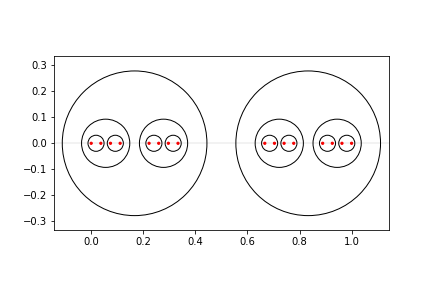
\includegraphics[width=0.5\linewidth]{imagenes/conjuntoD.png}
	\caption{Discos de $D'$, en rojo puntos del conjunto de Cantor.}
	\label{fig:conjuntoD}
\end{figure}

Los discos de $D$ intersecados con $X$ determinan una base de la topología de $X$. Además, cumplen las siguientes dos propiedades:
\begin{enumerate}
\item Cualesquiera dos discos del conjunto son o bien disjuntos o bien uno está contenido dentro del otro (véase la figura \ref{fig:conjuntoD}).
\item Si tenemos una cadena de discos encajados $D_1 \supset D_2 \supset \ldots$, entonces la intersección de todos esos discos  con el eje x es un único punto de $X$ (este hecho se comprueba ya que $X$ es cerrado y, por tanto, compacto). Más aún, se tiene que el conjunto de discos de $D$ que contienen a un $x \in X$ se puede representar como una secuencia $D_1 \supset D_2 \supset \ldots$ cuya intersección es $x$.
\end{enumerate}
Sea $P^+$ y $P^-$ los planos $y > 0 $ e $y < 0$, respectivamente. Para cada disco $K$ en $D$, denotamos por $K'$ y por $K''$ los dos discos más grandes contenidos propiamente en $K$ (cualquier otro disco propiamente contenido en $K$ estará por tanto contenido o en $K'$ o en $K''$, véase la figura \ref{fig:conjuntoD}).

Ahora, para cada disco $K$ en $D$ elegimos dos discos abiertos $C^+(K)$ y $C^-(K)$, cada uno contenido en $K$  y que satisfacen:
\begin{enumerate}
\item[(a)] $C^+(K) \subset P^+$ y $C^-(K) \subset P^-$
\item[(b)] $C^+(K)$ y $C^-(K)$ no intersecan ni a $K'$ ni a $K''$.
\item[(c)] $C^+(K)$ y $C^-(K)$ son simétricos respecto al eje x.
\end{enumerate}
En particular, los círculos $C^\pm(K)$ no se intersecan entre sí.

\begin{figure}[h!]
	\centering
	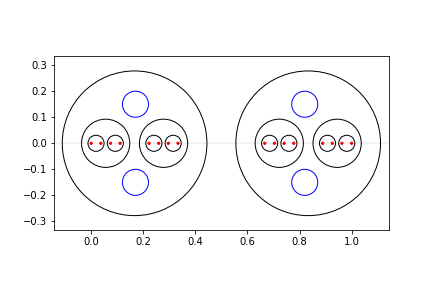
\includegraphics[width=0.5\linewidth]{imagenes/eleccionCK.png}
	\caption{En azul mostramos posibles elecciones de $C^\pm(K)$ .}
	\label{fig:eleccionCK}
\end{figure}

Vamos a construir nuestra superficie $S$ como la esfera homeomorfa al plano compactificado en el que retiramos los puntos de $X$ y algunos de los círculos $C^\pm(K)$. De manera más concreta, retiramos los círculos $C^\pm(K)$ que están dentro de un $K\in D$ con $K \cap Y \neq \emptyset$. Si por el contrario  $K \cap Y = \emptyset$, entonces no retiramos los círculos. Este caso se corresponderá con los extremos planos. A continuación,  si ocurre que $K \cap Y \neq \emptyset$  y $K \cap Z = \emptyset$, entonces identificamos la frontera de $C^+(K)$ con la frontera de $C^-(K)$ reflejando la primera en el eje x (preservando la orientación). Estos casos se corresponderán con los extremos de género infinito orientables.  Por último, si $K \cap Z \neq \emptyset$, entonces identificamos los círculos por traslación (invirtiendo la orientación), en cuyo caso tendremos extremos de género infinito no orientables.

Es fácil comprobar que el conjunto cociente $S$ construido es una superficie, queda ahora probar su borde ideal es homeomorfo a la terna $(X,Y,Z)$:\\
De los puntos (1) y (2) anteriores se sigue que todo punto $x\in X$ se puede representar como la intersección de una secuencia de discos $D_1 \supset D_2 \supset \ldots$, con $D_i \in D$. Utilizando la definición \ref{defin:extremo}, observamos que dichas secuencias de discos son extremos. Esto nos permite definir la función que manda cada $x$ a la correspondiente clase de extremos:
\begin{align*}
f:& \: X \longrightarrow  B(S)\\
& \: x \longrightarrow f(x) = p^*
\end{align*}
donde $p^*$ es representante de $p = D_1 \supset D_2 \supset \ldots $ y se cumple:
\[
\{x\} = \bigcap_{i = 1}^{\infty} D_i
\]
Veamos ahora que $f$ define el homeomorfismo que buscamos.

Como $X\backslash Y$ y $X\backslash Z$ son subconjuntos abiertos de $X$, entonces para todo punto $p\in X\backslash Y$ existe un disco $K\in D$ que contiene a $p$ y cumple $K \cap Y = \emptyset$. Se prueba de forma análoga para $p \in X\backslash Z$. Por tanto, tendremos que $Y$ y $Z$ corresponden exactamente con los extremos no planos y los no orientables, respectivamente (Esto se sigue de que $X\backslash Y$ corresponde por construcción con los extremos planos, y $X\backslash Z$ corresponde con los orientables). Esto indica que $f$ induce los homeomorfismos adecuados cuando se restringe a los espacios $Y$ y $Z$.

La función $f$ es inyectiva porque dados  dos puntos distintos  $x_1, x_2 \in X$ tenemos que, por ser $X$ un espacio Hausdorff, existen dos abiertos $U_1, U_2$ con intersección nula que los separan. Al mismo tiempo, por ser $D$ una base de la topología de $X$, existen dos discos en $D$ que cumplen $x_1 \in K_1 \subset U_1$ y $x_2 \in K_2 \subset U_2$, pero como ambos discos tienen intersección vacía se sigue de la definición \ref{defin:extremo} que las secuencias necesariamente representan extremos no equivalentes.

Por otra parte, vemos que $f$ manda la base inducida por $D$ (intersecando los discos con $X$) de la topología de $X$ al conjunto $\{K^*: K\in D\}$. Utilizando los lemas \ref{lema:unideextremos} y \ref{lema:intdeextremos}, podemos comprobar que dicho conjunto es una base de la topología de $B(S)$. Bastaría entonces con probar la sobreyectividad de $f$ para demostrar que la función es, en efecto, un homeomorfismo.

Probemos que $f$ es sobreyectiva: Como $B(S)$ es Hausdorff, entonces todo punto $p^* \in B(S)$ es intersección de una colección infinita $\{K_i^*\}_{i\in\mathbb{N}}$ de conjuntos de la base $\{K^*: K\in D\}$ de la topología de $B(S)$. Por la condición (1), la colección $\{K_i\}_{i\in\mathbb{N}}$ es una secuencia encajada y representa un extremo $p_1^* \in B(S)$, pero entonces es necesario que $p_1^* = p^*$.  Por la condición (2), se cumple que $\bigcap_{i\in\mathbb{N}} K_i = {p'}$. Finalmente, por la construcción dada de $f$ tenemos que $f(p') = p_1^* = p^*$, probando así la sobreyectividad y con ello concluyendo el teorema.

\end{proof}

\subsection{Construcción de representantes para superficies no compactas}
\label{sec:representantesnocompactos}
Por el teorema de Kerékjártó \ref{teor:kerekjarto}, podemos tomar las superficies construidas en la demostración anterior como representantes para el caso de superficies planas, para superficies de género infinito orientables y para superficies de género infinito e infinitamente no orientables, ya que en estos casos las propiedades de género y clase de orientabilidad vienen determinadas por su borde ideal. Faltaría por asignar un `modelo' a las superficies de género finito y las superficies de género infinito pero finitamente no orientables.

En el caso de una superficie $S$ de género finito $m>0$, podemos asignar el representante $S_1\# S_2$, donde $S_1$ tiene borde ideal homeomorfo al de $S$ y se construye siguiendo la demostración anterior, y $S_2$ es una superficie compacta que es o bien suma conexa de $m$ toros (caso orientable) o bien suma conexa de $m$ planos proyectivos (caso no orientable). Se sigue de las definiciones de borde ideal que sumar una superficie compacta no va a modificar el espacio topológico $B(S)$.

De manera similar, si la superficie $S$ es de género infinito pero finitamente no orientable, el representante se construye igual que el caso anterior ($S_1\# S_2$), pero eligiendo $S_2$ como suma conexa de 2 o 3 planos proyectivos según la paridad de la no orientabilidad.

Comprendidos estos casos, ya tenemos una clasificación completa de las superficies no compactas.

\subsubsection*{Numerabilidad de las clasificaciones}
Las clasificaciones dadas en las secciones anteriores nos permiten acabar el trabajo discutiendo brevemente sobre la cardinalidad de los conjuntos de superficies. 

\begin{teor}
Salvo homeomorfismo, existen $\aleph_0$ superficies compactas y $2^{\aleph_0}$ superficies no compactas.
\end{teor}
El primer resultado se sigue del teorema de clasificación para superficies compactas \ref{teor:teoremadeclasificacion}, completándolo con que las clases propuestas no son homeomorfas entre sí (véase el final de la sección \ref{sec:desenlacefinal}). Por su parte, el segundo resultado se prueba contando los represnetantes discutidos en la sección anterior \ref{sec:representantesnocompactos}, y teniendo en cuenta que existen $2^{\aleph_0}$ subconjuntos cerrados del conjunto de Cantor no homeomorfos \cite{cerradoscantor}. Por último, mencionamos que, si  en la definición de superficie no se exige la condición de segundo numerabilidad, entonces tenemos que la cardinalidad asciende a $2^{\aleph_1}$ \cite{nosegundonomuerable}. Recordemos que esta condición fue siempre instrumento clave en nuestro trabajo, ya que nos permite suponer la existencia de una triangulación.




\chapter{Anexo}
Adjuntamos aquí las demostraciones de algunos resultados para facilitar la lectura del resto del trabajo.

\section{Tres planos proyectivos son topológicamente equivalentes a un toro más un plano proyectivo}
\label{anexo:lema1}
\begin{proof}[Demostración del lema \ref{lema:planop+toro=3planop}]


Ya vimos en  el lema \ref{lema:SumaDosPlanospEsKlein} que la suma conexa de dos planos proyectivos es topológicamente equivalente a una botella de Klein. Además, en la demostración del mismo lema, vimos que un plano proyectivo sin un disco cerrado es topológicamente equivalente a una banda de M\"obius. Concatenando estos dos resultados, tendremos que para probar nuestro lema bastará con demostrar que la suma conexa de un toro con una banda de M\"obius es homeomorfa a la suma conexa de una botella de Klein con una banda de M\"obius. Probaremos entonces este último hecho. A partir de ahora nos referiremos a la banda de M\"obius como la superficie $S$ para facilitar la notación.

Para la demostración será conveniente expresar la suma conexa de forma distinta a lo visto en la sección \ref{sec:sumaconexa}. Iniciamos, representando el toro y la botella de Klein como rectángulos con los lados opuestos identificados como muestra la figura \ref{recorte1}. Posteriormente, la suma conexa la formaremos recortando el disco indicado en los diagramas  con su análogo en $S$, y procedemos a hacer la identificación en dos pasos: primero, pegamos la parte del toro (o botella de Klein) que es imagen del rectángulo $ABB'A'$, y después pegamos el resto del toro (o botella de Klein). 

\begin{figure}[h!]
	\centering
	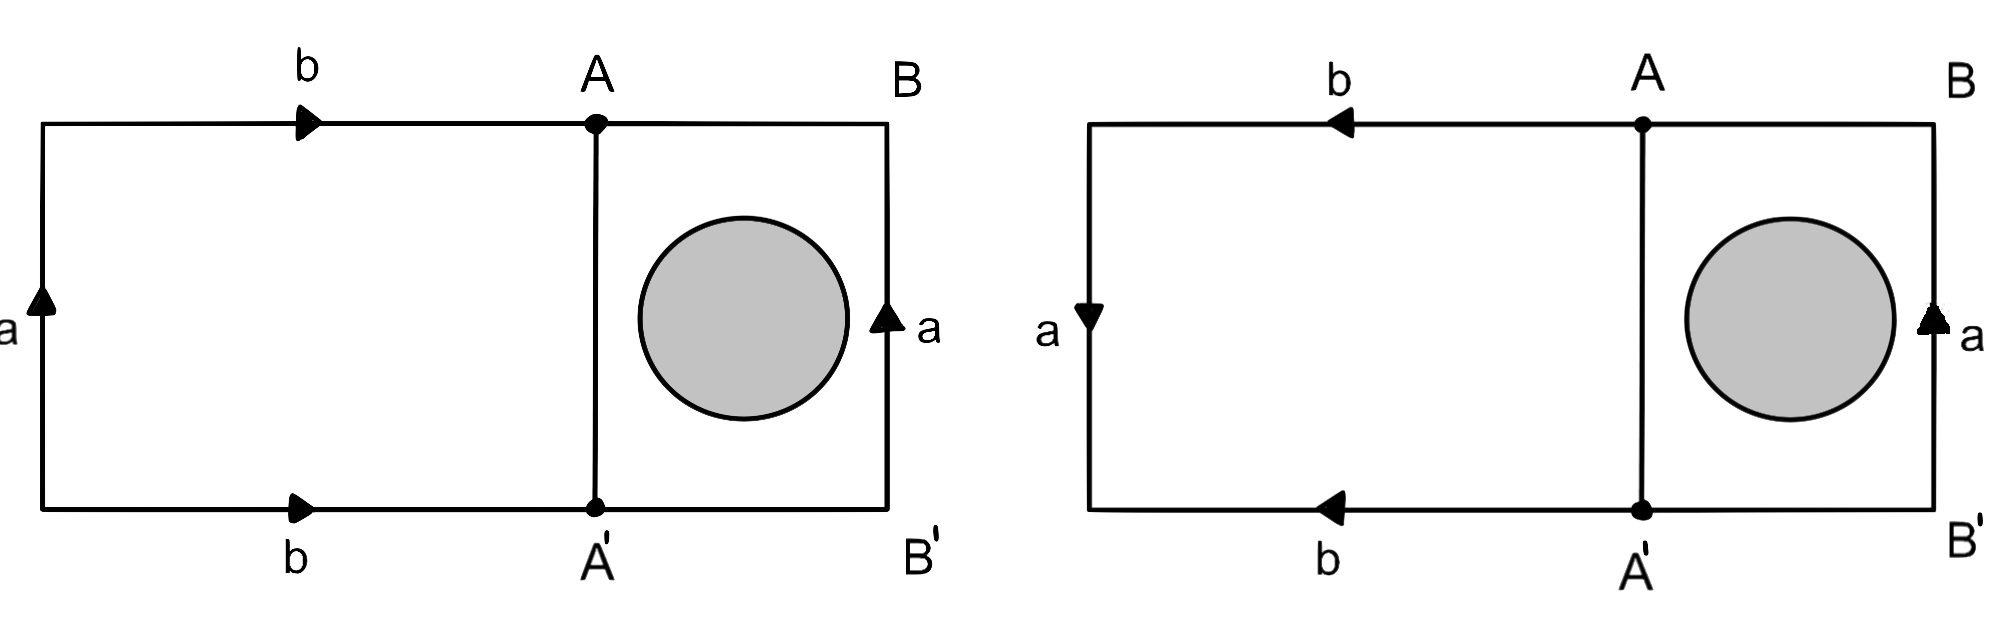
\includegraphics[width=0.5\linewidth]{imagenes/recorte1.png}
	\caption{(a) Toro sin un disco    (b) Botella de Klein sin un disco}
    \label{recorte1}
\end{figure}

Tras el pegar el rectángulo $ABB'A'$, hemos conseguido la suma conexa de $S$ con un cilindro abierto.  Un cilindro es homeomorfo a la esfera con dos agujeros, de modo que, al sumarlo con $S$, la superficie $S$ no se ve alterada salvo por dos discos abiertos que se han eliminado. En el segundo paso, conectaremos los dos agujeros con el resto del toro o botella de Klein. La diferencia entre ambas es la orientación con la que identificaremos los bordes. En el caso del toro los bordes de los discos retirados se identifican manteniendo la orientación, mientras que en el caso de la botella de Klein las orientaciones se invierten. La figura \ref{recorte2} ilustra la suma de $S$ con el toro y la botella de Klein, respectivamente. 

\begin{figure}[h!]
	\centering
	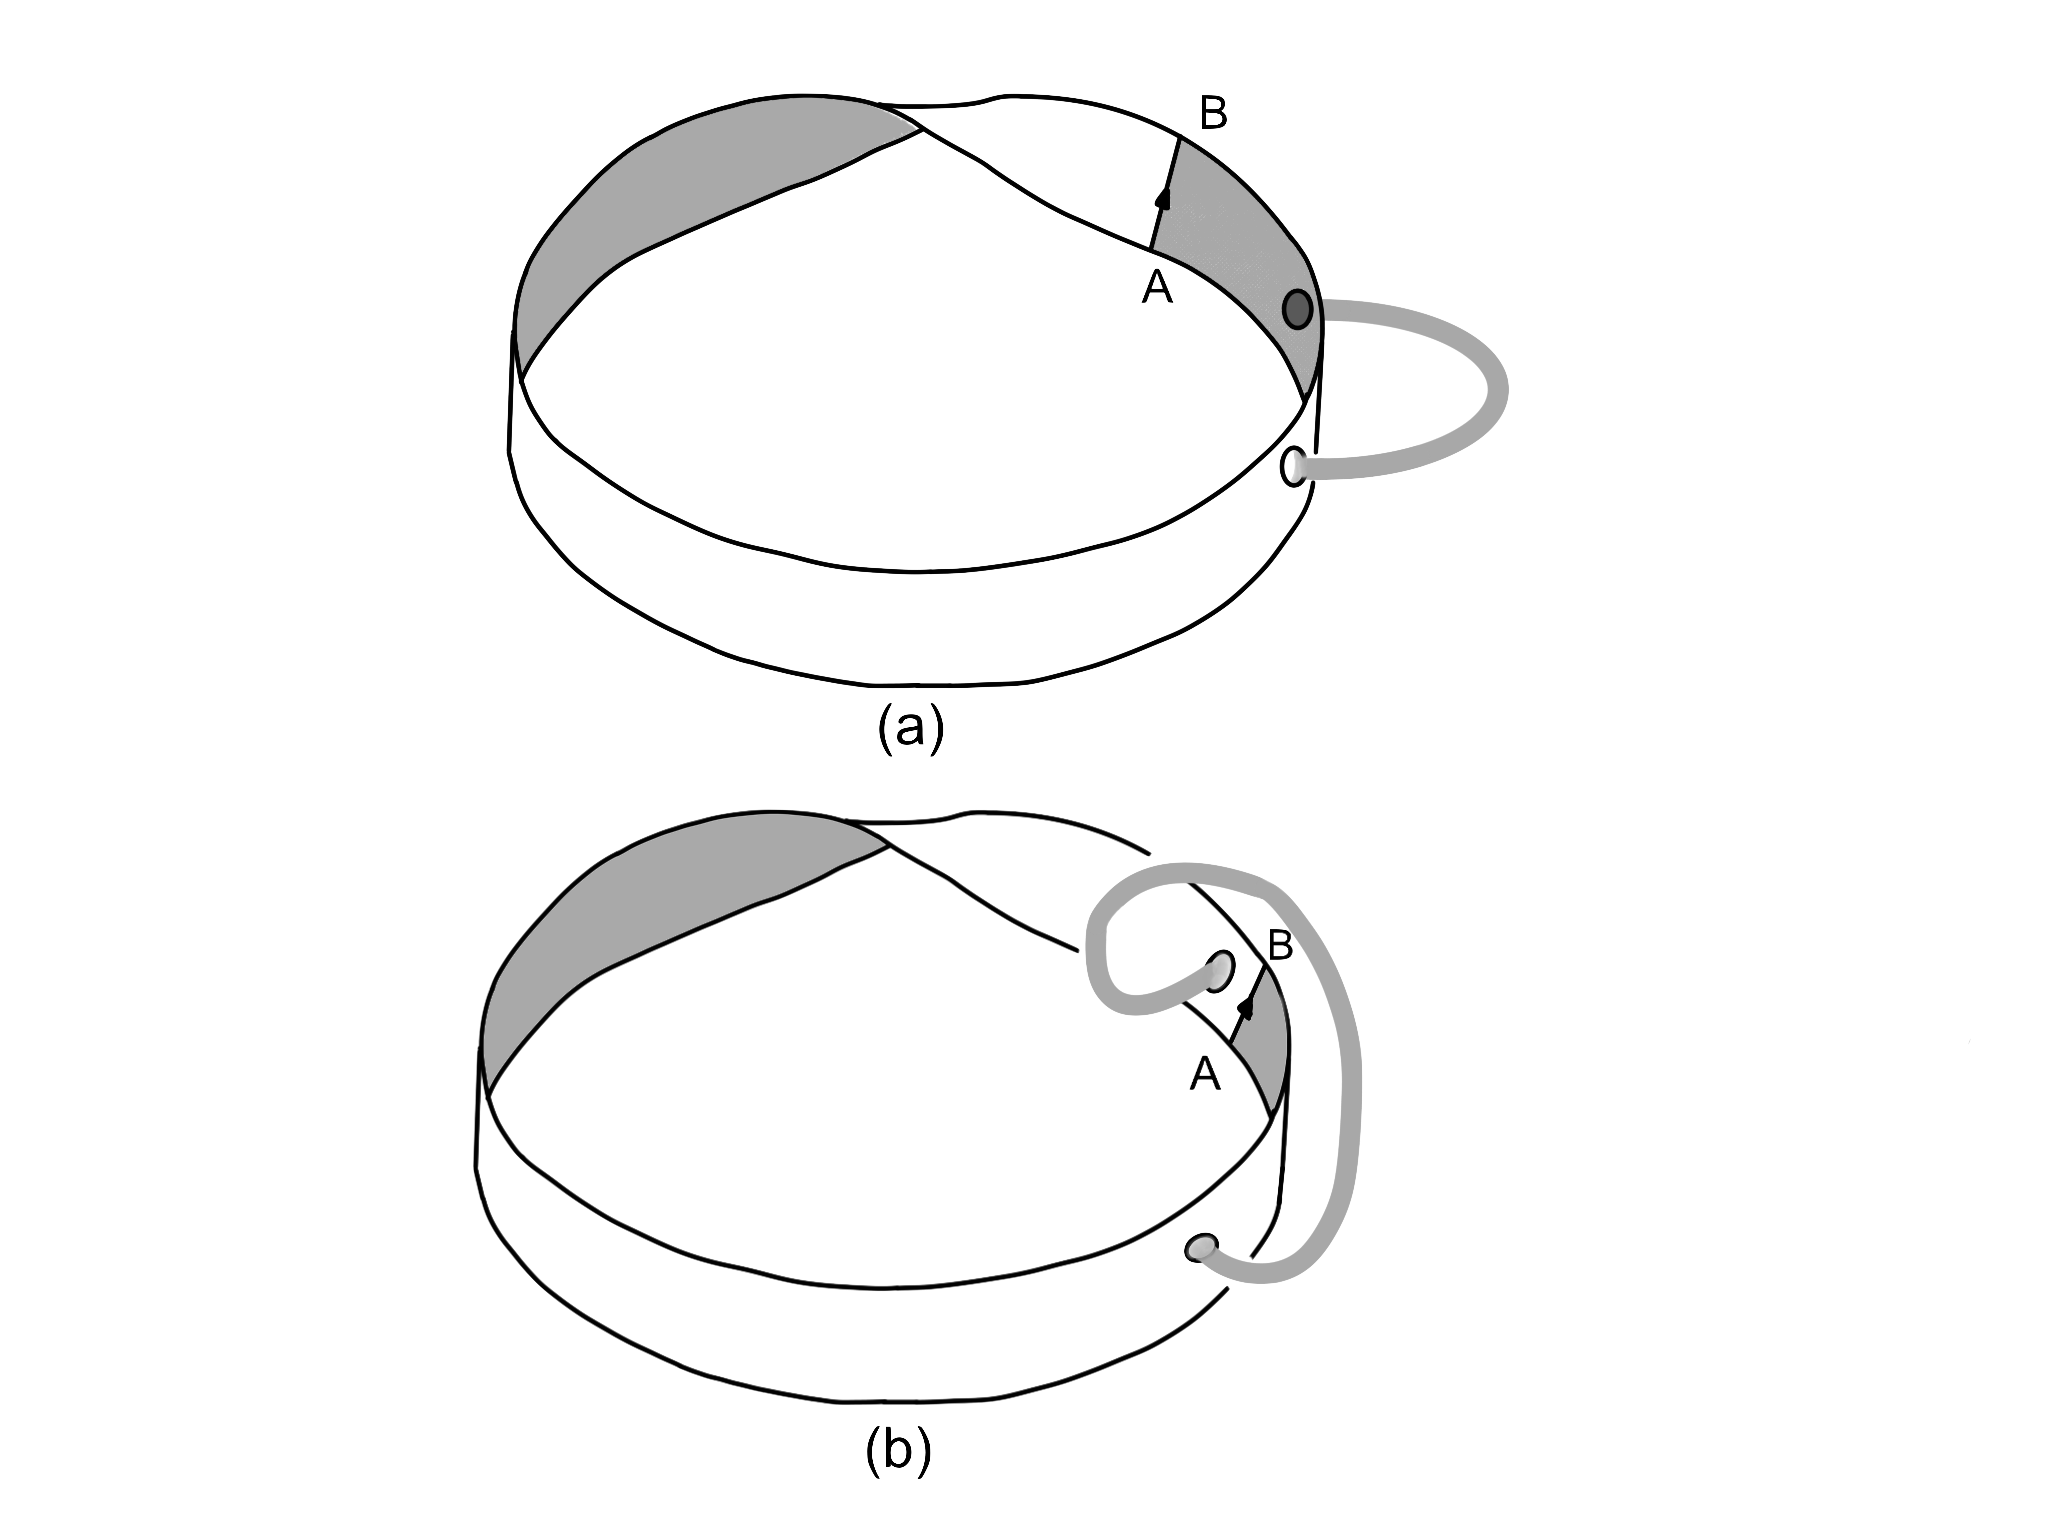
\includegraphics[width=0.5\linewidth]{imagenes/recorte2.png}
	\caption{(a) Suma conexa de toro con banda de M\"obius (b) Suma conexa de botella de Klein con banda de M\"obius}
    \label{recorte2}
\end{figure}

Si recortamos a lo largo de $AB$ en la figura \ref{recorte2}, obtenemos el nuevo rectángulo \ref{recorte3} en la que los lados $AB$ están identificados según señalan las flechas. Esta segunda figura es obtenida con independencia de que se elija la imagen del toro o la de la botella de Klein. Se observa entonces que la suma conexa de un toro con una banda de M\"obius es homeomorfa la suma conexa de una botella de Klein con una banda de M\"obius. Como mencionamos al inicio de la demostración, basta ahora con sumar un disco cerrado al borde de $S$ para obtener una suma de un toro con un plano proyectivo y la suma de una botella de Klein con un plano proyectivo, concluyendo así la demostración.

\begin{figure}[h!]
	\centering
	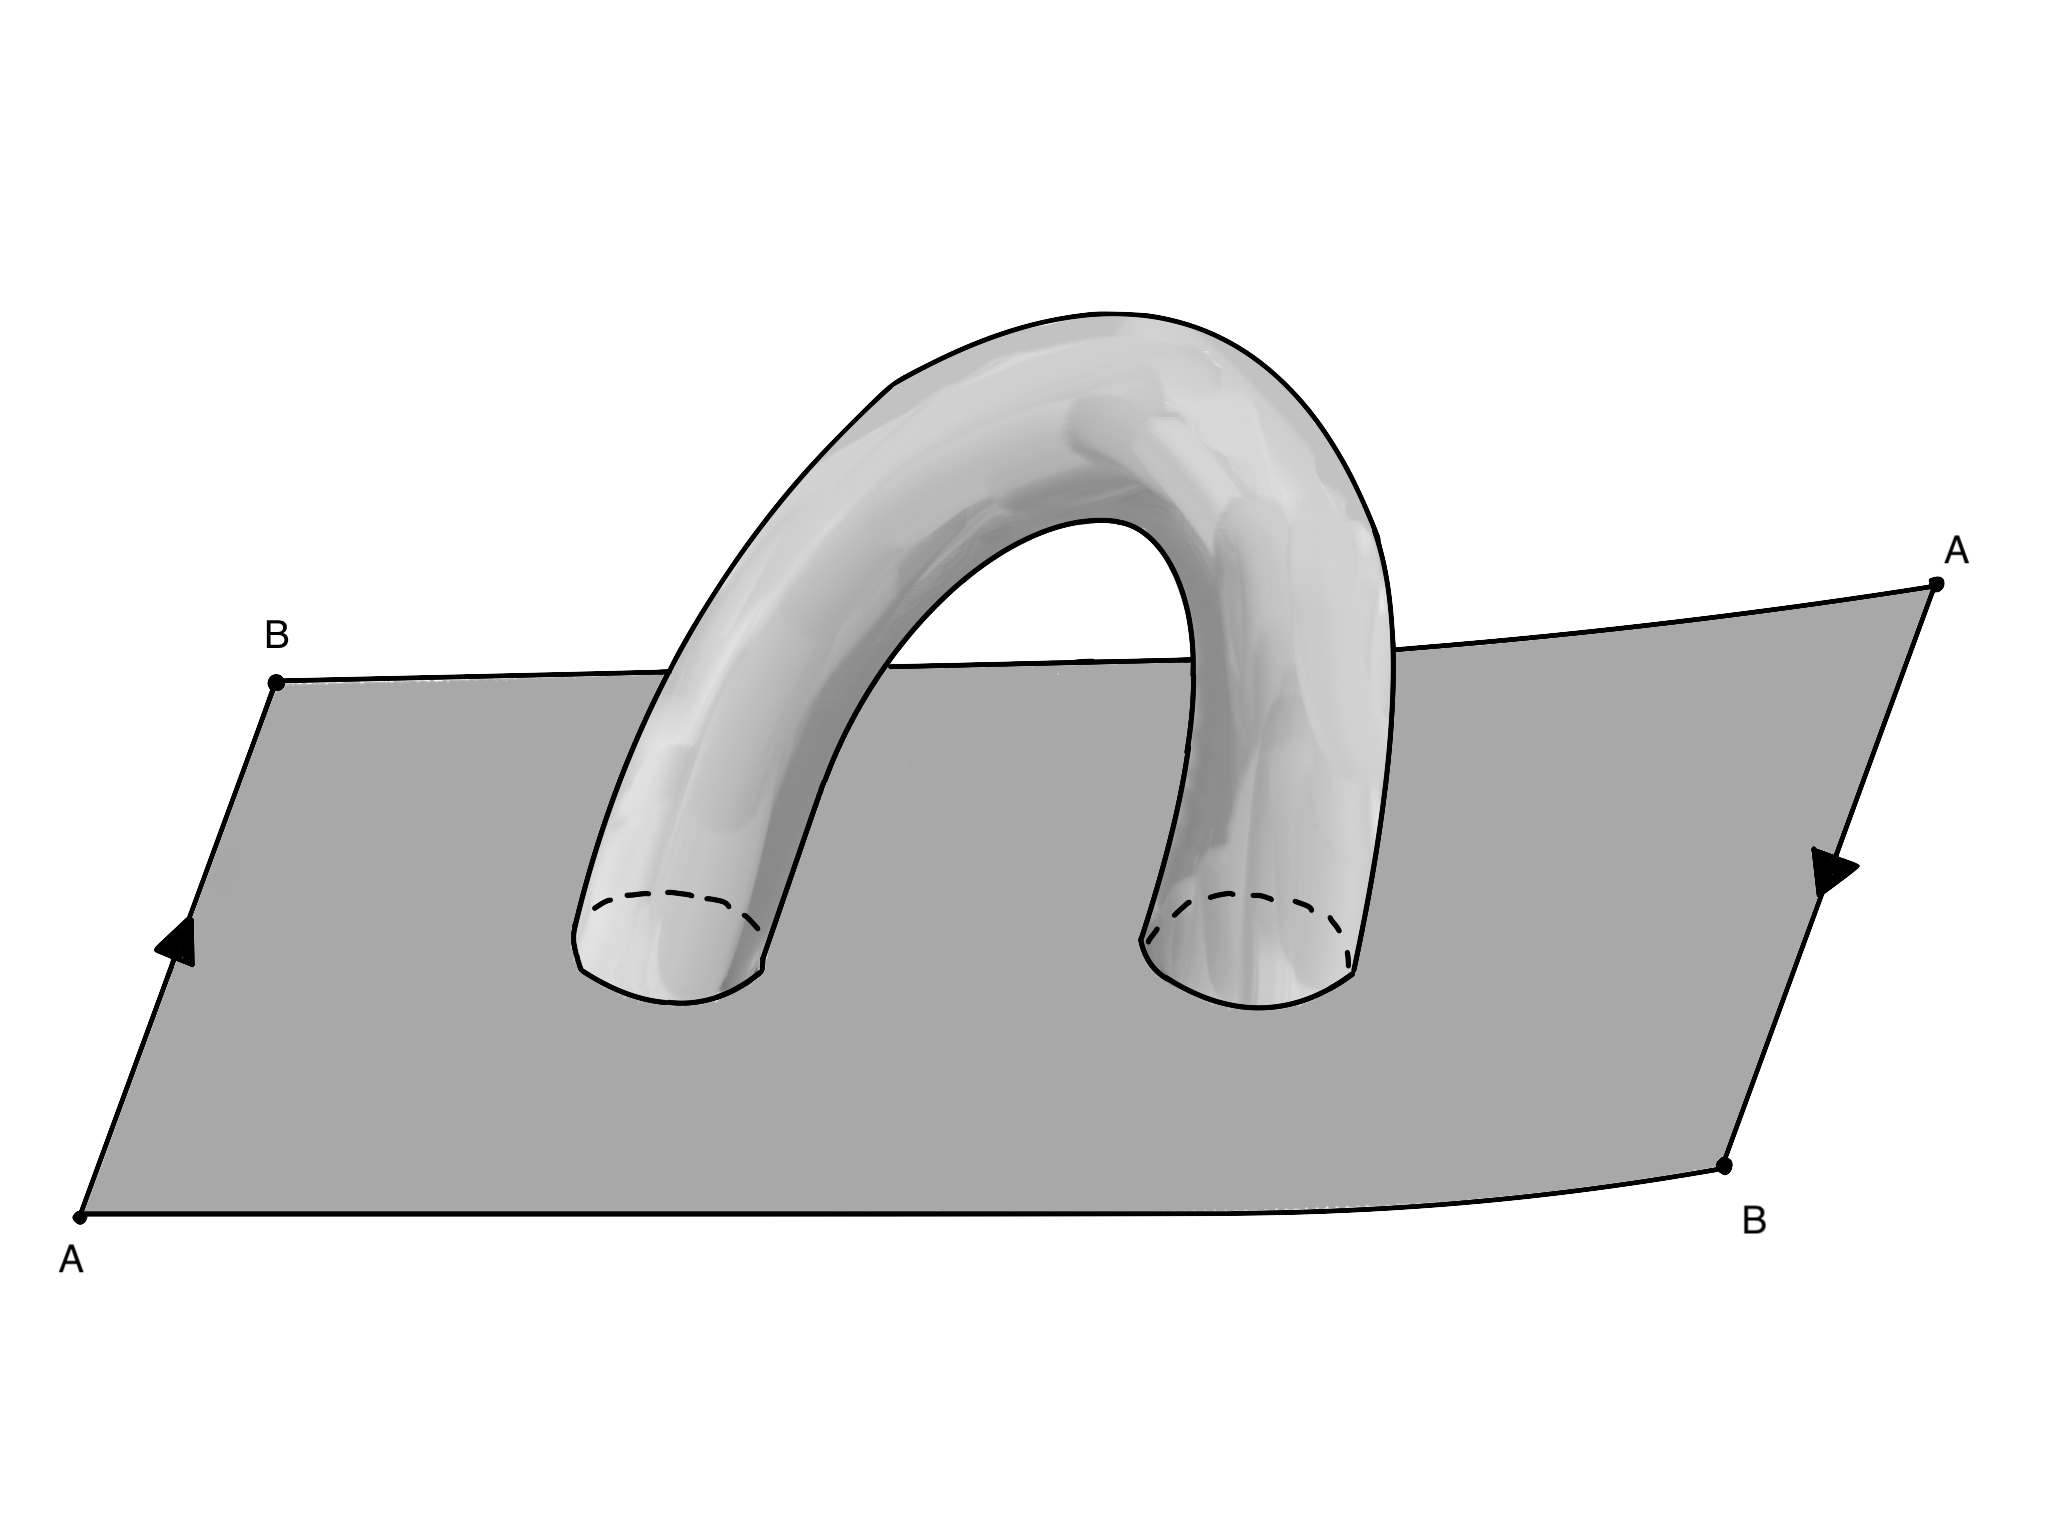
\includegraphics[width=0.3\linewidth]{imagenes/recorte3.png}
	\caption{Resultado de cortar por la línea AB a las figuras de \ref{recorte2}.}
    \label{recorte3}
\end{figure}
\end{proof}

\section{Clasificación de superficies compactas con borde}
\label{anexo:teor1}
\begin{proof}[Demostración del teorema \ref{teor:clasifcompactaconborde}]
Como se comentó en la sección \ref{sec:superfborde}, el ``solo si'' del teorema se sigue de las construcciones de $M_1^*$ y $M_2^*$, demostraremos aquí la parte del ``si''.

Al igual que para la clasificación de superficies compactas demostraremos que la superficies con borde $M_1$ y $M_2$ son homeomorfas a polígonos con ciertos pares de aristas identificados, la llamada \textit{forma normal}. Primero, estudiemos cuáles son estas formas normales.

\begin{figure}[h!]
	\centering
	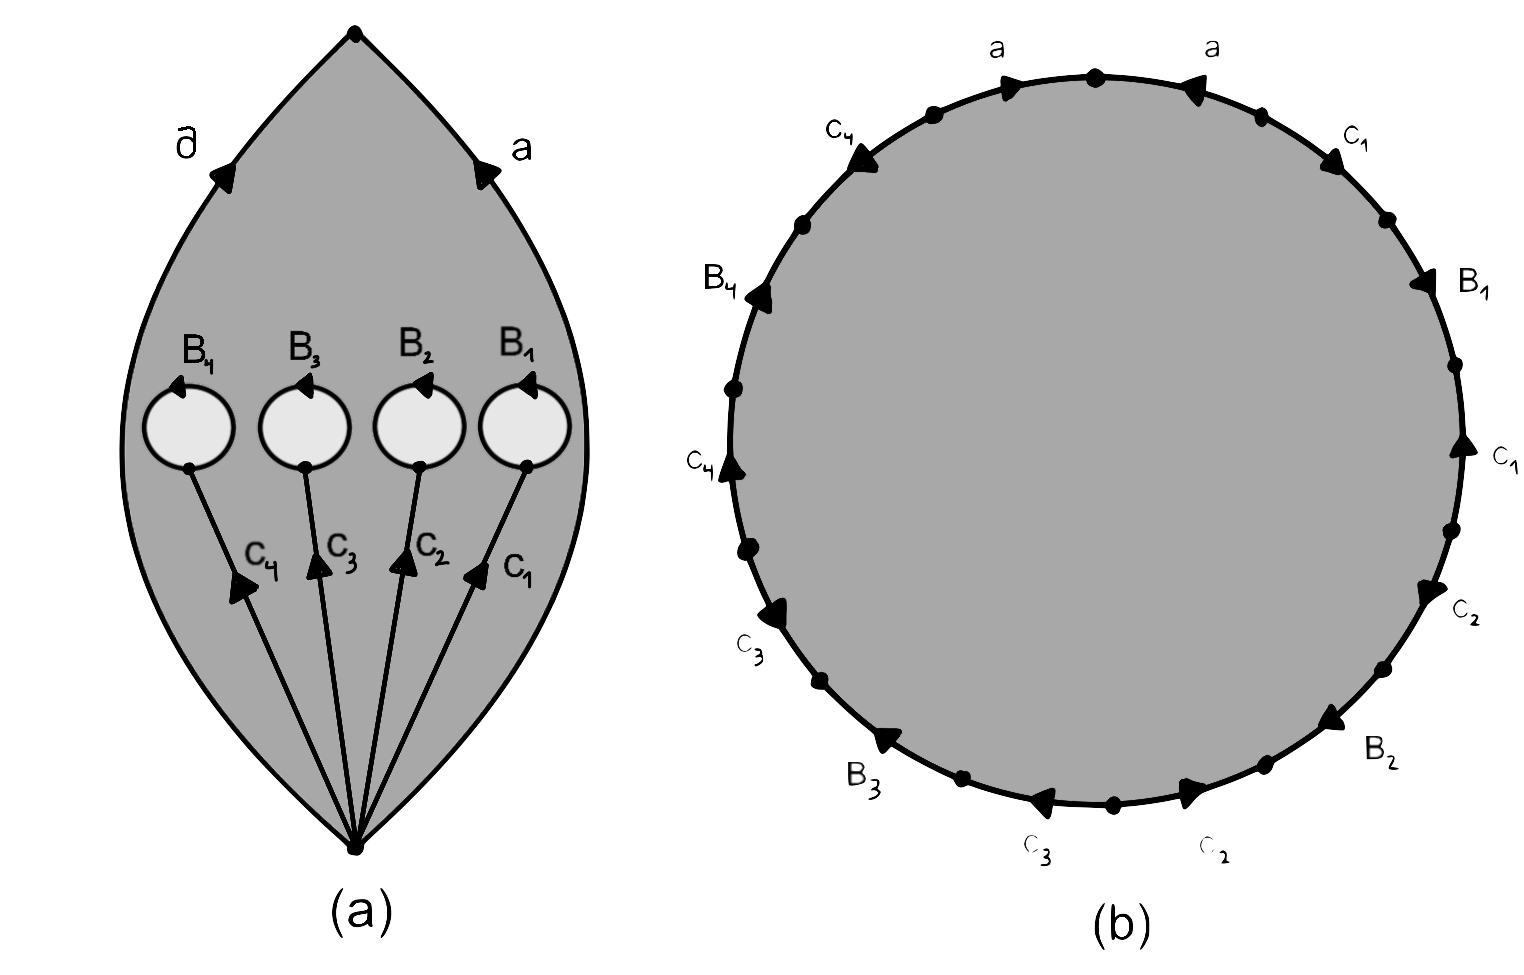
\includegraphics[width=0.5\linewidth]{imagenes/esfera4agujeros.png}
	\caption{Esfera con 4 agujeros.}
    \label{imagen de forma normal de esfera con 4 agujeros}
\end{figure}

\noindent \textbf{Forma normal de una esfera con k agujeros}. La esfera se representa como un polígono con 2 lados cuyas aristas se identifican según la expresión $aa^{-1}$. Hacemos $k$ agujeros, como se indica en la figura \ref{imagen de forma normal de esfera con 4 agujeros} (a) para el caso de $k=4$. Partiendo de un vértice realizamos los cortes $c_1, c_2, \ldots, c_k$ hasta la respectiva componente del borde $B_1, B_2, \ldots, B_k$. Abrimos entonces la figura como se muestra en \ref{imagen de forma normal de esfera con 4 agujeros} (b), teniendo en cuenta que las aristas $c_i$ se desdoblan pero en la nueva expresión son aristas que van identificadas. También es importante destacar que, a diferencia del caso compacto, existen aristas del polígono que no son identificadas con ninguna otra arista, estos lados corresponden justamente con las componentes del borde. Este nuevo polígono obtenido (b) corresponderá con la forma normal buscada. Tenemos entonces que la forma normal de una esfera con $k$ componentes de borde se expresa como:
\[ aa^{-1}c_1B_1c_1^{-1}c_2B_2c_2^{-1}\ldots c_kB_kc_k^{-1} \]

\noindent \textbf{Forma normal de suma conexa de n toros con k agujeros}. La manera de proceder es totalmente análoga al caso anterior: se expresa la forma normal de la suma de n toros para el caso compacto, se retiran $k$ discos abiertos del interior del polígono, se recortan los $k$ segmentos $c_i$ que conecta un único vértice con su respectiva componente de borde y, finalmente, se abre el polígono teniendo en cuenta la identificación de los segmentos $c_i$. De nuevo, el procedimiento se ilustra en la figura \ref{imagen de toro con dos agujeros} para el caso de $n=1$ y $k=2$. En general, el polígono de la forma normal obtenido tendrá $4n+3k$ aristas y se expresará como:
\[ a_1b_1a_1^{-1}b_1^{-1}\ldots a_nb_na_n^{-1}b_n^{-1}c_1B_1c_1^{-1}\ldots c_kB_kc_k^{-1}  \] 

\noindent \textbf{Forma normal de suma conexa de n planos proyectivos con k agujeros}. De nuevo, el procedimiento será análogo. En este caso se obtiene un polígono con $2n+3k$ lados y la expresión será:
\[ a_1a_1\ldots a_na_nc_1B_1c_1^{-1}\ldots c_kB_kc_k^{-1}  \] 

\begin{figure}[h!]
	\centering
	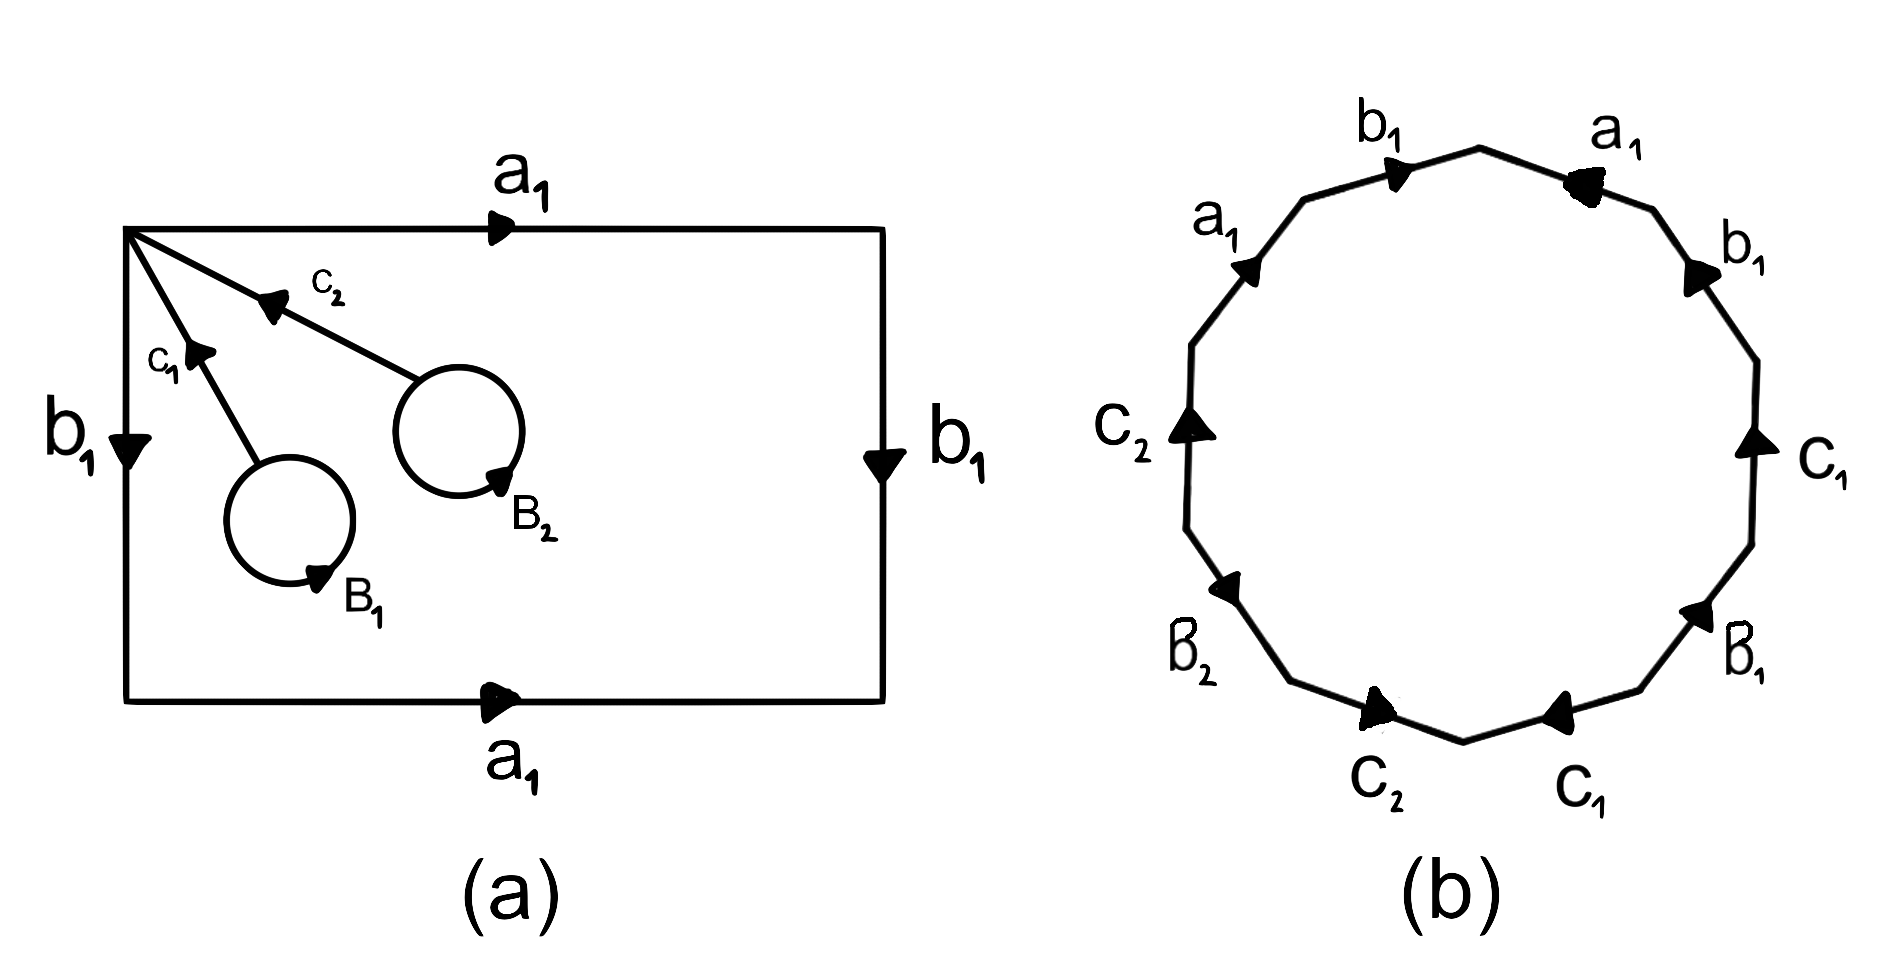
\includegraphics[width=0.5\linewidth]{imagenes/toro2agujeros.png}
	\caption{Toro con dos agujeros.}
    \label{imagen de toro con dos agujeros}
\end{figure}

Para las superficies compactas con borde la noción de triangulación es esencialemente la misma que la dada en el sección \ref{seccion de triangulacion}. Sin embargo, el lema \ref{lema:lema1detriangulacion} es ligeramente diferente para las superficies con borde: una arista podrá bien serlo de exactamente dos triángulos o serlo de un único triángulo, y este segundo caso se dará si y solo si esa arista pertenece al borde de la superficie. Utilizaremos para esta demostración que toda superficie compacta con borde es triangulable, este hecho se sigue del teorema de Tibor Radó y se demuestra en \cite{Ahlfors}.

Consideremos la superficie con borde compacta $M$ y una triangulación dada. Podemos suponer que la triangulación satisface que: cuando una arista tiene dos vértices en el borde, está contenida toda ella en el borde y ningún triángulo tiene más de una arista contenida en el borde (1). En caso de que esta condición no se verifique, se puede conseguir dividiendo el triángulo en otros 6, como muestra la figura \ref{imagen de division baricentrica}, esto es, realizando una \textit{división baricéntrica}. Reutilizando este procedimiento, podemos incluso forzar que la triangulación satisfaga que: si $T_i$ y $T_j$ son triángulos, cada uno con una arista en el borde, entonces  $T_i$ y $T_j$ son o bien disjuntos, o bien comparten un vértice, que a su vez pertenece al borde (2). 

\begin{figure}[h!]
	\centering
	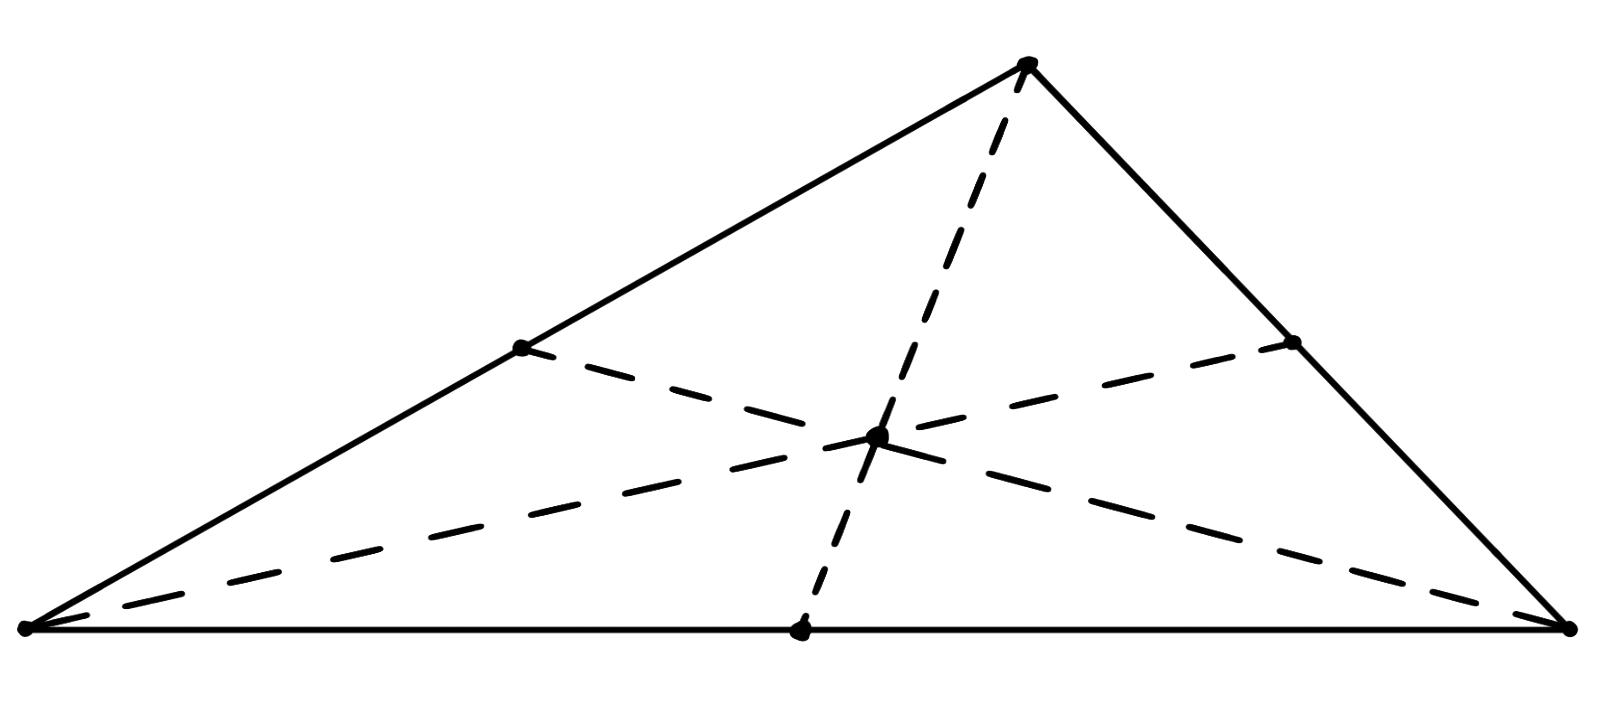
\includegraphics[width=0.3\linewidth]{imagenes/divisionbaricentrica.png}
	\caption{División baricéntrica de un triángulo.}
    \label{imagen de division baricentrica}
\end{figure}

Sean $B_1, \ldots, B_k$ las componentes del borde. Si $T$ es un triángulo que tiene parte común con una de las componentes $B_i$, entonces por (1) hay dos aristas en $T$ que tienen un vértice en común con $B_i$ pero no están contenidas en $B_i$. De la misma manera, si $e$ es una arista que tiene un vértice en $B_i$, sin estar contenida en esta componente de borde, entonces $e$ es arista de dos triángulos que intersecan ambos a $B_i$. Podemos entonces definir una (o más) sucesiones de triángulos y aristas ordenadas
\[T_1, e_1, T_2, e_2, \ldots, T_n, e_n, T_{n+1} = T1\],
donde cada arista $e_j$ lo es de los triángulos $T_{j}$ y $T_{j+1}$, y cada arista tiene un vértice en común con $B_i$ sin estar contenida en $B_i$. Utilizando la definición de triangulación, deducimos que la unión de los triángulos $T_1, T_2, \ldots, T_n$ es homeomorfa a una sección poligonal del plano con un agujero, como la mostrada en la figura \ref{imagen de poligono de borde} para el caso $n=17$. Teniendo en cuenta la conexión de cada componente de borde, se concluye que por cada componente de borde $B_i$ puede existir una única sucesión de las anteriores, y por ende, a cada componente de borde $B_i$ le corresponde una única región poligonal $P_i$.

\begin{figure}[h!]
	\centering
	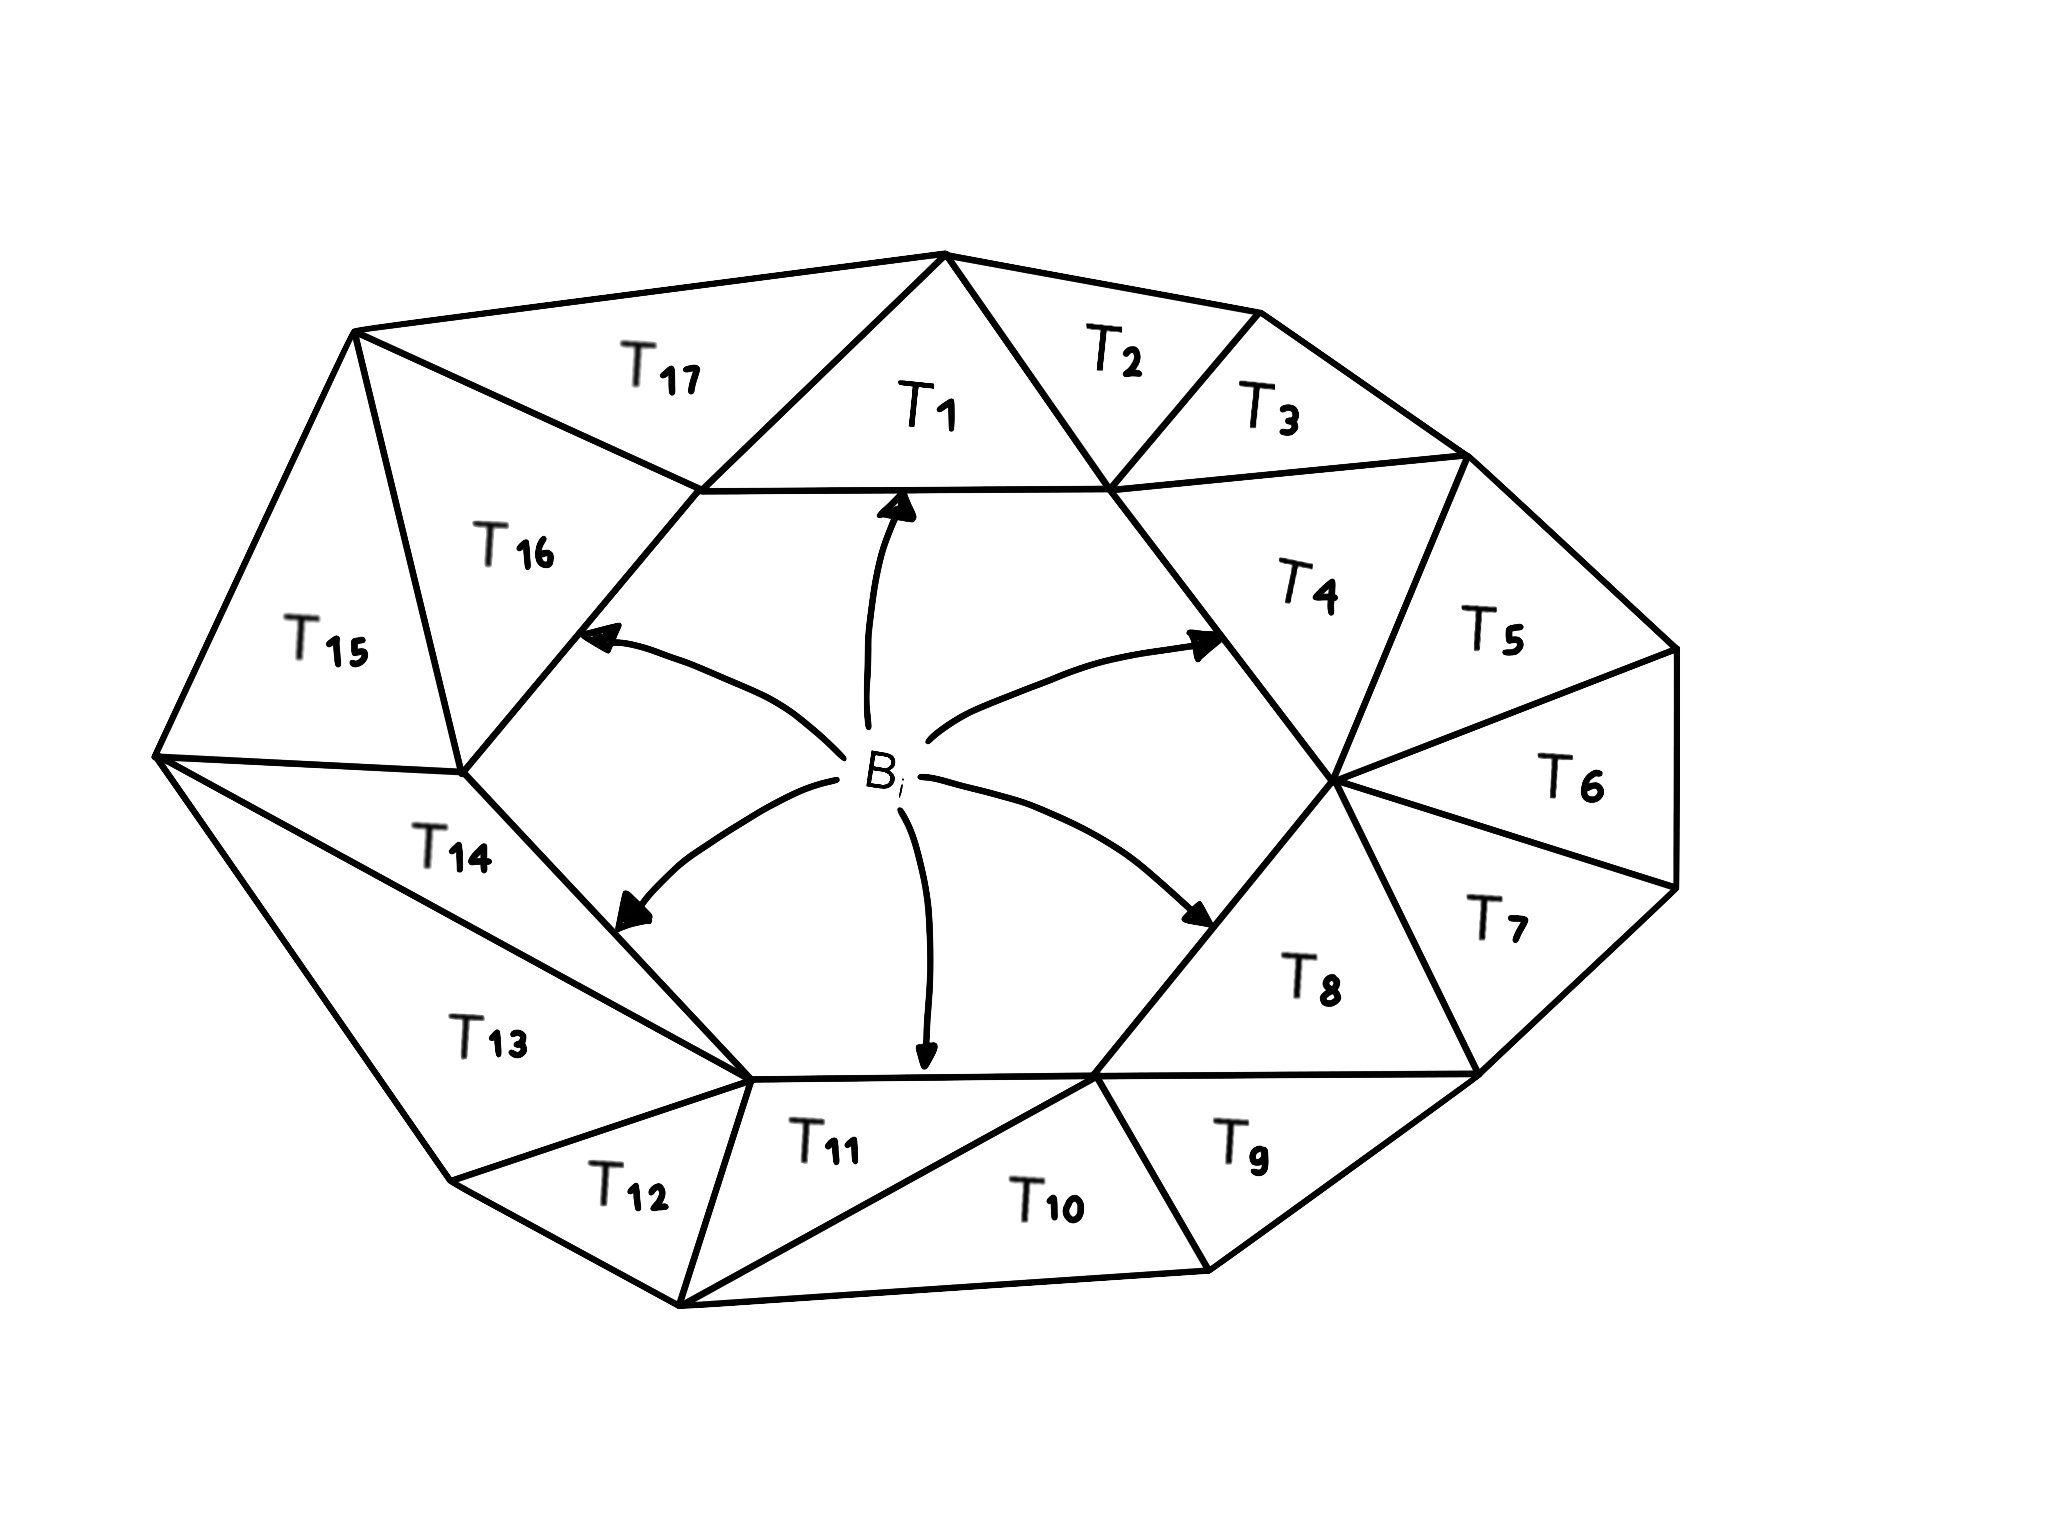
\includegraphics[width=0.5\linewidth]{imagenes/poligonodeborde.png}
	\caption{Polígono $P_i$ obtenido alrededor de una componente de borde $B_i$.}
	\label{imagen de poligono de borde}
\end{figure}

Sean ahora $T_1, \ldots, T_l$ los triángulos de la triangulación dada que no estén contenidos en los polígonos $P_i$, $1 \leq i \leq k$. Usando un razonamiento idéntico al utilizado en el paso 1 de la clasificación compacta (\ref{seccion primer paso}), podemos construir con los $k$  polígonos y los $l$ triángulos, un único polígono con las aristas identificadas a pares y $k$ agujeros en su interior. En la figura \ref{imagen ejemplo de poligono con k=4} se ilustra el caso de posibles polígonos obtenidos con $k=4$.

\begin{figure}[h!]
	\centering
	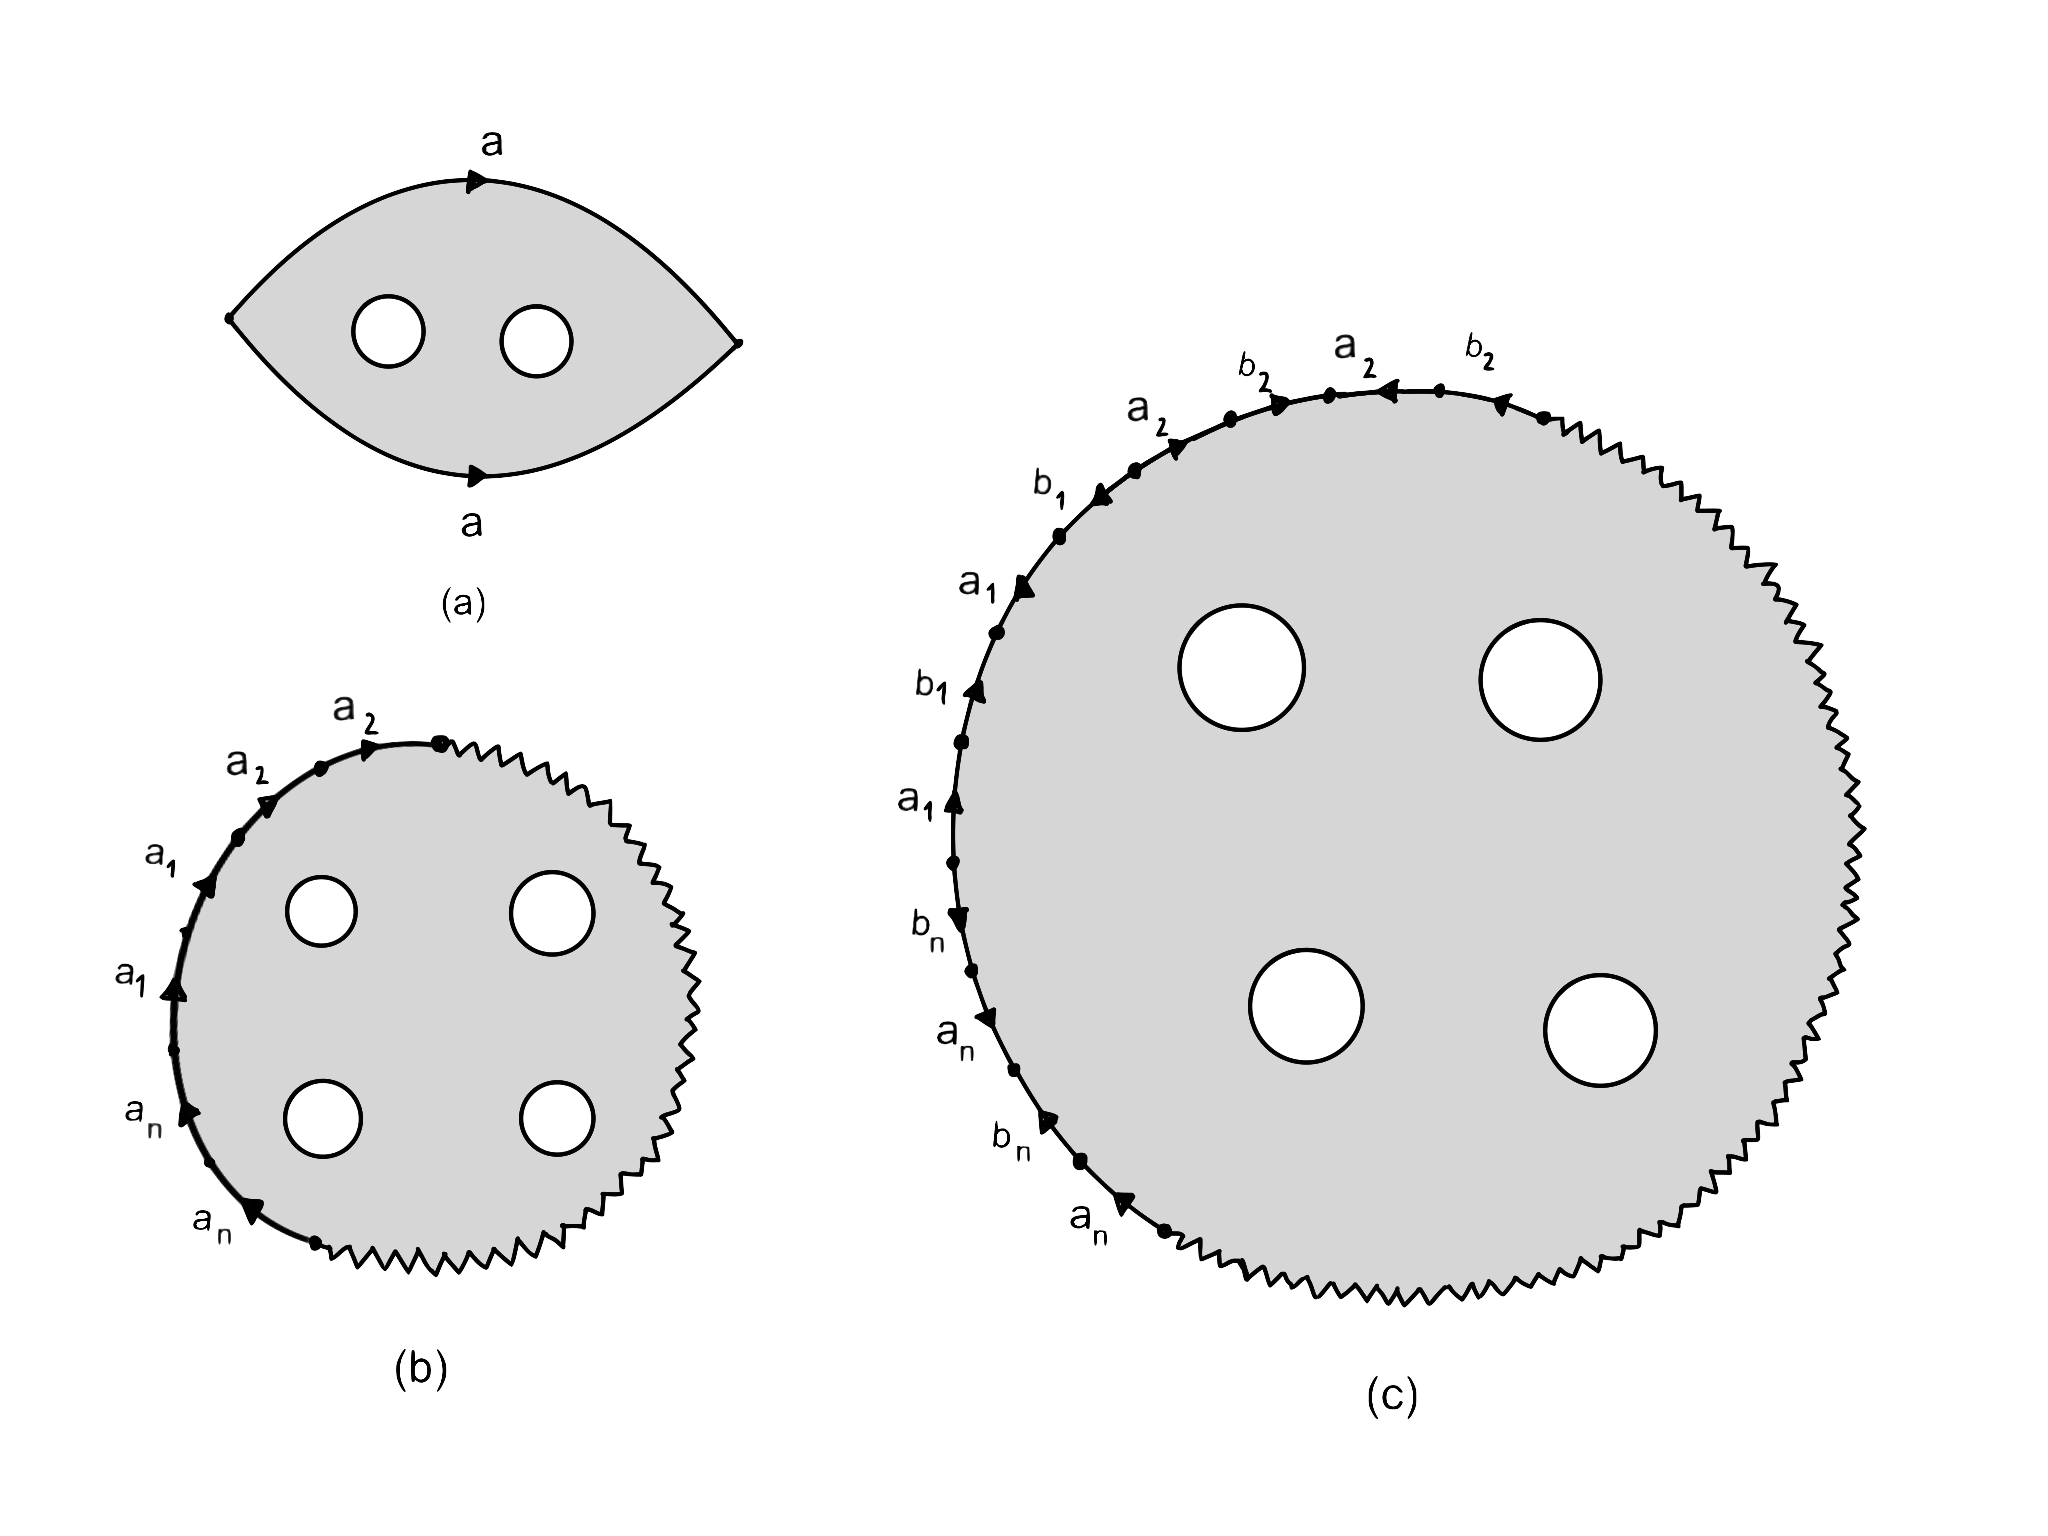
\includegraphics[width=0.5\linewidth]{imagenes/poligonosdesuperficies.png}
	\caption{Polígonos de superficies con borde con $k=4$.}	
    \label{imagen ejemplo de poligono con k=4}
\end{figure}

Una vez se tiene el polígono con los $k$ agujeros y las aristas identificadas a pares, podemos proceder a realizar los mismos pasos que en la clasificación de superficies compactas sin borde (véase el capítulo \ref{chap:clasifcompacta}). Sin embargo, al aplicar los pasos de cortado y pegado se tiene que tener en cuenta que no siempre se podrán hacer cortes en líneas rectas, sino que se tendrán que evitar los agujeros. Al ser $k$ un número finito, resulta evidente que los pasos se pueden realizar. Además, está claro que el número de agujeros $k$ no se ve alterado tras cada paso. Finalmente, obtendremos como resultado un polígono correspondiente a una de las expresiones canónicas ya estudiadas en la sección \ref{subsec:expresionescanonicassumasconexas}, pero con $k$ agujeros en su interior. La figura \ref{imagen ejemplo de poligono con k=4} muestra los tres posibles casos para $k=4$: (a) Una esfera con cuatro agujeros, (b) la suma conexa de $n$ planos proyectivos con cuatro agujeros, y (c) la suma conexa de $n$ toros con cuatro agujeros.\\
Realizando los correspondientes cortes $c_1, \ldots, c_k$ a cada una de las componentes de borde y `abriendo' el polígono, queda claro que obtenemos una de las expresiones canónicas estudiadas al inicio de la demostración. 

Nótese que la construcción propuesta determina topológicamente a una superficie con borde compacta $M$, utilizando únicamente el tipo topológico de $M^*$ y el número de componentes de borde, finalizando así la demostración del teorema.

\end{proof}







\begin{thebibliography}{10}
%% TODO: VER COMO SE TIENEN QUE PONER LAS CITAS
\bibitem{massey} 
    \textsc{William S. Massey}, 
    Introducción a la topología algebraica. \textit{Reverté}, 2006.
    
\bibitem{ian}
    \textsc{I. Richards},
    On the classification of noncompact surfaces. \textit{Trans. Amer. Math. Soc.} 106 (1963), 259–269

\bibitem{Ahlfors}
    \textsc{Ahlfors L. V.} y \textsc{Sario},
    Riemann Surfaces. \textit{Princeton University Press}, 1960.

\bibitem{cerradoscantor}
   \textsc{M. Reichbach},
    The power of topological types of some classes of 0-dimensional sets. \textit{Proc. Amer. Math. Soc.} 13 (1962), 17–23.   
    

\bibitem{nosegundonomuerable}
   \textsc{D. Gauld}, Non-metrisable manifolds. \textit{Springer, Singapore,} 2014. xvi+203 pp. 

    
\end{thebibliography}
\cleardoublepage
\end{document}
